% Options for packages loaded elsewhere
\PassOptionsToPackage{unicode}{hyperref}
\PassOptionsToPackage{hyphens}{url}
\PassOptionsToPackage{dvipsnames,svgnames,x11names}{xcolor}
%
\documentclass[
  a4paper,
  DIV=11]{scrreprt}

\usepackage{amsmath,amssymb}
\usepackage{lmodern}
\usepackage{iftex}
\ifPDFTeX
  \usepackage[T1]{fontenc}
  \usepackage[utf8]{inputenc}
  \usepackage{textcomp} % provide euro and other symbols
\else % if luatex or xetex
  \usepackage{unicode-math}
  \defaultfontfeatures{Scale=MatchLowercase}
  \defaultfontfeatures[\rmfamily]{Ligatures=TeX,Scale=1}
\fi
% Use upquote if available, for straight quotes in verbatim environments
\IfFileExists{upquote.sty}{\usepackage{upquote}}{}
\IfFileExists{microtype.sty}{% use microtype if available
  \usepackage[]{microtype}
  \UseMicrotypeSet[protrusion]{basicmath} % disable protrusion for tt fonts
}{}
\makeatletter
\@ifundefined{KOMAClassName}{% if non-KOMA class
  \IfFileExists{parskip.sty}{%
    \usepackage{parskip}
  }{% else
    \setlength{\parindent}{0pt}
    \setlength{\parskip}{6pt plus 2pt minus 1pt}}
}{% if KOMA class
  \KOMAoptions{parskip=half}}
\makeatother
\usepackage{xcolor}
\setlength{\emergencystretch}{3em} % prevent overfull lines
\setcounter{secnumdepth}{5}
% Make \paragraph and \subparagraph free-standing
\ifx\paragraph\undefined\else
  \let\oldparagraph\paragraph
  \renewcommand{\paragraph}[1]{\oldparagraph{#1}\mbox{}}
\fi
\ifx\subparagraph\undefined\else
  \let\oldsubparagraph\subparagraph
  \renewcommand{\subparagraph}[1]{\oldsubparagraph{#1}\mbox{}}
\fi

\usepackage{color}
\usepackage{fancyvrb}
\newcommand{\VerbBar}{|}
\newcommand{\VERB}{\Verb[commandchars=\\\{\}]}
\DefineVerbatimEnvironment{Highlighting}{Verbatim}{commandchars=\\\{\}}
% Add ',fontsize=\small' for more characters per line
\usepackage{framed}
\definecolor{shadecolor}{RGB}{241,243,245}
\newenvironment{Shaded}{\begin{snugshade}}{\end{snugshade}}
\newcommand{\AlertTok}[1]{\textcolor[rgb]{0.68,0.00,0.00}{#1}}
\newcommand{\AnnotationTok}[1]{\textcolor[rgb]{0.37,0.37,0.37}{#1}}
\newcommand{\AttributeTok}[1]{\textcolor[rgb]{0.40,0.45,0.13}{#1}}
\newcommand{\BaseNTok}[1]{\textcolor[rgb]{0.68,0.00,0.00}{#1}}
\newcommand{\BuiltInTok}[1]{\textcolor[rgb]{0.00,0.23,0.31}{#1}}
\newcommand{\CharTok}[1]{\textcolor[rgb]{0.13,0.47,0.30}{#1}}
\newcommand{\CommentTok}[1]{\textcolor[rgb]{0.37,0.37,0.37}{#1}}
\newcommand{\CommentVarTok}[1]{\textcolor[rgb]{0.37,0.37,0.37}{\textit{#1}}}
\newcommand{\ConstantTok}[1]{\textcolor[rgb]{0.56,0.35,0.01}{#1}}
\newcommand{\ControlFlowTok}[1]{\textcolor[rgb]{0.00,0.23,0.31}{#1}}
\newcommand{\DataTypeTok}[1]{\textcolor[rgb]{0.68,0.00,0.00}{#1}}
\newcommand{\DecValTok}[1]{\textcolor[rgb]{0.68,0.00,0.00}{#1}}
\newcommand{\DocumentationTok}[1]{\textcolor[rgb]{0.37,0.37,0.37}{\textit{#1}}}
\newcommand{\ErrorTok}[1]{\textcolor[rgb]{0.68,0.00,0.00}{#1}}
\newcommand{\ExtensionTok}[1]{\textcolor[rgb]{0.00,0.23,0.31}{#1}}
\newcommand{\FloatTok}[1]{\textcolor[rgb]{0.68,0.00,0.00}{#1}}
\newcommand{\FunctionTok}[1]{\textcolor[rgb]{0.28,0.35,0.67}{#1}}
\newcommand{\ImportTok}[1]{\textcolor[rgb]{0.00,0.46,0.62}{#1}}
\newcommand{\InformationTok}[1]{\textcolor[rgb]{0.37,0.37,0.37}{#1}}
\newcommand{\KeywordTok}[1]{\textcolor[rgb]{0.00,0.23,0.31}{#1}}
\newcommand{\NormalTok}[1]{\textcolor[rgb]{0.00,0.23,0.31}{#1}}
\newcommand{\OperatorTok}[1]{\textcolor[rgb]{0.37,0.37,0.37}{#1}}
\newcommand{\OtherTok}[1]{\textcolor[rgb]{0.00,0.23,0.31}{#1}}
\newcommand{\PreprocessorTok}[1]{\textcolor[rgb]{0.68,0.00,0.00}{#1}}
\newcommand{\RegionMarkerTok}[1]{\textcolor[rgb]{0.00,0.23,0.31}{#1}}
\newcommand{\SpecialCharTok}[1]{\textcolor[rgb]{0.37,0.37,0.37}{#1}}
\newcommand{\SpecialStringTok}[1]{\textcolor[rgb]{0.13,0.47,0.30}{#1}}
\newcommand{\StringTok}[1]{\textcolor[rgb]{0.13,0.47,0.30}{#1}}
\newcommand{\VariableTok}[1]{\textcolor[rgb]{0.07,0.07,0.07}{#1}}
\newcommand{\VerbatimStringTok}[1]{\textcolor[rgb]{0.13,0.47,0.30}{#1}}
\newcommand{\WarningTok}[1]{\textcolor[rgb]{0.37,0.37,0.37}{\textit{#1}}}

\providecommand{\tightlist}{%
  \setlength{\itemsep}{0pt}\setlength{\parskip}{0pt}}\usepackage{longtable,booktabs,array}
\usepackage{calc} % for calculating minipage widths
% Correct order of tables after \paragraph or \subparagraph
\usepackage{etoolbox}
\makeatletter
\patchcmd\longtable{\par}{\if@noskipsec\mbox{}\fi\par}{}{}
\makeatother
% Allow footnotes in longtable head/foot
\IfFileExists{footnotehyper.sty}{\usepackage{footnotehyper}}{\usepackage{footnote}}
\makesavenoteenv{longtable}
\usepackage{graphicx}
\makeatletter
\def\maxwidth{\ifdim\Gin@nat@width>\linewidth\linewidth\else\Gin@nat@width\fi}
\def\maxheight{\ifdim\Gin@nat@height>\textheight\textheight\else\Gin@nat@height\fi}
\makeatother
% Scale images if necessary, so that they will not overflow the page
% margins by default, and it is still possible to overwrite the defaults
% using explicit options in \includegraphics[width, height, ...]{}
\setkeys{Gin}{width=\maxwidth,height=\maxheight,keepaspectratio}
% Set default figure placement to htbp
\makeatletter
\def\fps@figure{htbp}
\makeatother
\newlength{\cslhangindent}
\setlength{\cslhangindent}{1.5em}
\newlength{\csllabelwidth}
\setlength{\csllabelwidth}{3em}
\newlength{\cslentryspacingunit} % times entry-spacing
\setlength{\cslentryspacingunit}{\parskip}
\newenvironment{CSLReferences}[2] % #1 hanging-ident, #2 entry spacing
 {% don't indent paragraphs
  \setlength{\parindent}{0pt}
  % turn on hanging indent if param 1 is 1
  \ifodd #1
  \let\oldpar\par
  \def\par{\hangindent=\cslhangindent\oldpar}
  \fi
  % set entry spacing
  \setlength{\parskip}{#2\cslentryspacingunit}
 }%
 {}
\usepackage{calc}
\newcommand{\CSLBlock}[1]{#1\hfill\break}
\newcommand{\CSLLeftMargin}[1]{\parbox[t]{\csllabelwidth}{#1}}
\newcommand{\CSLRightInline}[1]{\parbox[t]{\linewidth - \csllabelwidth}{#1}\break}
\newcommand{\CSLIndent}[1]{\hspace{\cslhangindent}#1}

\KOMAoption{captions}{tableheading}
\makeatletter
\@ifpackageloaded{tcolorbox}{}{\usepackage[many]{tcolorbox}}
\@ifpackageloaded{fontawesome5}{}{\usepackage{fontawesome5}}
\definecolor{quarto-callout-color}{HTML}{909090}
\definecolor{quarto-callout-note-color}{HTML}{0758E5}
\definecolor{quarto-callout-important-color}{HTML}{CC1914}
\definecolor{quarto-callout-warning-color}{HTML}{EB9113}
\definecolor{quarto-callout-tip-color}{HTML}{00A047}
\definecolor{quarto-callout-caution-color}{HTML}{FC5300}
\definecolor{quarto-callout-color-frame}{HTML}{acacac}
\definecolor{quarto-callout-note-color-frame}{HTML}{4582ec}
\definecolor{quarto-callout-important-color-frame}{HTML}{d9534f}
\definecolor{quarto-callout-warning-color-frame}{HTML}{f0ad4e}
\definecolor{quarto-callout-tip-color-frame}{HTML}{02b875}
\definecolor{quarto-callout-caution-color-frame}{HTML}{fd7e14}
\makeatother
\makeatletter
\makeatother
\makeatletter
\@ifpackageloaded{bookmark}{}{\usepackage{bookmark}}
\makeatother
\makeatletter
\@ifpackageloaded{caption}{}{\usepackage{caption}}
\AtBeginDocument{%
\ifdefined\contentsname
  \renewcommand*\contentsname{Inhaltsverzeichnis}
\else
  \newcommand\contentsname{Inhaltsverzeichnis}
\fi
\ifdefined\listfigurename
  \renewcommand*\listfigurename{Abbildungsverzeichnis}
\else
  \newcommand\listfigurename{Abbildungsverzeichnis}
\fi
\ifdefined\listtablename
  \renewcommand*\listtablename{Tabellenverzeichnis}
\else
  \newcommand\listtablename{Tabellenverzeichnis}
\fi
\ifdefined\figurename
  \renewcommand*\figurename{Abbildung}
\else
  \newcommand\figurename{Abbildung}
\fi
\ifdefined\tablename
  \renewcommand*\tablename{Tabelle}
\else
  \newcommand\tablename{Tabelle}
\fi
}
\@ifpackageloaded{float}{}{\usepackage{float}}
\floatstyle{ruled}
\@ifundefined{c@chapter}{\newfloat{codelisting}{h}{lop}}{\newfloat{codelisting}{h}{lop}[chapter]}
\floatname{codelisting}{Listing}
\newcommand*\listoflistings{\listof{codelisting}{Listingverzeichnis}}
\makeatother
\makeatletter
\@ifpackageloaded{caption}{}{\usepackage{caption}}
\@ifpackageloaded{subcaption}{}{\usepackage{subcaption}}
\makeatother
\makeatletter
\@ifpackageloaded{tcolorbox}{}{\usepackage[many]{tcolorbox}}
\makeatother
\makeatletter
\@ifundefined{shadecolor}{\definecolor{shadecolor}{rgb}{.97, .97, .97}}
\makeatother
\makeatletter
\makeatother
\ifLuaTeX
\usepackage[bidi=basic]{babel}
\else
\usepackage[bidi=default]{babel}
\fi
\babelprovide[main,import]{ngerman}
% get rid of language-specific shorthands (see #6817):
\let\LanguageShortHands\languageshorthands
\def\languageshorthands#1{}
\ifLuaTeX
  \usepackage{selnolig}  % disable illegal ligatures
\fi
\IfFileExists{bookmark.sty}{\usepackage{bookmark}}{\usepackage{hyperref}}
\IfFileExists{xurl.sty}{\usepackage{xurl}}{} % add URL line breaks if available
\urlstyle{same} % disable monospaced font for URLs
\hypersetup{
  pdftitle={Physik der Hochatmosphäre},
  pdfauthor={Dr.~Ralph-Uwe Börner},
  pdflang={de},
  colorlinks=true,
  linkcolor={blue},
  filecolor={Maroon},
  citecolor={Blue},
  urlcolor={Blue},
  pdfcreator={LaTeX via pandoc}}

\title{Physik der Hochatmosphäre}
\usepackage{etoolbox}
\makeatletter
\providecommand{\subtitle}[1]{% add subtitle to \maketitle
  \apptocmd{\@title}{\par {\large #1 \par}}{}{}
}
\makeatother
\subtitle{Modul: Ausgewählte Kapitel der Allgemeinen Geophysik}
\author{Dr.~Ralph-Uwe Börner}
\date{21.11.22}

\begin{document}
\maketitle
\ifdefined\Shaded\renewenvironment{Shaded}{\begin{tcolorbox}[interior hidden, frame hidden, boxrule=0pt, breakable, borderline west={3pt}{0pt}{shadecolor}, sharp corners, enhanced]}{\end{tcolorbox}}\fi

\renewcommand*\contentsname{Inhaltsverzeichnis}
{
\hypersetup{linkcolor=}
\setcounter{tocdepth}{2}
\tableofcontents
}
\bookmarksetup{startatroot}

\hypertarget{vorbemerkung}{%
\chapter{Vorbemerkung}\label{vorbemerkung}}

Das Skript zur Vorlesung ``Physik der Hochatmosphäre'' entsteht
semesterbegleitend und erhebt nicht den Anspruch auf
\href{https://imgflip.com/i/6zt09v}{Vollständigkeit} und Korrektheit.

Es wird mit \href{http://quarto.org}{Quarto}, einem Open-Source-System
zum wissenschaftlichen und technischen Publizieren, entwickelt.

Alle Änderungen sind in \href{https://github.com/ruboerner/PDA}{GitHub}
nachvollziehbar. Ein PDF-Dokument mit aktuellem Inhalt kann dort
heruntergeladen werden.

\part{Einführung}

\hypertarget{einfuxfchrung-1}{%
\chapter{Einführung}\label{einfuxfchrung-1}}

Diese Einführung beruht zum großen Teil auf dem Buch von Kertz (1971).
Dort werden grundlegende Zusammenhänge zur Physik der Hochatmosphäre
physikalisch und mathematisch gut aufbereitet und erläutet. Zum
Selbststudium ist dieses Buch sehr zu empfehlen.

\begin{figure}

{\centering 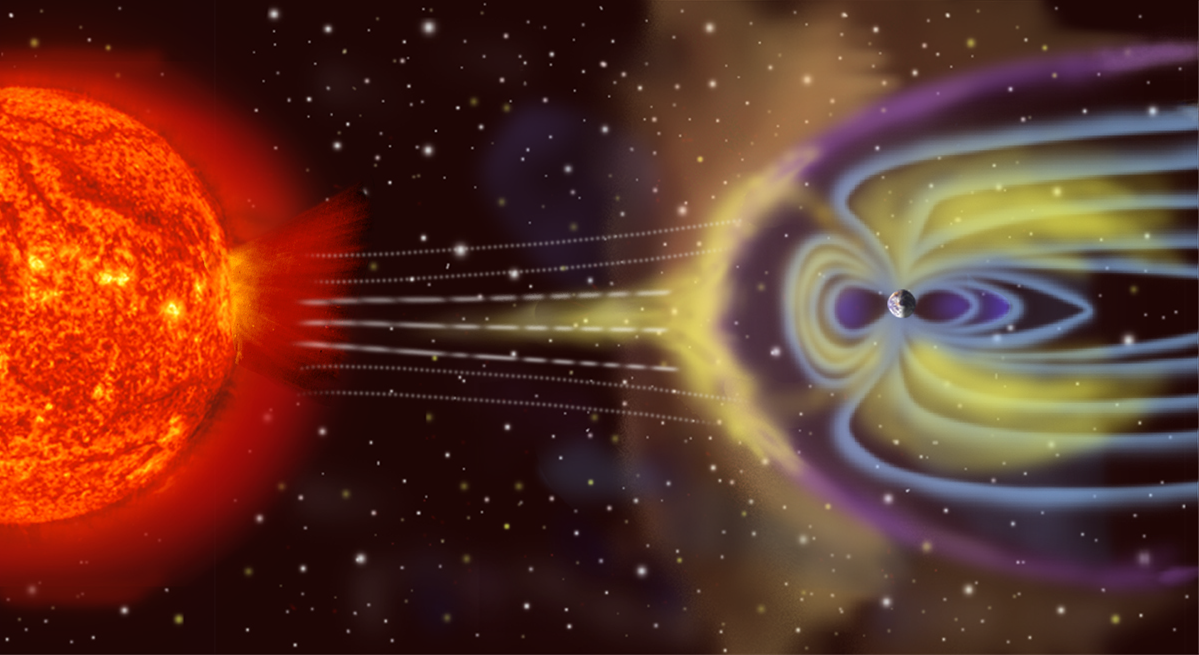
\includegraphics{./images/paste-25F555DC.png}

}

\caption{Künstlerische Darstellung der solar-terrestrischen Beziehungen}

\end{figure}

\begin{figure}

{\centering 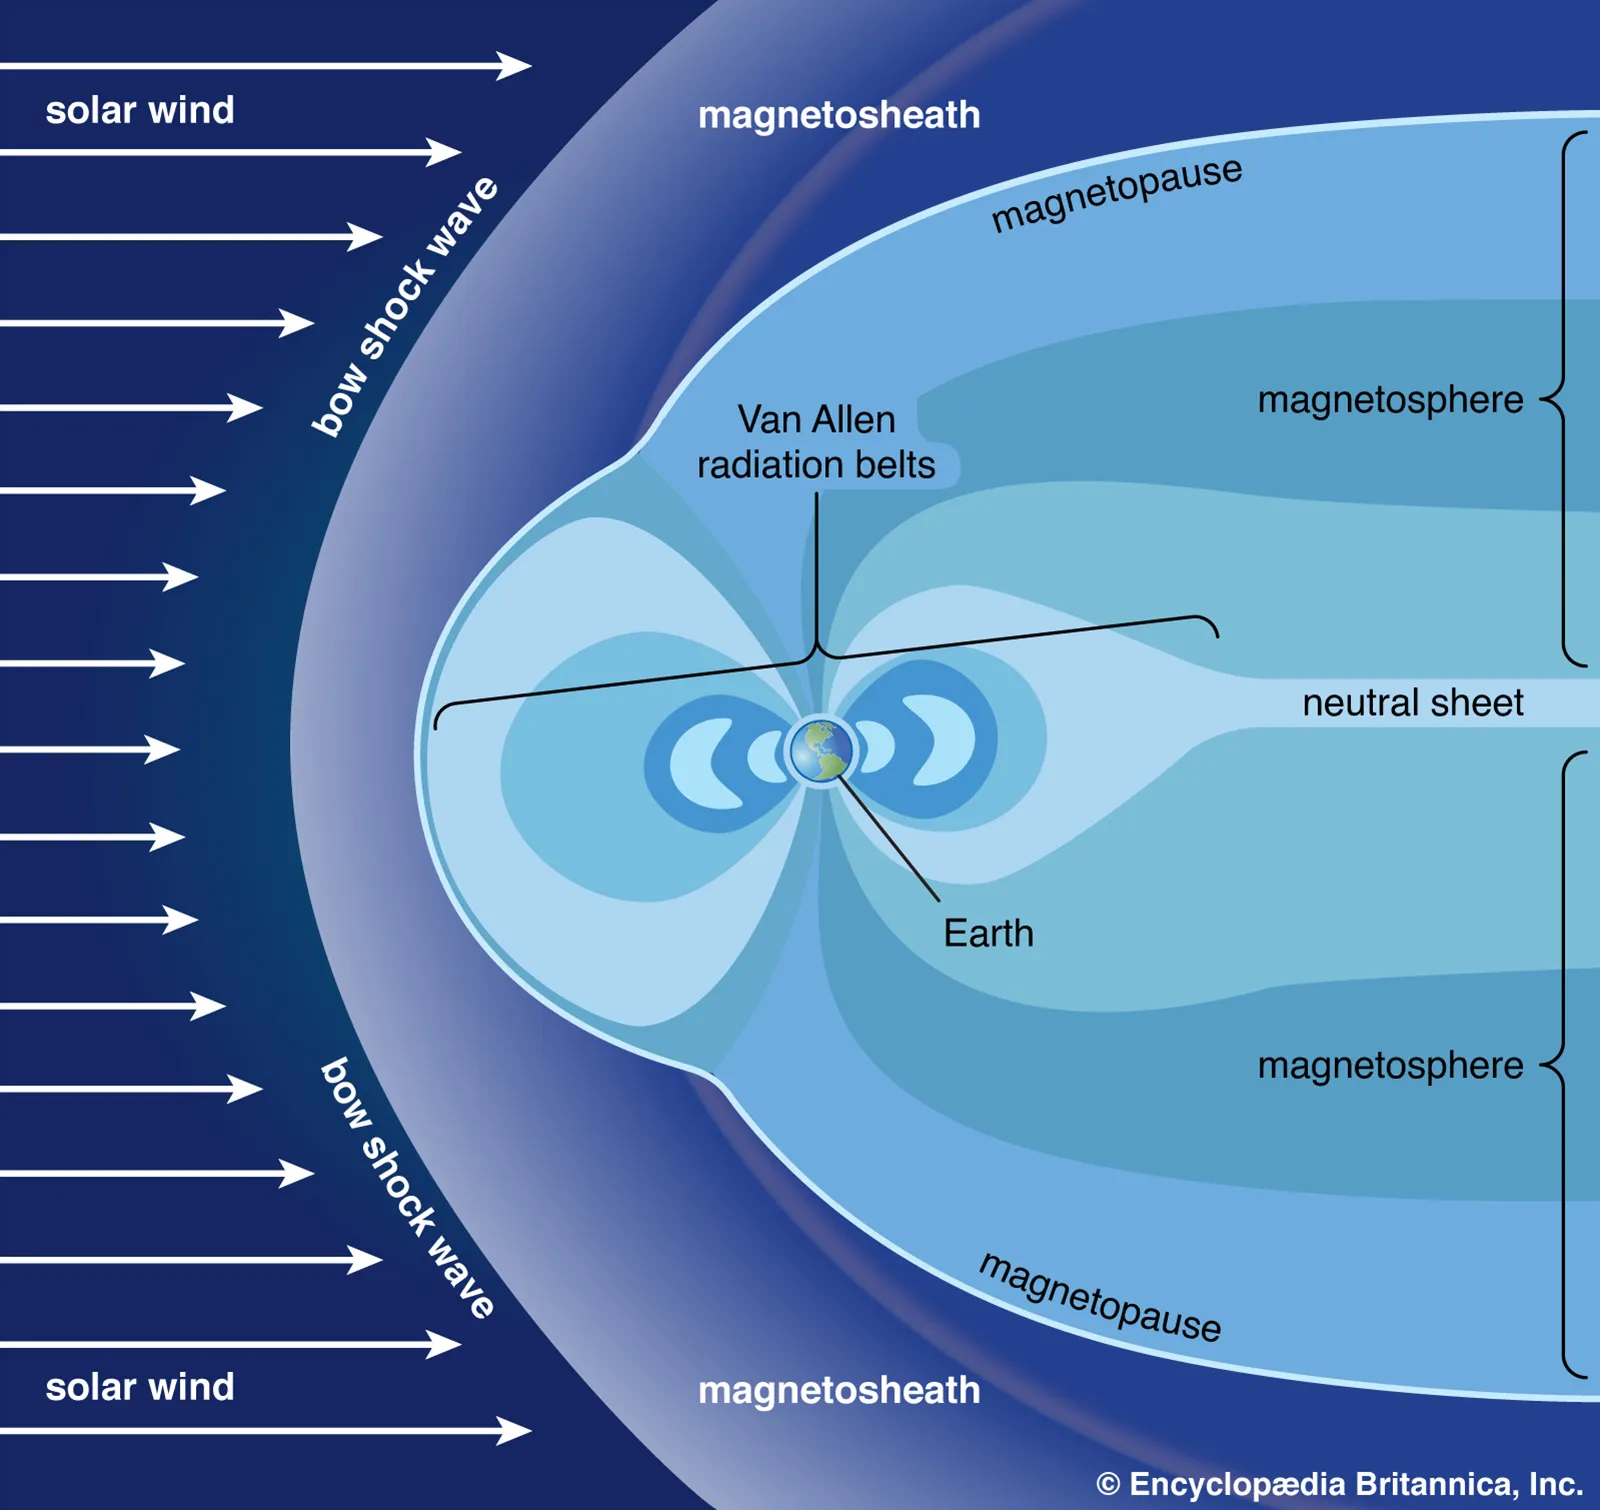
\includegraphics{./images/paste-444DBB41.png}

}

\caption{Schematische Darstellung der Magnetosphäre}

\end{figure}

In der Physik der Ionosphäre und Magnetosphäre behandeln wir Prozesse im
erdnahen Raum. Dort werden physikalische Vorgänge durch das
Erdmagnetfeld oder seine Interaktion mit dem interplanetaren Magnetfeld
bestimmt.

Eine besondere Rolle spielen hier geladene Teilchen. Wir werden sehen,
dass der erdnahe Raum nicht wirklich leer ist, sondern aus einem stark
verdünnten Gas aus geladenen und neutralen Teilchen besteht. Die
Annahme, dass im Universum Vakuum herrscht, ist falsch. Neben der
elektromagnetischen Wellenstrahlung der Sonne beobachtet man auch einen
Partikelstrom aus geladenen Teilchen. Dieses Teilchengemisch wird Plasma
genannt.

In unserem Sonnensystem findet wir Plasma beispielsweise im Sonnenwind,
der als ständiger Strom geladener Teilchen mit Geschwindigkeiten von
etwa 400 bis 600 km/s die Sonnenoberfläche verlässt.

Gelangt der Sonnenwind in den Wirkungsbereich der Magnetosphäre, werden
die geladenen Teilchen des Plasmas einer Kraft ausgesetzt, die durch das
irdische Magnetfeld hervorgerufen wird. Diese Kraft ist die
\emph{Lorentzkraft}.

Andererseits bringt die elektromagnetische Wellenstrahlung der Sonne
Energie in die Atmosphäre ein und führt zu einer höhenabhängigen
Ionisierung der Atmosphäre. Die Ionenproduktionsrate ist in der
Dynamoschicht besonders hoch. Dort besitzt die hohe Atmosphäre eine
beachtliche elektrische Leitfähigkeit. Dort bilden sich großräumige
elektrische Stromsysteme.

Die an diese Stromsysteme gekoppelten Magnetfelder können an der
Erdoberfläche gemessen werden. Da sie zeitlich variabel und großräumig
sind, eignen sich die Variationen als Energiequelle für die
Magnetotellurik. Andererseits führen Magnetfeldvariationen zu
unerwünschten Störeffekten bei geomagnetischen Messungen. Diese werden
durch Variometer erfasst und durch eine Variationskorrektur aus den
Messungen eliminiert.

Stromsysteme sind immer an bewegte Teilchenpopulationen geknüpft. Diese
können auch in der Magnetosphäre auftreten und bilden die
\emph{Van-Allen-Gürtel}. Eine kurzzeitige Erhöhung der Teilchendichte in
der Magnetosphäre, vor allem durch Koronale Massenauswürfe auf der
Sonnenoberfläche (engl. coronal mass ejection, CME), führt zur
Ausbildung von mehreren Stunden bis Tagen andauernden verstärkten
Ringströmen von einigen Erdradien Durchmesser, deren messbare
magnetische Wirkung als magnetischer Sturm bezeichnet wird.

\hypertarget{plasma}{%
\section{Plasma}\label{plasma}}

Unser Universum besteht zu 68 \% aus dunkler Energie, zu 27 \% aus
dunkler Materie und zu 5 \% aus gewöhnlicher Materie (Atomen)
(\href{https://science.nasa.gov/astrophysics/focus-areas/what-is-dark-energy/}{NASA
Science}).

Die gewöhnliche --\emph{sichtbare--} Materie besteht zu über 99.9 \% aus
Plasma.

\hypertarget{die-atmosphuxe4re-der-erde}{%
\chapter{Die Atmosphäre der Erde}\label{die-atmosphuxe4re-der-erde}}

In Kertz (1971) finden wir die folgende Gliederung der Atmosphäre
Abbildung~\ref{fig-kertz} hinsichtlich des Temperaturverlaufs, der
Homogenität sowie der Elektronendichte. Von großer Bedeutung für die
Physik der Hochatmosphäre ist der Magnetfeldeinfluss.

Unterhalb einer Höhe von 50 km befinden sich 99.9 \% der Gesamtmasse der
Atmosphäre. Die übrigen 0.1 \% verteilen sich auf ein Vielfaches des
Erdvolumens.

Die Physik der Hochatmosphäre beobachtet Vorgänge in einem stark
verdünnten Gas.

\begin{figure}

{\centering 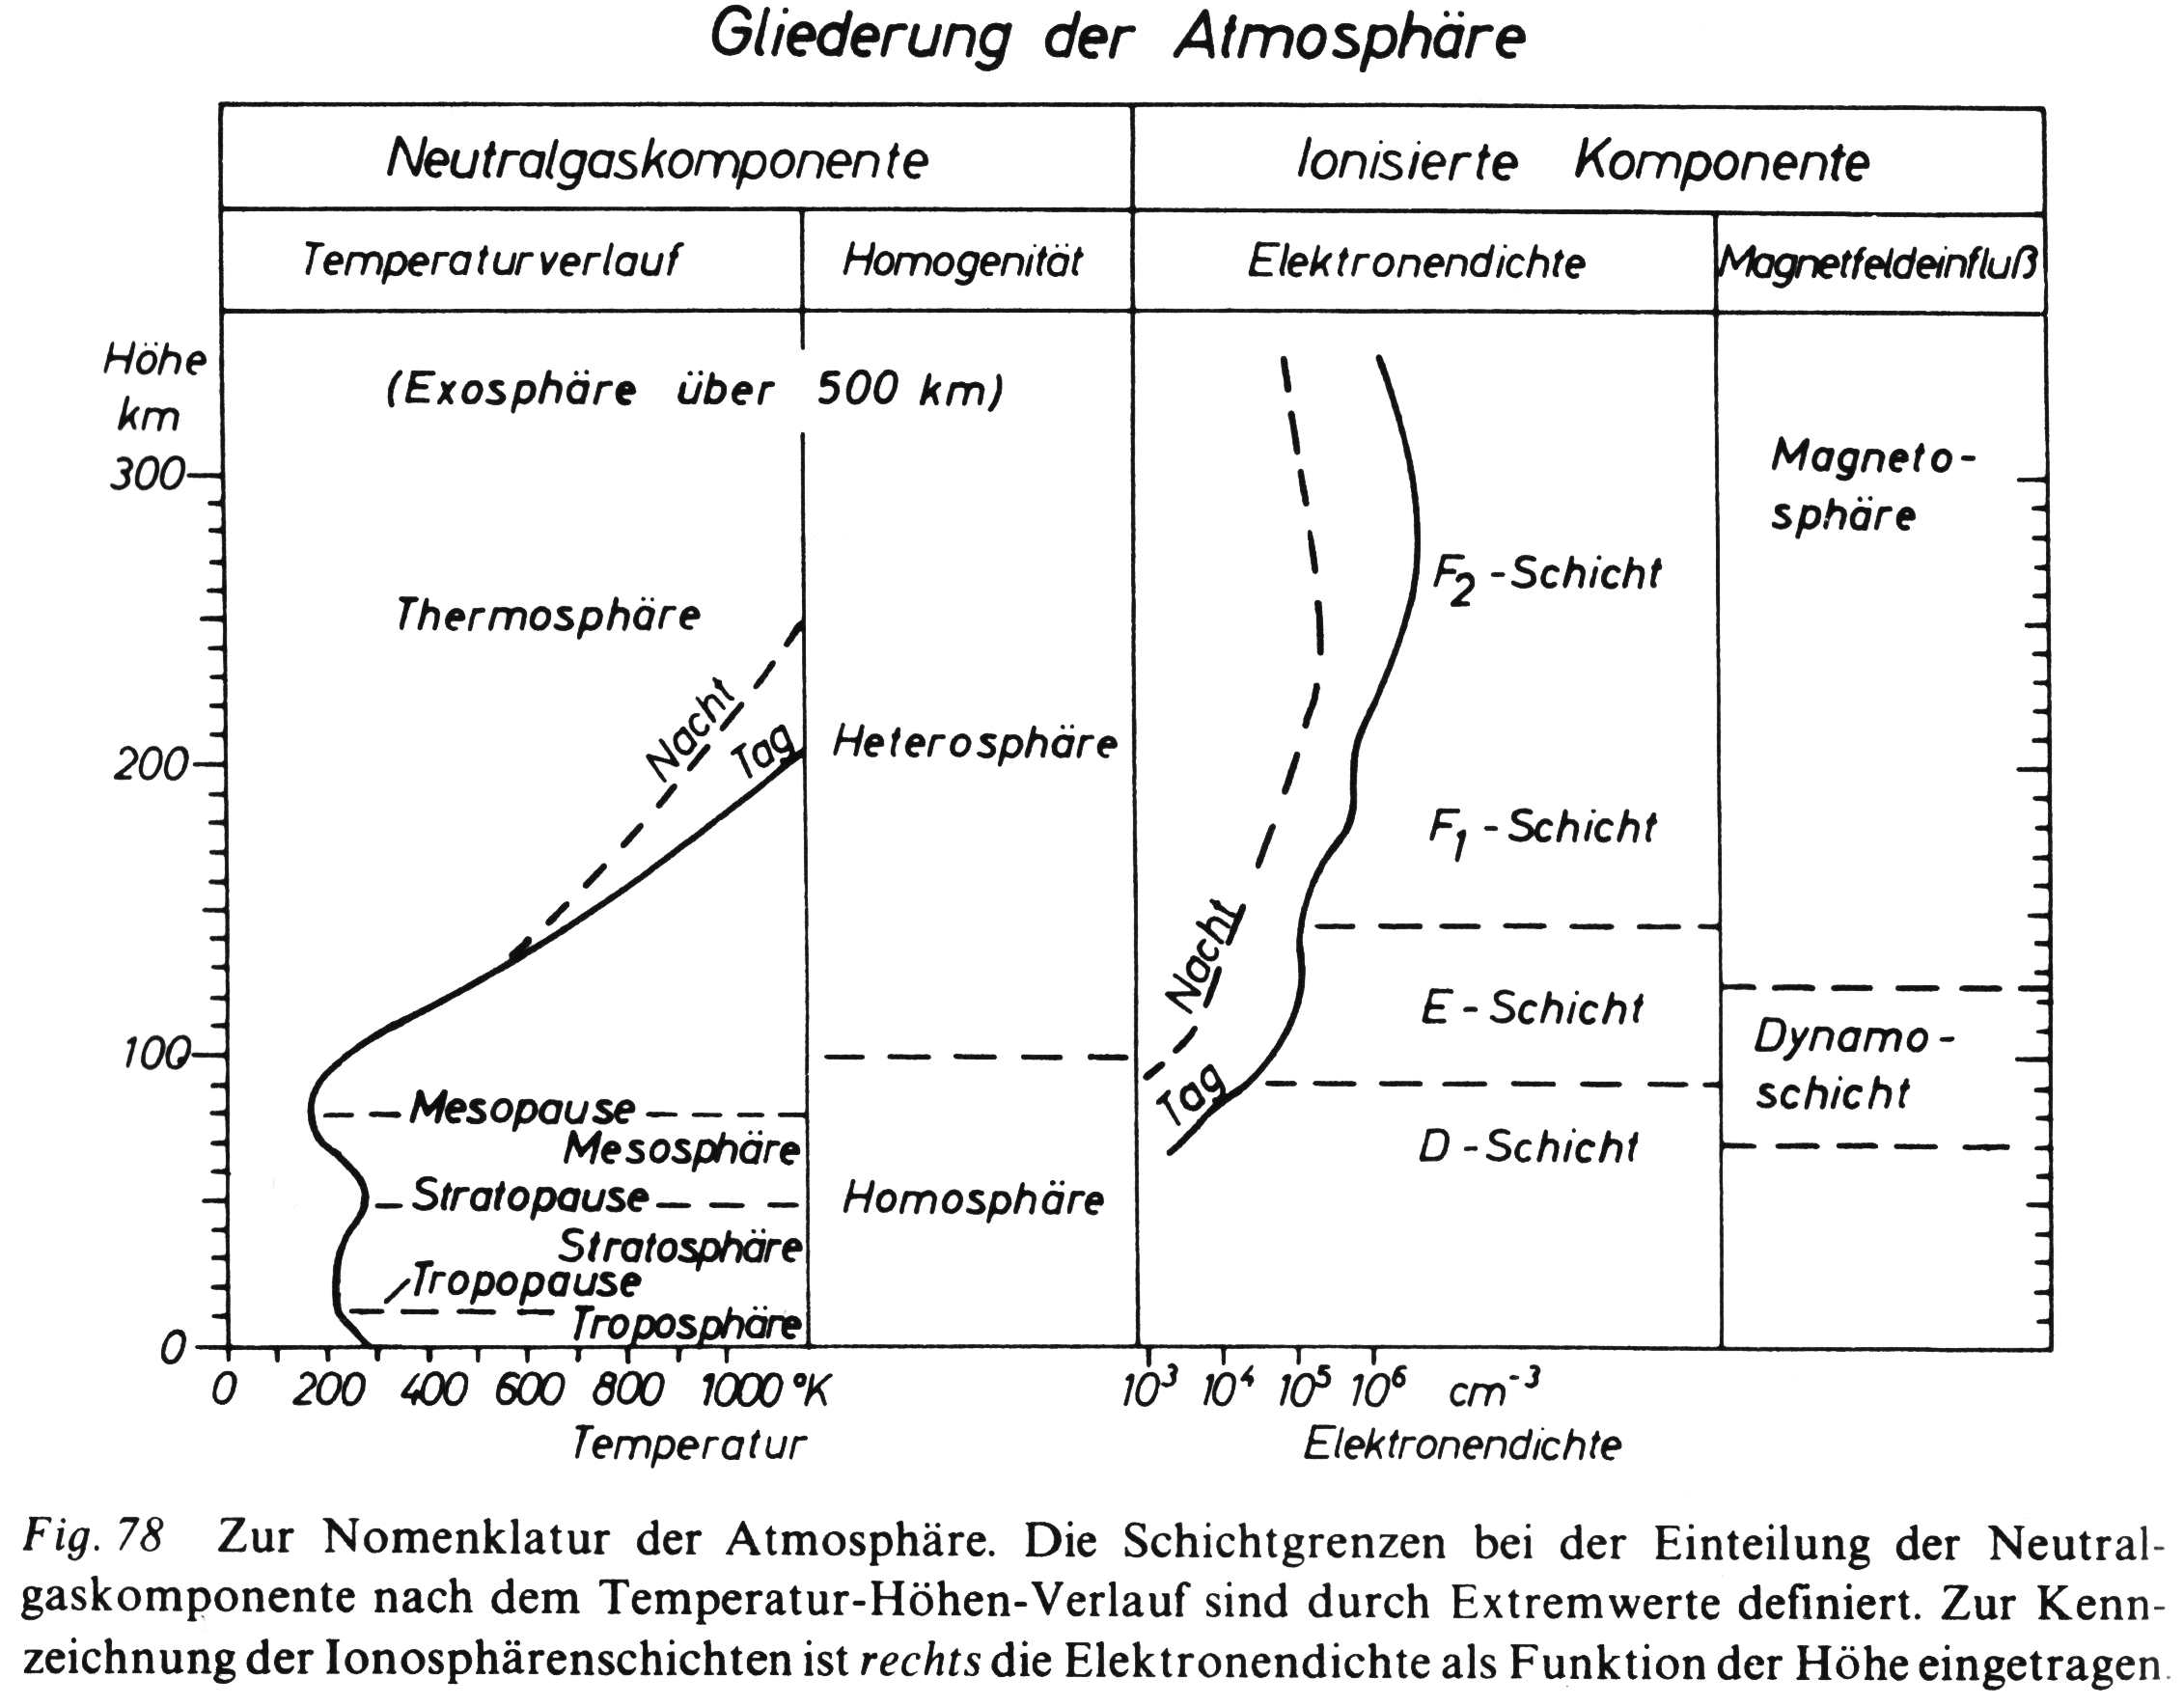
\includegraphics{./images/paste-CCE7768B.png}

}

\caption{\label{fig-kertz}Gliederung der Atmosphäre (aus Kertz)}

\end{figure}

\hypertarget{prinzipien-der-einteilung}{%
\section{Prinzipien der Einteilung}\label{prinzipien-der-einteilung}}

Die Sonnenstrahlung bewirkt eine teilweise Ionisation der Luft in der
oberen Atmosphäre. Daher ist es sinnvoll, für den ionisierten Anteil
eine andere Einteilung als für die Neutralgaskomponente zu benutzen.

\hypertarget{neutralgaskomponente}{%
\subsection{Neutralgaskomponente}\label{neutralgaskomponente}}

\hypertarget{temperaturverlauf}{%
\subsubsection{Temperaturverlauf}\label{temperaturverlauf}}

Man unterscheidet

\begin{itemize}
\tightlist
\item
  Troposphäre: Wettergeschehen, beeinflusst durch Wasser, Erdoberfläche
  und Erdrotation
\item
  Stratosphäre: Geringe vertikale Durchmischung, Strahlungsabsorption
  des Ozons führt zu Temperaturzunahme
\item
  Mesosphäre: Temperaturabnahme mit zunehmender Höhe bewirkt weniger
  starke Dichteverringerung
\item
  Thermosphäre: Ansteigende Temperatur
\end{itemize}

\hypertarget{homogenituxe4t}{%
\subsubsection{Homogenität}\label{homogenituxe4t}}

Es wird unterschieden zwischen Homo- und Heterosphäre.

In den unteren 100 km ist das Neutralgas bei konstanten
Mischungsverhältnissen als Folge von Turbulenzen gut durchmischt.

In der Heterosphäre erfolgt eine Entmischung. Mit zunehmender Höhe
treten mehr leichte Teilchen auf. In sehr großen Höhen treten wegen der
geringen Dichte keine Stöße zwischen den Teilchen auf. Die Teilchen
bewegen sich auf Keplerbahnen oder verlassen den Einflussbereich der
Erdanziehung, wenn ihre Geschwindigkeiten die Fluchtgeschwindigkeit
übersteigen. Dieser Bereich wird \emph{Exosphäre} genannt.

Die Entweichmöglichkeit besteht nur für Neutralgasteilchen. Ionisierte
Teilchen verhalten sich anders.

\hypertarget{ionisierte-komponente}{%
\subsection{Ionisierte Komponente}\label{ionisierte-komponente}}

\hypertarget{elektronendichte}{%
\subsubsection{Elektronendichte}\label{elektronendichte}}

\hypertarget{magnetfeldeinfluss}{%
\subsubsection{Magnetfeldeinfluss}\label{magnetfeldeinfluss}}

Eine etwas andere Darstellung:

\begin{figure}

{\centering 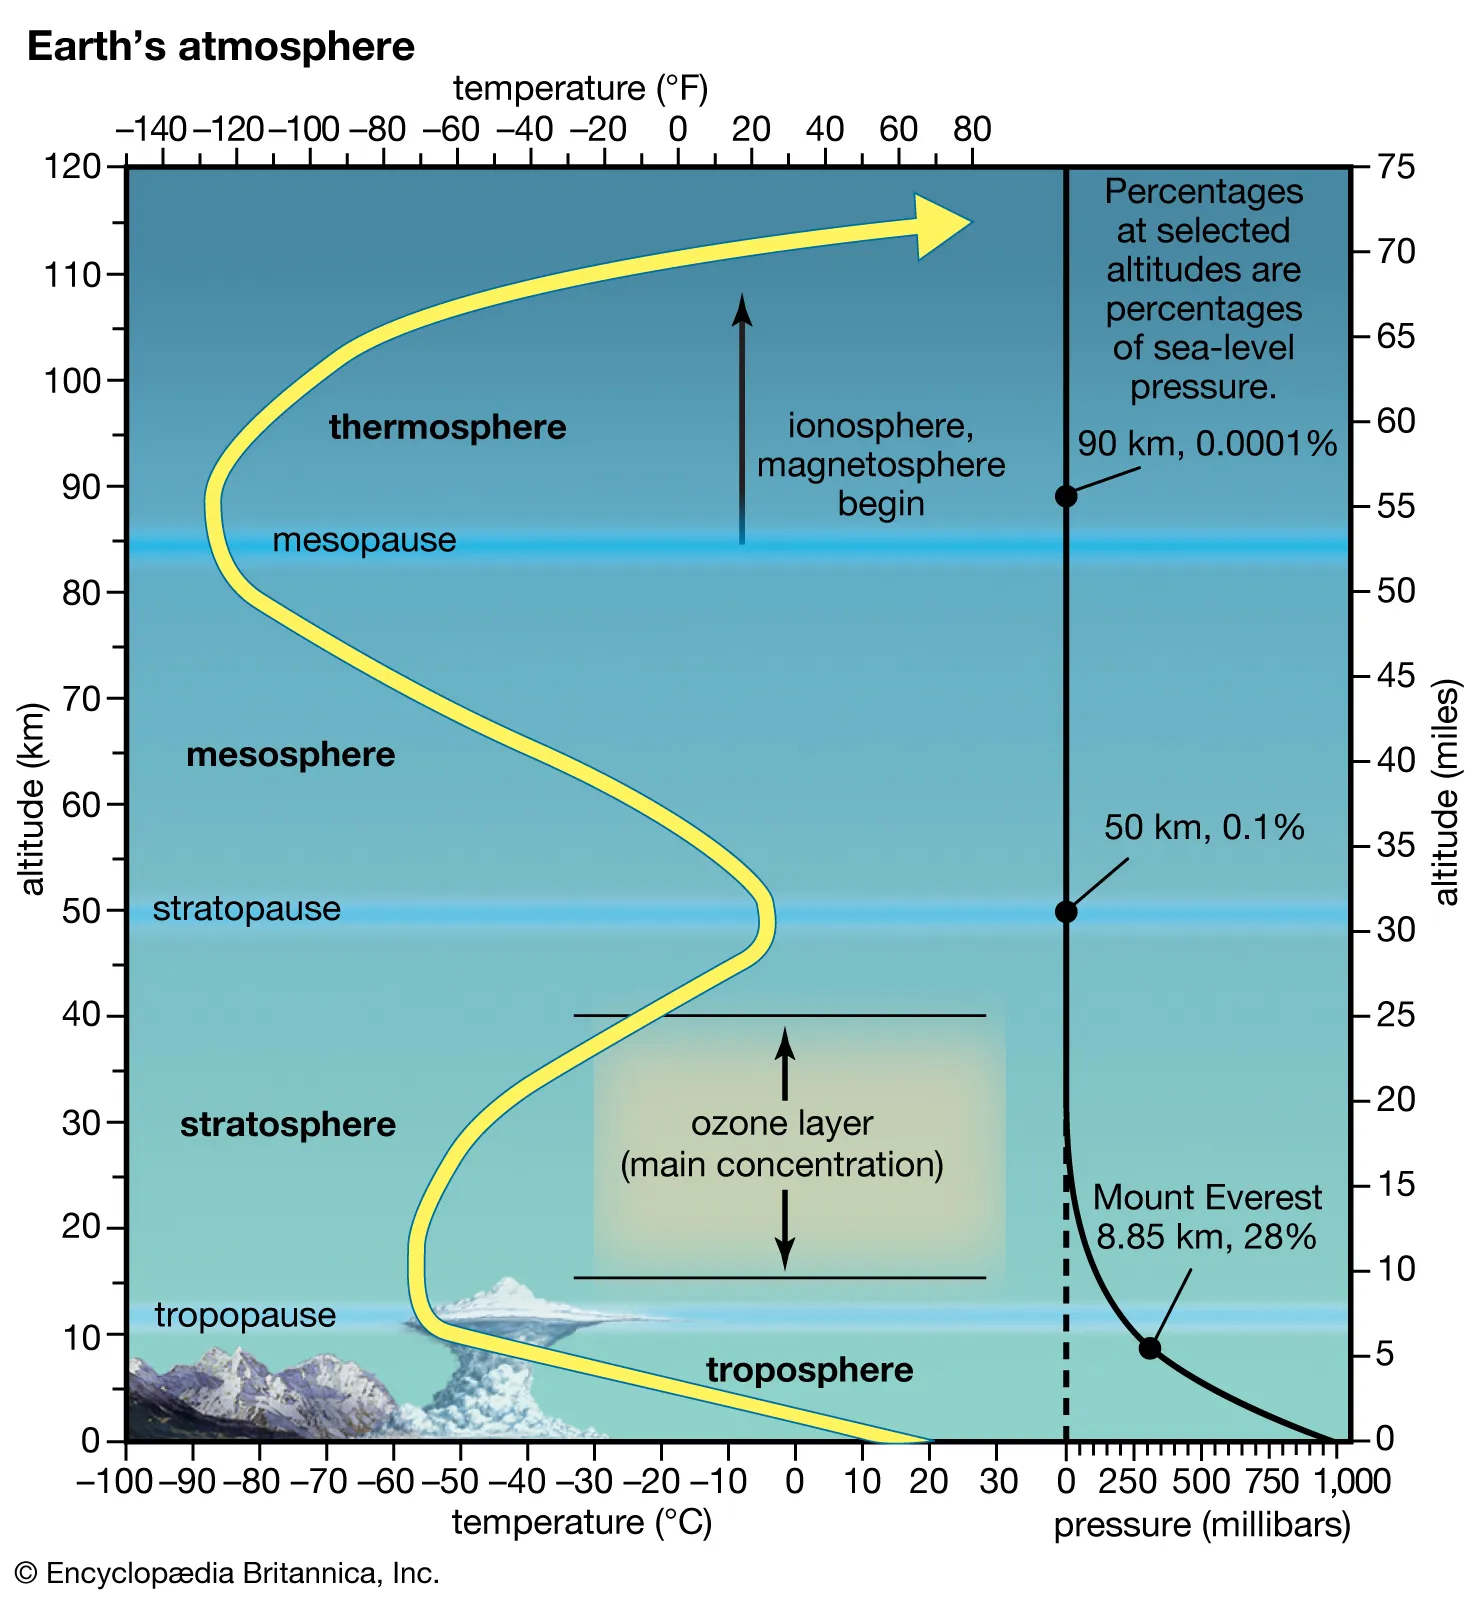
\includegraphics{./images/paste-437D2E62.png}

}

\caption{Vertikale Gliederung der Atmosphäre (aus
https://www.britannica.com/science/ionosphere-and-magnetosphere)}

\end{figure}

\hypertarget{die-grenze-zur-hochatmosphuxe4re}{%
\section{Die Grenze zur
Hochatmosphäre}\label{die-grenze-zur-hochatmosphuxe4re}}

Die Grenze zur Hochatmosphäre ist nicht einheitlich festgelegt. Sie
liegt bei \(h > 50\) km.

Warum wird diese Grenze eingeführt? Dies hat verschiedene Gründe, die
von der Methode der Erforschung der Atmosphäre, von der Zusammensetzung
der Atmosphäre sowie vom Einfluss der solaren Aktivität abhängen.

Vor allem handelt es sich um eine physikalische Einfussgrenze.

\hypertarget{methode-der-erforschung}{%
\subsection{Methode der Erforschung}\label{methode-der-erforschung}}

Registrierballons erreichen nur Höhen bis etwa 50 km, darüberhinaus sind
entweder nur Momentaufnahmen (etwa wegen der hohen Geschwindigkeit von
Forschungsraketen) oder indirekte Beobachtungen möglich.

So geben beispielsweise magnetische Aufzeichungen an der Erdoberfläche
Hinweise auf elektrische Ströme in leitfähigen Schichten der Ionosphäre.

Spektren von Polarlichtern geben Hinweise auf die chemische
Zusammensetzung.

An der Ionosphäre reflektierte Radiowellen liefern Hinweise auf die
Teilchendichte und Windbewegungen.

\hypertarget{luftchemie}{%
\subsection{Luftchemie}\label{luftchemie}}

In Höhen bis zu 50 km ist die Luft gleichmäßig durchmischt. Ihre
Zusammensetzung entspricht der an der Erdoberfläche. Oberhalb von 50 km
tritt eine höhendifferenzierte unterschiedliche Luftzusammensetzung auf,
die durch Ionisation, Dissoziation und gravitative Entmischung
verursacht wird.,

\hypertarget{steuerung-durch-solare-aktivituxe4t}{%
\subsection{Steuerung durch solare
Aktivität}\label{steuerung-durch-solare-aktivituxe4t}}

Die Dynamik der unteren Atmosphäre äußert sich in kleinskaligen und
kurzzeitigen Wettervorgängen.

Störungen der oberen Atmosphäre sind räumlich ausgedehnter und umfassen
mindestens die gesamte Tag- oder Nachtseite der Erde. Verursacht werden
sie durch Eruptionen auf der Sonne.

Im Gegensatz dazu werden die Prozesse in der unteren Atmosphäre nicht
wesentlich von der solaren Aktivität beeinflusst.

Die Grenze zwischen unterer und oberer Atmosphäre ist eine
\emph{physikalische Einflussgrenze}.

\hypertarget{aeronomie}{%
\section{Aeronomie}\label{aeronomie}}

Die Physik der Hochatmosphäre wird auch als Aeronomie bezeichnet (im
Gegensatz zur Meteorologie als Physik der unteren Atmosphäre). Die
wissenschaftliche Dachvereinigung zur Erforschung der Hochatmosphäre ist
die \href{https://www.iaga-aiga.org/}{IAGA} (International Association
of Geomagnetism and Aeronomy).

\part{Die ruhige und aktive Sonne}

\hypertarget{aufbau-der-sonne}{%
\chapter{Aufbau der Sonne}\label{aufbau-der-sonne}}

\begin{figure}

{\centering 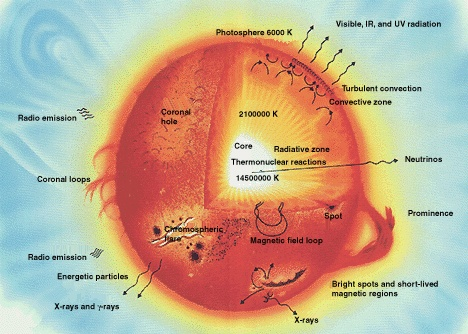
\includegraphics{./images/paste-7BD74E6D.png}

}

\caption{\label{fig-aufbau-hauptreihenstern}Aufbau eines sonnenähnlichen
Hauptreihensterns (NASA image)}

\end{figure}

\begin{figure}

{\centering 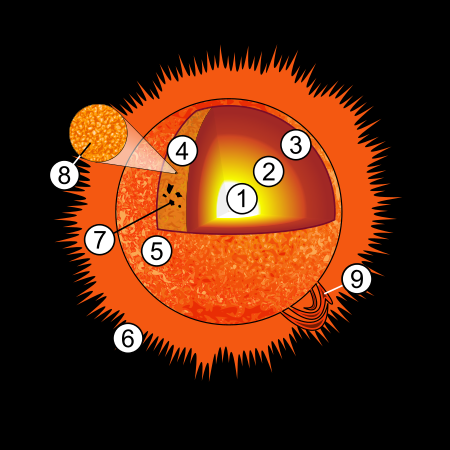
\includegraphics{./images/paste-2464B050.png}

}

\caption{\label{fig-schnitt-sonne}Schnittdiagramm der Sonne. 1-Kern,
2-Strahlunszone, 3-Konvektionszone, 4-Photosphäre, 5-Chromosphäre,
6-Corona, 7-Sonnenfleck, 8-Granulation, 9-Protuberanz (Wikipedia)}

\end{figure}

In erster Näherung ist die Sonne kugelsymmetrisch aufgebaut. Sie
befindet sich in einem stationären Gleichgewicht ohne Kontraktionen oder
Schwingungen.

Die Sonne vereint in sich etwa 99.86 \% der Masse des Sonnensystems.

Im Innern der Sonne herrscht ein hydrostatisches Gleichgewicht der nach
außen wirkenden Druckkräfte und der nach innen gerichteten
Gravitationskräfte. Es gilt

\[
\frac{d p(r)}{d r} = - f \frac{\rho(r) m(r)}{r^2}
\]

mit

\[
m(r) = 4 \pi \int_0 ^r \rho(r) r^2 \, dr
\]

\hypertarget{energiefreisetzungsprozesse}{%
\section{Energiefreisetzungsprozesse}\label{energiefreisetzungsprozesse}}

Die primäre Quelle der Sonnenenergie ist die Verschmelzung von
Wasserstoffkernen zu Heliumkernen. Dies geschieht im Kern der Sonne bei
Temperaturen von \(1.4 \times 10^7\) K.

In jeder Sekunde werden etwa 620 Millionen Tonnen Wasserstoff in Helium
umgewandelt.

\hypertarget{energietransportmechanismen}{%
\section{Energietransportmechanismen}\label{energietransportmechanismen}}

Energie gelangt nach außen durch

\begin{itemize}
\tightlist
\item
  Strahlung
\item
  Konvektion
\item
  Wärmeleitung
\end{itemize}

Benötigt wird ein Temperaturgefälle. Wärmestrom
\(\mathbf J = -k \nabla T\).

\begin{figure}

{\centering 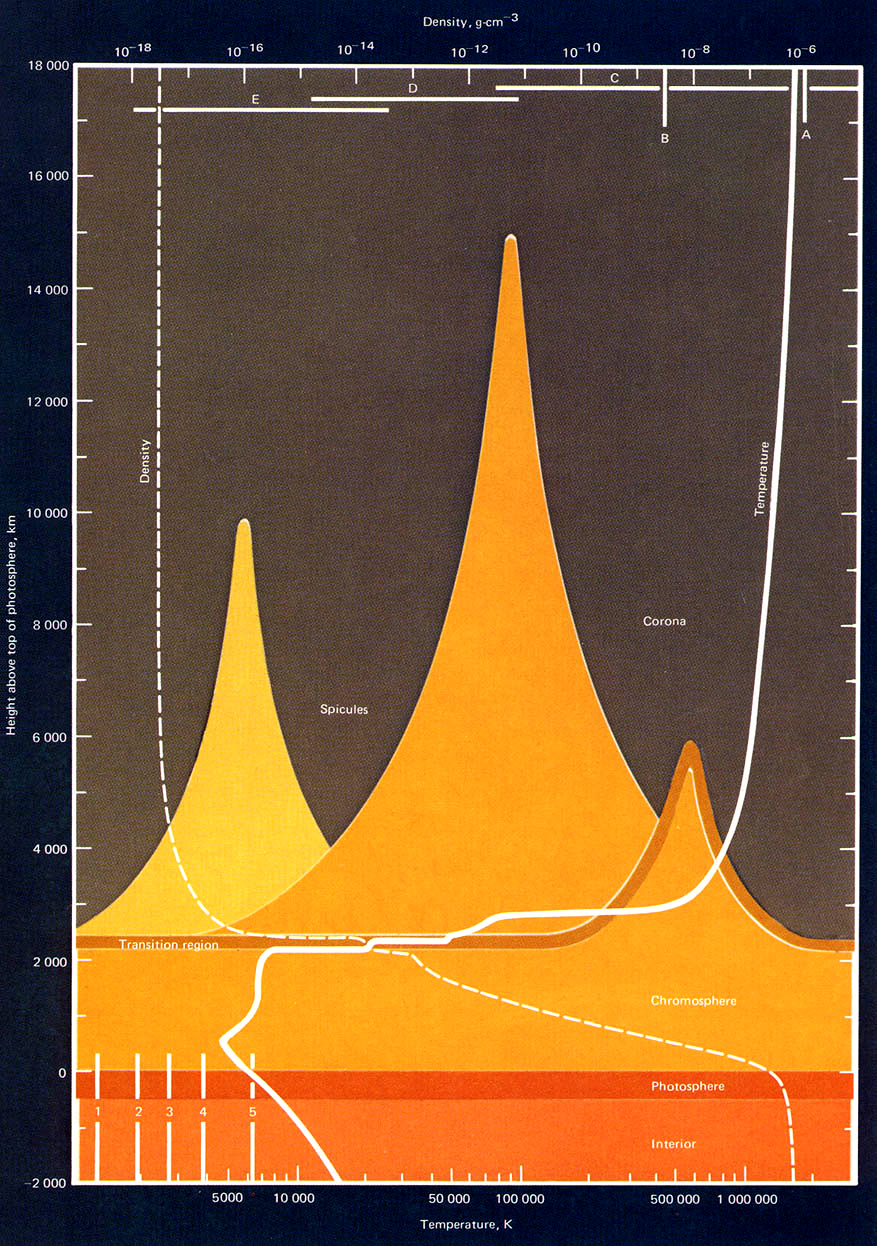
\includegraphics{./images/paste-7A6CEC06.png}

}

\caption{\label{fig-skylab}Temperatur- und Dichtemessungen von Skylab
(Quelle: Wikipedia)}

\end{figure}

\hypertarget{kern}{%
\section{Kern}\label{kern}}

Die Hälfte der Sonnenmasse konzentriert sich innerhalb von 25 \% des
Sonnenradius. Im Zentrum der Sonne beträgt der Druck 200 Milliarden bar,
die Dichte ist 150 g/cm\(^3\). Die Temperatur im Kern ist
\(15.7 \times 10^6\) K.

Nur im Kern wird thermische Energie durch Kernfusion freigesetzt. 99 \%
der Fusionsleistung von \(3.9 \times 10^{26}\) W wird innerhalb von 24
\% des Sonnenradius erzeugt. In einem Tausendstel des Volumens der Sonne
entsteht die Hälfte ihrer Leistung. Die mittlere Leistungsdichte beträgt
aber nur 140 W/m\(^3\).

Die freigesetzte Energie wird durch Strahlung nach außen transportiert.

\hypertarget{strahlungs--und-konvektionszone}{%
\section{Strahlungs- und
Konvektionszone}\label{strahlungs--und-konvektionszone}}

Ab etwa 30 \% Sonnenradius findet keine Fusion mehr statt. Wärmeenergie
wird neben der Strahlung durch Konvektion transportiert.

Ab 71 \% des Sonnenradius wird der Wärmestrom durch Konvektion
transportiert. Die Strömungsgeschwindigkeit ist mit ca. 10 m/s gering,
die Konvektionszellen sind groß und beständig (Monate bis Jahre), und
daher von Rotation und innerem Magnetfeld beeinflusst.

\hypertarget{sonnenoberfluxe4che-und-umgebung}{%
\section{Sonnenoberfläche und
Umgebung}\label{sonnenoberfluxe4che-und-umgebung}}

\hypertarget{photosphuxe4re}{%
\subsection{Photosphäre}\label{photosphuxe4re}}

Die Dichte nimmt immer schneller ab, das Material wird durchsichtig und
die Photonen können ungehindert entweichen. Am Sonnenrand sieht man
unter flacherem Beobachtungswinkel eine höhere, kältere Schicht, wodurch
der Rand dunkler erscheint.

\hypertarget{chromosphuxe4re}{%
\subsection{Chromosphäre}\label{chromosphuxe4re}}

Oberhalb der Photosphäre liegt die knapp 2000 km dicke Chromosphäre. Die
Temperatur nimmt ab, die Dichte ebenso.

\hypertarget{uxe4uuxdfere-atmosphuxe4re}{%
\section{Äußere Atmosphäre}\label{uxe4uuxdfere-atmosphuxe4re}}

\hypertarget{korona}{%
\subsection{Korona}\label{korona}}

Oberhalb der Chromosphäre befindet sich die Korona. Sie geht ohne
scharfe Grenze in den interplanetaren Raum über. Die Korona erstreckt
sich auf über ein bis zwei Sonnenradien. In der Korona regieren
Gravitation und Magnetfeld.

\hypertarget{sonnenwind}{%
\subsection{Sonnenwind}\label{sonnenwind}}

In der Korona entsteht der Sonnenwind, der mit etwa 300 km/s die Sonne
verlässt.

\hypertarget{magnetfeld}{%
\section{Magnetfeld}\label{magnetfeld}}

An der Sonnenoberfläche lässt sich das Magnetfeld wegen des
Zeeman-Effekts aus spektroskopischen Beobachtungen feststellen.
Spektrallinien spalten sich bei Anwesenheit eines Magnetfeldes auf. Der
Spektrallinienabstand ist proportional zur Feldstärke.

Die Feldstärke im Umfeld von Sonnenflecken beträgt bis zu 0.4 T.

Das großräumige Magnetfeld lässt sich nur grob durch ein Dipolfeld
beschreiben. An der Sonnenoberfläche ist die Feldstärke mit etwa 100,000
nT nur etwa doppelt so groß wie das der Erde auf der Erdoberfläche.

\hypertarget{differentielle-rotation}{%
\section{Differentielle Rotation}\label{differentielle-rotation}}

Die Strahlungszone rotiert gleichförmig mit einer Periode von knapp 27
Tagen (Frequenz etwa 430 nHz, s. Abb. Abbildung~\ref{fig-diffrot}) bis
zur Tachokline, der Übergangszone zur differentiell rotierenden
Konvektionszone.

\begin{figure}

{\centering 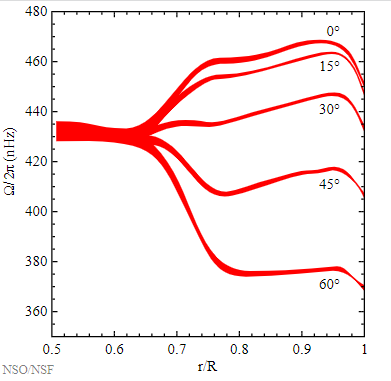
\includegraphics{./images/paste-A039882F.png}

}

\caption{\label{fig-diffrot}Radialer Verlauf der Sonnenrotation für
verschiedene heliographische Breiten. Ausgehend von der differentiell
rotierenden Oberfläche steigt in den oberen 4 \% die
Winkelgeschwindigkeit steil an, um dann bis zur tachoklinen Region
leicht abzufallen. Dort gleicht sie sich an die der nahezu starr
rotierenden Strahlungszone an (Quelle: Wikipedia).}

\end{figure}

\hypertarget{die-sonne-als-energiequelle}{%
\chapter{Die Sonne als
Energiequelle}\label{die-sonne-als-energiequelle}}

Die Erde umkreist die Sonne in einer annähernd kreisförmigen Umlaufbahn
mit Radius 1 AU = \(1.495978707 \times 10^{8}\) km.

Die Sonne besitzt eine Strahlungsleistung (``Leuchtkraft'') von
\(3.828 \times 10^{26}\) W.

Die scheinbare Größe der Erde aus der Sicht der Sonne beträgt ca. 18
Bogensekunden.

Der Raumwinkel \(\Omega\), unter dem die Erde erscheint, beträgt etwa
\(5.7\times 10^{-9}\) sr, damit emittiert die Sonne insgesamt etwa das
\(2.2\times 10^9\)-fache der Strahlung, die lediglich auf die Fläche der
Erde entfällt.

Berechnung der scheinbaren Größe:

\[
\alpha = 2 \arctan \left( \frac{R}{d} \right)
\]

Berechnung des kanonischen Raumwinkels \(\Omega\) eines Kegels mit
Öffnungswinkel \(2\theta = \alpha\):

\[
\Omega = \int_0^{2 \pi} \mathrm d\phi \int_0^\theta \sin\theta' \mathrm d\theta' =  2 \pi \left( 1 - \cos\theta \right)
\]

\begin{Shaded}
\begin{Highlighting}[]
\ImportTok{using} \BuiltInTok{Markdown}
\NormalTok{R\_E }\OperatorTok{=} \FloatTok{6.3781e6}\NormalTok{;}
\NormalTok{AU }\OperatorTok{=} \FloatTok{1.495978707e11}\NormalTok{;}
\NormalTok{alpha }\OperatorTok{=} \FloatTok{2} \OperatorTok{*} \FunctionTok{atan}\NormalTok{(R\_E }\OperatorTok{/}\NormalTok{ AU);}
\NormalTok{bs }\OperatorTok{=}\NormalTok{ alpha }\OperatorTok{*} \FloatTok{180} \OperatorTok{/} \ConstantTok{pi} \OperatorTok{*} \FloatTok{3600}\NormalTok{;}
\NormalTok{Omega }\OperatorTok{=} \FloatTok{2} \OperatorTok{*} \ConstantTok{pi} \OperatorTok{*}\NormalTok{ (}\FloatTok{1} \OperatorTok{{-}} \FunctionTok{cos}\NormalTok{(alpha }\OperatorTok{/} \FloatTok{2}\NormalTok{));}
\NormalTok{Markdown.}\FunctionTok{parse}\NormalTok{(}\StringTok{"""}
\StringTok{Die scheinbare Größe beträgt }\SpecialCharTok{$}\NormalTok{(}\FunctionTok{round}\NormalTok{(bs, digits}\OperatorTok{=}\FloatTok{2}\NormalTok{))}\StringTok{ Bogensekunden.}

\StringTok{Der Raumwinkel beträgt }\SpecialCharTok{$}\NormalTok{(}\FunctionTok{round}\NormalTok{(Omega, sigdigits}\OperatorTok{=}\FloatTok{2}\NormalTok{))}\StringTok{ sr.}

\StringTok{Die Sonne emittiert das }\SpecialCharTok{$}\NormalTok{(}\FunctionTok{round}\NormalTok{(}\FloatTok{4} \OperatorTok{*} \ConstantTok{pi} \OperatorTok{/}\NormalTok{ Omega, sigdigits}\OperatorTok{=}\FloatTok{2}\NormalTok{))}\StringTok{{-}fache bezogen auf die Erdscheibe.}
\StringTok{"""}\NormalTok{)}
\CommentTok{\# println("Der Raumwinkel beträgt $(round(Omega, sigdigits=2)) sr.")}
\CommentTok{\# println("Die Sonne emittiert das $(round(4 * pi / Omega, sigdigits=2)){-}fache bezogen auf die Erdscheibe.")}
\end{Highlighting}
\end{Shaded}

Die scheinbare Größe beträgt 17.59 Bogensekunden.

Der Raumwinkel beträgt 5.7e-9 sr.

Die Sonne emittiert das 2.2e9-fache bezogen auf die Erdscheibe.

\hypertarget{solarkonstante}{%
\section{Solarkonstante}\label{solarkonstante}}

\begin{Shaded}
\begin{Highlighting}[]
\NormalTok{S }\OperatorTok{=} \FloatTok{3.828e26} \OperatorTok{/} \FloatTok{4} \OperatorTok{/} \ConstantTok{pi} \OperatorTok{/}\NormalTok{ AU}\OperatorTok{\^{}}\FloatTok{2}\NormalTok{;}
\NormalTok{Markdown.}\FunctionTok{parse}\NormalTok{(}\StringTok{"""}
\StringTok{Die Leuchtkraft der Sonne verteilt sich gleichmäßig (isotrop) auf einer Kugeloberfläche. In der Entfernung von 1 AU ergibt sich daraus die Solarkonstante rechnerisch zu}

\StringTok{\textasciigrave{}\textasciigrave{}S = \textasciigrave{}\textasciigrave{} }\SpecialCharTok{$}\NormalTok{(}\FunctionTok{round}\NormalTok{(S, digits}\OperatorTok{=}\FloatTok{2}\NormalTok{))}\StringTok{ W/m\textasciigrave{}\textasciigrave{}\^{}2\textasciigrave{}\textasciigrave{}.}
\StringTok{"""}\NormalTok{)}
\end{Highlighting}
\end{Shaded}

Die Leuchtkraft der Sonne verteilt sich gleichmäßig (isotrop) auf einer
Kugeloberfläche. In der Entfernung von 1 AU ergibt sich daraus die
Solarkonstante rechnerisch zu

\(S =\) 1361.17 W/m\(^2\).

Der über Satellitenmessungen bestimmte Wert ist \(S=1361\) W/m\(^{2}\).

Die Verteilung von Kontinenten und Ozeanen auf der Erdoberfläche führt
zur Absorption und unvollständigen Rückstrahlung der Sonneneinstrahlung.
Das Rückstrahlvermögen oder die Albedo der Erde ist 0.3, damit beträgt
die Absorption 0.7.

Mit der experimentell bestimmten Solarkonstante können wir zwei Größen
abschätzen:

\begin{itemize}
\tightlist
\item
  Temperatur auf der Erdoberfläche ohne Einfluss der Atmosphäre
\item
  effektive Oberflächentemperatur eines der Sonne äquivalenten schwarzen
  Strahlers.
\end{itemize}

\hypertarget{temperatur-auf-der-erdoberfluxe4che}{%
\subsection{Temperatur auf der
Erdoberfläche}\label{temperatur-auf-der-erdoberfluxe4che}}

Wir benutzen das Stefan-Boltzmann-Gesetz, um die Oberflächentemperatur
der Erde ohne Berücksichtigung der Atmosphäre zu berechnen.

\hypertarget{stefan-boltzmann-gesetz}{%
\subsubsection{Stefan-Boltzmann-Gesetz}\label{stefan-boltzmann-gesetz}}

Das Stefan-Boltzmann-Gesetz gibt an, welche Strahlungsleistung \(P\) ein
schwarzer Körper der Fläche \(A\) und der absoluten Temperatur \(T\)
aussendet. Es lautet

\[
P = \sigma\, A \, T^4
\] mit der Stefan-Boltzmann-Konstanten

\[
\sigma = 5.670374419 \times 10^{-8}~W\cdot m^{-2} K^{-4}
\] Zur Lösung des Problems stellen wir eine Strahlungsbilanz auf, wonach
die Sonneneinstrahlung auf der Erdoberfläche gleich der Abstrahlung in
den Kosmos ist.

Mit der oben angegeben Absorption von 0.7 gilt für die Einstrahlung auf
der als Kreisscheibe angenommenen Erdoberfläche

\[
P_{in} = 0.7 \, S \, \pi R_E^2
\]

\begin{Shaded}
\begin{Highlighting}[]
\NormalTok{Markdown.}\FunctionTok{parse}\NormalTok{(}\StringTok{"""}
\StringTok{Die Einstrahlung beträgt bei vollständiger Absorption dagegen}
\SpecialCharTok{$}\NormalTok{(}\FunctionTok{round}\NormalTok{(S }\OperatorTok{*} \ConstantTok{pi} \OperatorTok{*}\NormalTok{ R\_E}\OperatorTok{\^{}}\FloatTok{2} \OperatorTok{*} \FloatTok{1e{-}15}\NormalTok{, digits}\OperatorTok{=}\FloatTok{3}\NormalTok{))}\StringTok{ PW.}
\StringTok{"""}\NormalTok{)}
\end{Highlighting}
\end{Shaded}

Die Einstrahlung beträgt bei vollständiger Absorption dagegen 173.958
PW.

Die Einstrahlung beträgt also etwa 174 Petawatt! Die aktuell
leistungsfähigsten Laser (LLNL (USA): ``Nova Laser'', 2012; Osaka Univ.
(Japan): ``LFEX'', 2015; EU: ``ELI-NP'', 2015) erreichten kurzzeitig
1.25, 2 bzw. 10 PW für 0.5, 1 bzw. \textless{} 0.01 Pikosekunden (1
Pikosekunde = 10\(^{-12}\) s), was einer Energie von 600, 2000 bzw. 10 J
entspricht.

Die Abstrahlung in den Kosmos ist \[
P_{out} = \sigma 4 \pi R_E^2 T^4
\] Daraus ermitteln wir die Oberflächentemperatur eines äquivalenten
schwarzen Strahlers. Sie lautet \[
T = \sqrt[4]{\frac{0.7 S}{4 \sigma}}
\]

\begin{Shaded}
\begin{Highlighting}[]
\NormalTok{S }\OperatorTok{=} \FloatTok{1361}\NormalTok{;}
\NormalTok{sigma }\OperatorTok{=} \FloatTok{5.670374419e{-}8}\NormalTok{;}
\NormalTok{T }\OperatorTok{=}\NormalTok{ (}\FloatTok{0.7} \OperatorTok{*}\NormalTok{ S }\OperatorTok{/} \FloatTok{4}  \OperatorTok{/}\NormalTok{sigma)}\OperatorTok{\^{}}\FloatTok{0.25} \OperatorTok{{-}} \FloatTok{273.15}\NormalTok{;}
\NormalTok{Markdown.}\FunctionTok{parse}\NormalTok{(}\StringTok{"""}
\StringTok{Die Oberflächentemperatur auf der Erde beträgt ohne Atmosphäre T = }\SpecialCharTok{$}\NormalTok{(}\FunctionTok{round}\NormalTok{(T, digits}\OperatorTok{=}\FloatTok{1}\NormalTok{))}\StringTok{ °C.}
\StringTok{"""}\NormalTok{)}
\end{Highlighting}
\end{Shaded}

Die Oberflächentemperatur auf der Erde beträgt ohne Atmosphäre T = -18.6
°C.

Somit ergibt sich für die Erde eine Temperatur von ca. -18 °C, die
allein verursacht durch die Sonneneinstrahlung, jedoch ohne
Berücksichtigung des Einflusses der Atmosphäre (Treibhauseffekt) auf der
Erdoberfläche herrschen würde. In der Realität misst man dort eine
deutlich höhere Temperatur von im Mittel ca. 14 °C. Die Differenz von 32
K wird durch den Treibhauseffekt verursacht.

\hypertarget{effektive-oberfluxe4chentemperatur-der-sonne}{%
\subsection{Effektive Oberflächentemperatur der
Sonne}\label{effektive-oberfluxe4chentemperatur-der-sonne}}

Ebenso lässt sich mit Hilfe des Stefan-Boltzmann-Gesetzes aus den oben
gegebenen Werten die effektive Oberflächentemperatur der Sonne
errechnen.

Der Radius der Sonne beträgt \(R_S = 6.963 \times 10^8\) m. Ihre
Leuchtkraft lässt sich über die Solarkonstante \(S\) und den Radius
\(d\) der Erdumlaufbahn angeben. Es gilt \[
P_{out} = 4 \pi d^2 \, S
\] Die Fläche des angenommenen schwarzen Strahlers ist \[
A = 4 \pi R_S^2
\]

Die Temperatur auf der Sonnenoberfläche ist demnach \[
T = \sqrt[4]{\frac{P_{out}}{\sigma A}}
\]

Wir setzen ein und erhalten

\begin{Shaded}
\begin{Highlighting}[]
\NormalTok{P\_out }\OperatorTok{=} \FloatTok{4} \OperatorTok{*} \ConstantTok{pi} \OperatorTok{*}\NormalTok{ AU}\OperatorTok{\^{}}\FloatTok{2} \OperatorTok{*}\NormalTok{ S;}
\NormalTok{R\_S }\OperatorTok{=} \FloatTok{6.96342e8}\NormalTok{;}
\NormalTok{A }\OperatorTok{=} \FloatTok{4} \OperatorTok{*} \ConstantTok{pi} \OperatorTok{*}\NormalTok{ R\_S}\OperatorTok{\^{}}\FloatTok{2}\NormalTok{;}
\NormalTok{T }\OperatorTok{=}\NormalTok{ (P\_out }\OperatorTok{/}\NormalTok{ sigma }\OperatorTok{/}\NormalTok{ A)}\OperatorTok{\^{}}\FloatTok{0.25}\NormalTok{;}
\NormalTok{Markdown.}\FunctionTok{parse}\NormalTok{(}\StringTok{"""}
\StringTok{Die effektive Temperatur der Sonne ist T = }\SpecialCharTok{$}\NormalTok{(}\FunctionTok{round}\NormalTok{(T, digits}\OperatorTok{=}\FloatTok{2}\NormalTok{))}\StringTok{ K.}
\StringTok{"""}\NormalTok{)}
\end{Highlighting}
\end{Shaded}

Die effektive Temperatur der Sonne ist T = 5769.17 K.

Die Temperatur, die ein gleich großer schwarzer Strahler haben müsste,
um die gleiche Strahlung abzugeben, beträgt also etwa 5770 K.

\hypertarget{treibhausgase}{%
\section{Treibhausgase}\label{treibhausgase}}

\hypertarget{sonnenflecken}{%
\chapter{Sonnenflecken}\label{sonnenflecken}}

Sonnenflecken sind dunkle Stellen auf der Sonnenoberfläche. Sie sind
kühler und strahlen weniger sichtbares Licht ab als der Rest der
Sonnenoberfläche.

Sonnenflecken bilden das einfachste Maß für die Sonnenaktivität.

Die Häufigkeit der Sonnenflecken unterliegt einer Periodizität von
durchschnittlich 11 Jahren.

Ursache der Sonnenflecken sind starke Magnetfelder, welche den
Wärmetransport an die Sonnenoberfläche behindern.

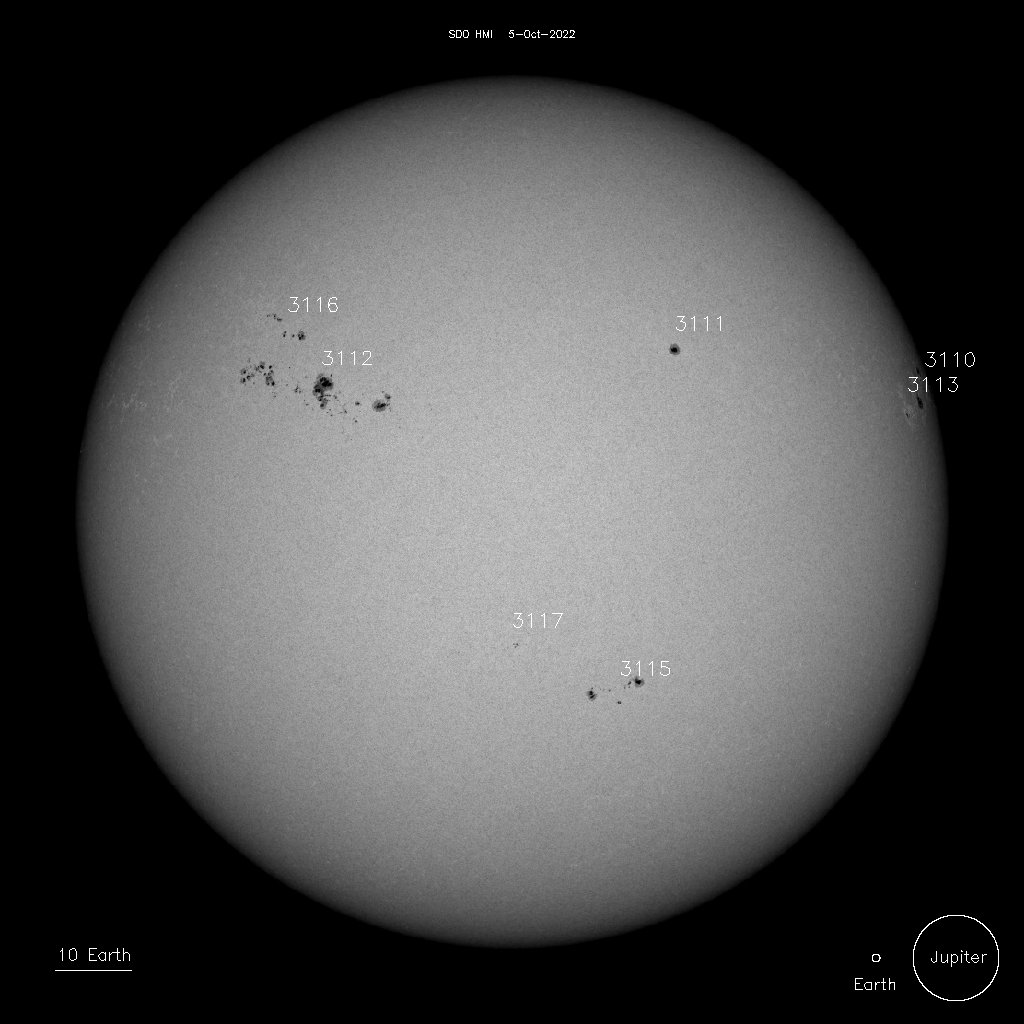
\includegraphics{./images/paste-612C7829.png}

Die Häufigkeit der Sonnenflecken wird durch die Relativzahl erfasst.

man zählt die Einzelflecken (Zahl \(f\)) und addiert dazu das Zehnfache
der Gruppenanzahl (Zahl \(g\)).

Die Sonnenfleckenrelativzahl ist eine Maßzahl der Sonnenaktivität und
berechnet sich aus

\[
R = k ( f + 10 g)
\]

wobei \(k\) ein vom Beobachter und seinen Instrumenten abhängiger
Korrekturfaktor ist.

\hypertarget{aufzeichnungen-der-sonnenfleckenrelativzahl}{%
\section{Aufzeichnungen der
Sonnenfleckenrelativzahl}\label{aufzeichnungen-der-sonnenfleckenrelativzahl}}

Zuständig für die Berechnung, Speicherung und Verbreitung der
Sonnenfleckenrelativzahl ist das
\href{https://www.sidc.be/silso/home}{Solar Influences Data analysis
Center (SIDC)}.

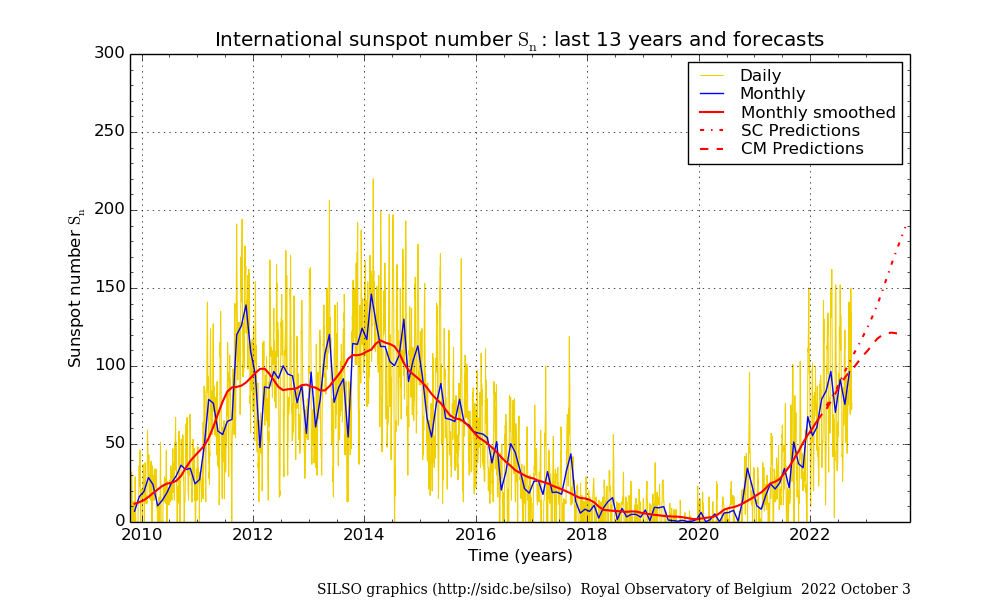
\includegraphics{./images/paste-F8C5D725.png}

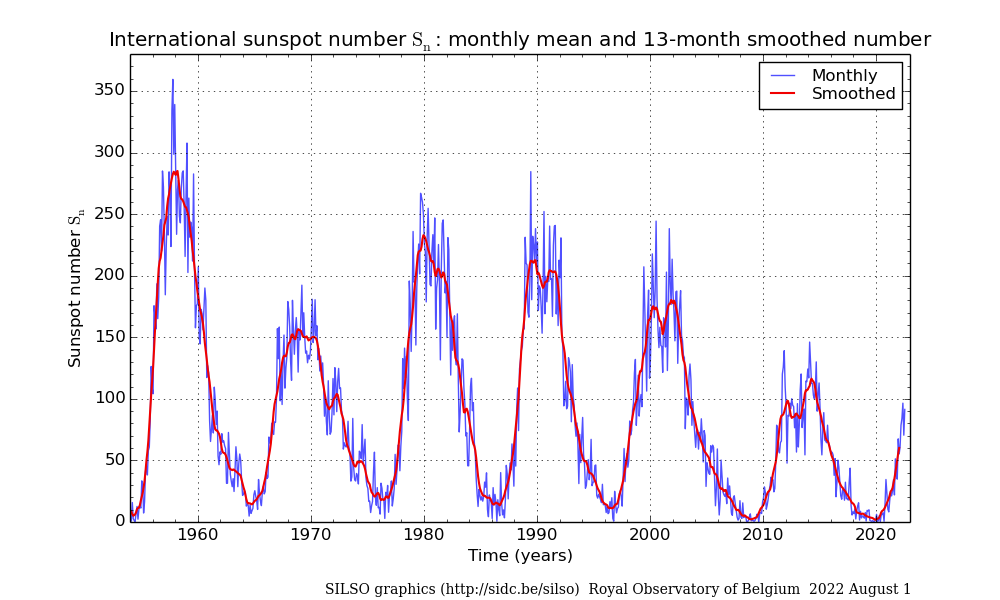
\includegraphics{./images/paste-DE59FE1D.png}

Wir wollen nun die aktuellen Daten visualisieren und analysieren. dazu
nutzen wir einenDatensatz der Monatsmittelwerte der
Sonnenfleckenrelativzahl von 1749 bis heute.

\begin{Shaded}
\begin{Highlighting}[]
\ImportTok{using} \BuiltInTok{DataFrames}
\ImportTok{using} \BuiltInTok{CSV}
\ImportTok{using} \BuiltInTok{Plots}
\FunctionTok{theme}\NormalTok{(}\OperatorTok{:}\NormalTok{vibrant)}
\FunctionTok{default}\NormalTok{(frame\_style}\OperatorTok{=:}\NormalTok{box)}
\NormalTok{df }\OperatorTok{=}\NormalTok{ CSV.}\FunctionTok{read}\NormalTok{(}\StringTok{"SN\_m\_tot\_V2.0.csv"}\NormalTok{, delim}\OperatorTok{=}\StringTok{";"}\NormalTok{, header}\OperatorTok{=}\FloatTok{1}\NormalTok{,  DataFrame)}
\NormalTok{t }\OperatorTok{=}\NormalTok{ df[}\OperatorTok{:}\NormalTok{, }\OperatorTok{:}\NormalTok{FracOfYear]}
\NormalTok{SN }\OperatorTok{=}\NormalTok{ df[}\OperatorTok{:}\NormalTok{, }\OperatorTok{:}\NormalTok{SN]}
\FunctionTok{plot}\NormalTok{(t, SN, label}\OperatorTok{=}\StringTok{""}\NormalTok{)}
\FunctionTok{xlabel!}\NormalTok{(}\StringTok{"Jahr"}\NormalTok{)}
\FunctionTok{ylabel!}\NormalTok{(}\StringTok{"Sonnenfleckenrelativzahl"}\NormalTok{)}
\end{Highlighting}
\end{Shaded}

\begin{figure}[H]

{\centering 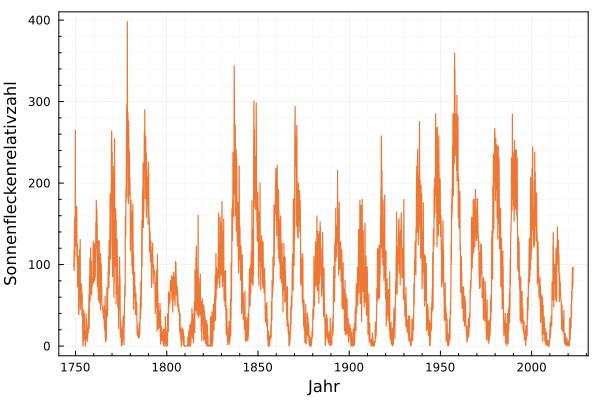
\includegraphics{./sonnenflecken_files/figure-pdf/cell-2-output-1.svg}

}

\end{figure}

Wir versuchen nun, die offensichtlich vorhandene Periodizität zu
berechnen und nutzen dafür die Schnelle Fourietransformation
\texttt{FFT}.

\begin{Shaded}
\begin{Highlighting}[]
\ImportTok{using} \BuiltInTok{FFTW}
\ImportTok{using} \BuiltInTok{Statistics}
\NormalTok{S }\OperatorTok{=} \FunctionTok{fft}\NormalTok{(SN }\OperatorTok{.{-}} \FunctionTok{mean}\NormalTok{(SN))}
\FunctionTok{popfirst!}\NormalTok{(S)}
\FunctionTok{plot}\NormalTok{(}\FunctionTok{abs}\NormalTok{.(S), label}\OperatorTok{=}\StringTok{""}\NormalTok{)}
\FunctionTok{ylabel!}\NormalTok{(}\StringTok{"Amplitudenspektrum"}\NormalTok{)}
\end{Highlighting}
\end{Shaded}

\begin{figure}[H]

{\centering 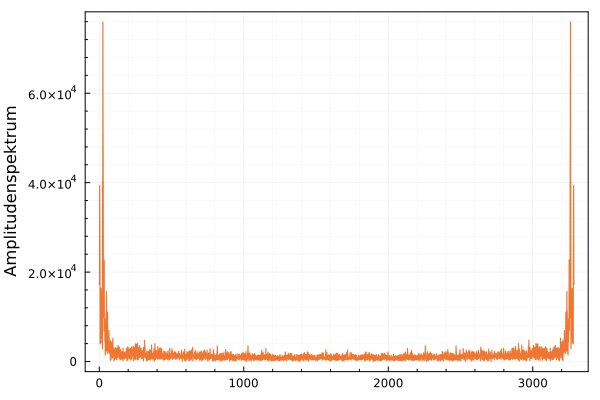
\includegraphics{./sonnenflecken_files/figure-pdf/cell-3-output-1.svg}

}

\end{figure}

\begin{Shaded}
\begin{Highlighting}[]
\NormalTok{n }\OperatorTok{=} \FunctionTok{length}\NormalTok{(S)}
\NormalTok{up }\OperatorTok{=} \FunctionTok{Int}\NormalTok{(}\FunctionTok{floor}\NormalTok{(n}\OperatorTok{/}\FloatTok{2}\NormalTok{))}
\NormalTok{power }\OperatorTok{=} \FunctionTok{abs}\NormalTok{.(S[}\FloatTok{1}\OperatorTok{:}\NormalTok{up, }\OperatorTok{:}\NormalTok{])}\OperatorTok{.\^{}}\FloatTok{2}
\NormalTok{samplinginterval }\OperatorTok{=} \FloatTok{1.0} \OperatorTok{/} \FloatTok{12.0}
\NormalTok{nyquist }\OperatorTok{=} \FloatTok{1} \OperatorTok{/}\NormalTok{ (}\FloatTok{2} \OperatorTok{*}\NormalTok{ samplinginterval)}
\NormalTok{freq }\OperatorTok{=}\NormalTok{ [}\FloatTok{1}\OperatorTok{:}\NormalTok{up}\OperatorTok{...}\NormalTok{] }\OperatorTok{./}\NormalTok{ (n }\OperatorTok{/} \FloatTok{2}\NormalTok{) }\OperatorTok{*}\NormalTok{ nyquist}
\FunctionTok{plot}\NormalTok{(freq, power)}
\FunctionTok{xlabel!}\NormalTok{(}\StringTok{"Frequenz in 1/a"}\NormalTok{)}
\FunctionTok{ylabel!}\NormalTok{(}\StringTok{"Powerspektrum"}\NormalTok{)}
\end{Highlighting}
\end{Shaded}

\begin{figure}[H]

{\centering 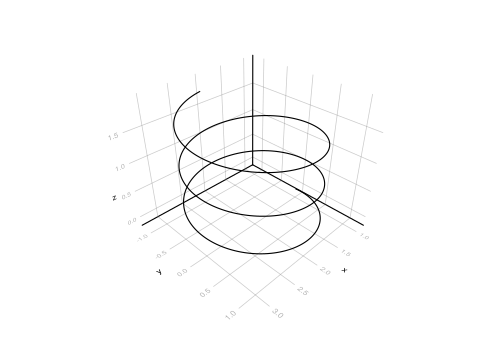
\includegraphics{./sonnenflecken_files/figure-pdf/cell-4-output-1.svg}

}

\end{figure}

\begin{Shaded}
\begin{Highlighting}[]
\NormalTok{period }\OperatorTok{=} \FloatTok{1} \OperatorTok{./}\NormalTok{ freq}
\NormalTok{i }\OperatorTok{=} \FunctionTok{argmax}\NormalTok{(power)}

\FunctionTok{plot}\NormalTok{(period, power, xscale}\OperatorTok{=:}\NormalTok{log10, label}\OperatorTok{=}\StringTok{""}\NormalTok{)}
\FunctionTok{scatter!}\NormalTok{([period[i]], [power[i]], m}\OperatorTok{=:}\NormalTok{o, label}\OperatorTok{=}\StringTok{""}\NormalTok{)}
\FunctionTok{xlabel!}\NormalTok{(}\StringTok{"Periodendauer in a"}\NormalTok{)}
\FunctionTok{ylabel!}\NormalTok{(}\StringTok{"Powerspektrum"}\NormalTok{)}
\FunctionTok{title!}\NormalTok{(}\StringTok{"Sonnenfleckenzyklus: }\SpecialCharTok{$}\NormalTok{(}\FunctionTok{round}\NormalTok{(period[i], digits}\OperatorTok{=}\FloatTok{2}\NormalTok{))}\StringTok{ a"}\NormalTok{)}
\end{Highlighting}
\end{Shaded}

\begin{figure}[H]

{\centering 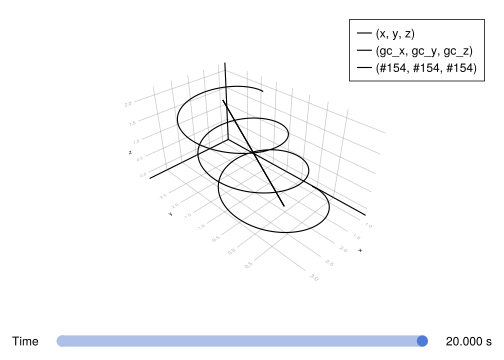
\includegraphics{./sonnenflecken_files/figure-pdf/cell-5-output-1.svg}

}

\end{figure}

\part{Plasmen und ihre Magnetfelder}

\hypertarget{plasmen}{%
\chapter{Plasmen}\label{plasmen}}

Der Begriff des Plasmas (von altgriechisch πλάσμα plásma) stammt aus dem
Griechischen und bedeutet \emph{das Gebildete, Geformte}.

Wir benutzen die folgende Definition:

\begin{tcolorbox}[enhanced jigsaw, colframe=quarto-callout-important-color-frame, colback=white, arc=.35mm, breakable, coltitle=black, titlerule=0mm, toprule=.15mm, colbacktitle=quarto-callout-important-color!10!white, bottomtitle=1mm, toptitle=1mm, rightrule=.15mm, opacitybacktitle=0.6, leftrule=.75mm, title=\textcolor{quarto-callout-important-color}{\faExclamation}\hspace{0.5em}{Wichtig}, bottomrule=.15mm, left=2mm, opacityback=0]

Ein Plasma ist ein quasineutrales Gas geladener und neutraler Teilchen
mit kollektivem Verhalten.

\end{tcolorbox}

Bewegen sich die geladenen Teilchen in einem Plasma, können sie lokale
Änderungen der Ladungsträgerdichte hervorrufen. Die Folge sind
elektrische Felder. Die Bewegung geladener Teilchen erzeugt elektrische
Ströme, die wiederum von Magnetfeldern begleitet werden. Diese
Feldeffekte beeinflussen die Bewegung geladener Teilchen in großen
Abständen.

Bewegungsmuster der Teilchen hängen nicht nur von lokalen Bedingungen,
sondern auch vom Zustand des Plasmas in entfernten Bereichen ab. Über
große Entfernungen wirksame elektromagnetische Kräfte führen dazu, dass
die Teilchen im Plasma simultan mit anderen interagieren.

Außerdem muss man unterscheiden zwischen Ladung-Ladung- und
Ladung-Neutralgas-Wechselwirkungen.

Die wichtigsten Phänomene im Zusammenhang mit dem kollektivem Verhalten
von Plasmen sind die Debye-Abschirmung sowie die Plasmafrequenz.

\hypertarget{typische-plasmen}{%
\section{Typische Plasmen}\label{typische-plasmen}}

Folgende Tabelle Tabelle~\ref{tbl-typen} gibt einen Überblick über
verschieden Plasmatypen und ihre Eigenschaften (Gibbon (2016)).

\hypertarget{tbl-typen}{}
\begin{longtable}[]{@{}lll@{}}
\caption{\label{tbl-typen}Plasmatypen}\tabularnewline
\toprule()
Typ & Elektronendichte (cm\(^{-3}\)) & Temperatur (eV) \\
\midrule()
\endfirsthead
\toprule()
Typ & Elektronendichte (cm\(^{-3}\)) & Temperatur (eV) \\
\midrule()
\endhead
Sterne & \(10^{26}\) & 2000 \\
Trägheitsfusion & \(10^{25}\) & 3000 \\
Magnetische Fusion & \(10^{15}\) & 1000 \\
Laser-generiert & \(10^{18}\) - \(10^{24}\) & 100-1000 \\
Entladung & \(10^{12}\) & 1-10 \\
Ionosphäre & \(10^{6}\) & 0.1 \\
Interstellarer Raum & 1 & 0.01 \\
\bottomrule()
\end{longtable}

(1 eV = 11600 K)

\begin{figure}

{\centering 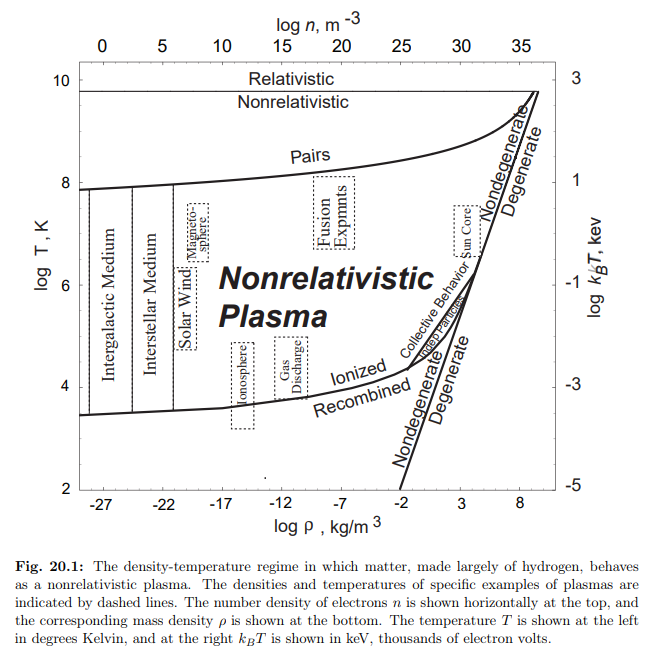
\includegraphics{./images/paste-B4955853.png}

}

\caption{\label{fig-typical-plasma}Dichte-Temperatur-Regime für typische
Plasmen (aus Thorne \& Blandford (2017))}

\end{figure}

\hypertarget{debye-luxe4nge}{%
\section{Debye-Länge}\label{debye-luxe4nge}}

Eine wichtige Eigenschaft von Plasmen ist ihre Fähigkeit, elektrische
Potentiale abzuschirmen.

Debye \& Hückel (1923a) und Debye \& Hückel (1923b) vermitteln
grundlegende Theorien zu den Wechselwirkungen von Ionen in Elektrolyten.
Diese Erkenntnisse lassen sich auf Plasmen übertragen.

\begin{figure}

{\centering 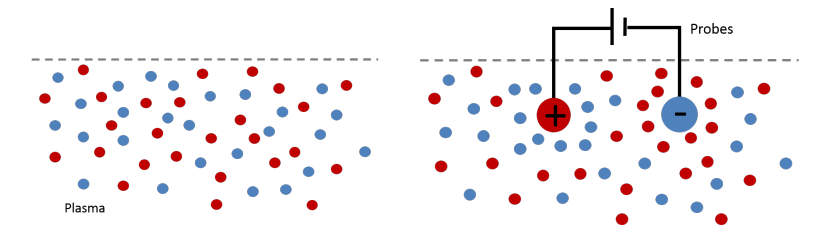
\includegraphics[width=5.83333in,height=\textheight]{./images/paste-718770F4.png}

}

\caption{\label{fig-elektrolyt}Debye-Abschirmung von geladenen Kugeln in
einem Plasma (aus Gibbon (2016))}

\end{figure}

\hypertarget{herleitung}{%
\subsection{Herleitung}\label{herleitung}}

Jedes geladene Teilchen innerhalb eines Plasmas zieht andere Teilchen
mit entgegengesetzter Ladung an und stößt Teilchen mit der gleichen
Ladung ab, wodurch in der unmittelbaren Umgebung des Teilchens eine
Wolke aus überwiegend entgegengesetzten Ladungen entsteht.

Diese Wolke schirmt die eigene Ladung des Teilchens von der Außenwelt
ab, d.~h. sie bewirkt, dass das Coulomb-Feld des Teilchens bei großen
Entfernungen exponentiell abnimmt, anstatt mit \(1/r^2\).

Diese Debye-Abschirmung der Ladung eines Teilchens kann wie folgt
demonstriert und quantifiziert werden (Thorne \& Blandford (2017)):

Man betrachte eine einzelne Testladung \(Q\) im Ursprung, die von einem
Plasma aus Protonen und Elektronen umgeben ist. Wir definieren mit
\(n_p(r)\) und \(n_e(r)\) die mittleren Dichten für Elektronen und
Protonen als glatte Funktionen des Abstandes \(r\) von der Testladung,
und mit \(\bar n\) die mittleren Dichten von Elektronen und Protonen.
Dann ist das elektrostatische Potential \(\Phi(r)\) außerhalb des
Teilchens Lösung der Poisson-Gleichung

\begin{equation}\protect\hypertarget{eq-poisson}{}{
-\nabla^2 \Phi = \frac{n_p - n_e}{\epsilon_0} e + \frac{Q}{\epsilon_0} \delta(r)
}\label{eq-poisson}\end{equation}

Wir bezeichnen die Ladung eines Protons mit \(+e\) und die Ladung des
Elektrons mit \(-e\).

Ein Proton besitzt in der Entfernung \(r\) von der Testladung das
elektrostatische Potential \(e \Phi(r)\).

Die mittlere Ladungsträgerdichte ändert sich entsprechend zu

\[
n_p(r) = \bar n \, e^{-\dfrac{e \Phi(r)}{kT}} \approx \bar n \left(1 - \frac{e \Phi}{k T} \right)
\]

bzw.

\[
n_e(r) = \bar n \, e^{+\dfrac{e \Phi(r)}{kT}} \approx \bar n \left(1 + \frac{e \Phi}{k T} \right).
\]

Damit wird Gleichung~\ref{eq-poisson} eine \emph{nichtlineare
Differentialgleichung} in \(\Phi\), weil \(n_p\) und \(n_e\) Funktionen
von \(\Phi\) sind.

Wir können aber wegen \(e\Phi \ll kT\) die Exponentialfunktion in eine
Taylorreihe entwickelt und Terme höherer Ordnung vernachlässigen.

Einsetzen in Gleichung~\ref{eq-poisson} liefert nach Linearisierung

\[
-\nabla^2 \Phi + \frac{2 \bar n e^2}{\epsilon_0 k T} \Phi = \frac{Q}{\epsilon_0}\delta(r).
\]

Die kugelsymmetrische (nur von \(r\) abhängige) Lösung ist

\[
\Phi(r) = \frac{Q}{4 \pi \epsilon_0 r} \, e^{-\sqrt{\dfrac{2r^2}{\lambda_D^2}}}
\]

und besitzt die Form eines Coulomb-Potentials mit exponentiellem Abfall.
Die charakteristische Skalenlänge dieses Abfalls ist der
\emph{Debye-Radius}

\[
\lambda_D = \sqrt{ \frac{\epsilon_0 k T}{\bar n e^2}}
\]

und ist ein Maß für die Größe der Debye-Abschirmung. Der Debye-Radius
hängt gleichermaßen von der Temperatur als auch von der Teilchendichte
des Plasmas ab. In einem idealen Plasmsa befinden sich viele Teilchen
innerhalb einer Kugel vom Radius \(\lambda_D\). Die Anzahl ist

\[
N_D = n_e \frac{4 \pi}{3} \lambda_D^3 \gg 1.
\]

\begin{figure}

{\centering 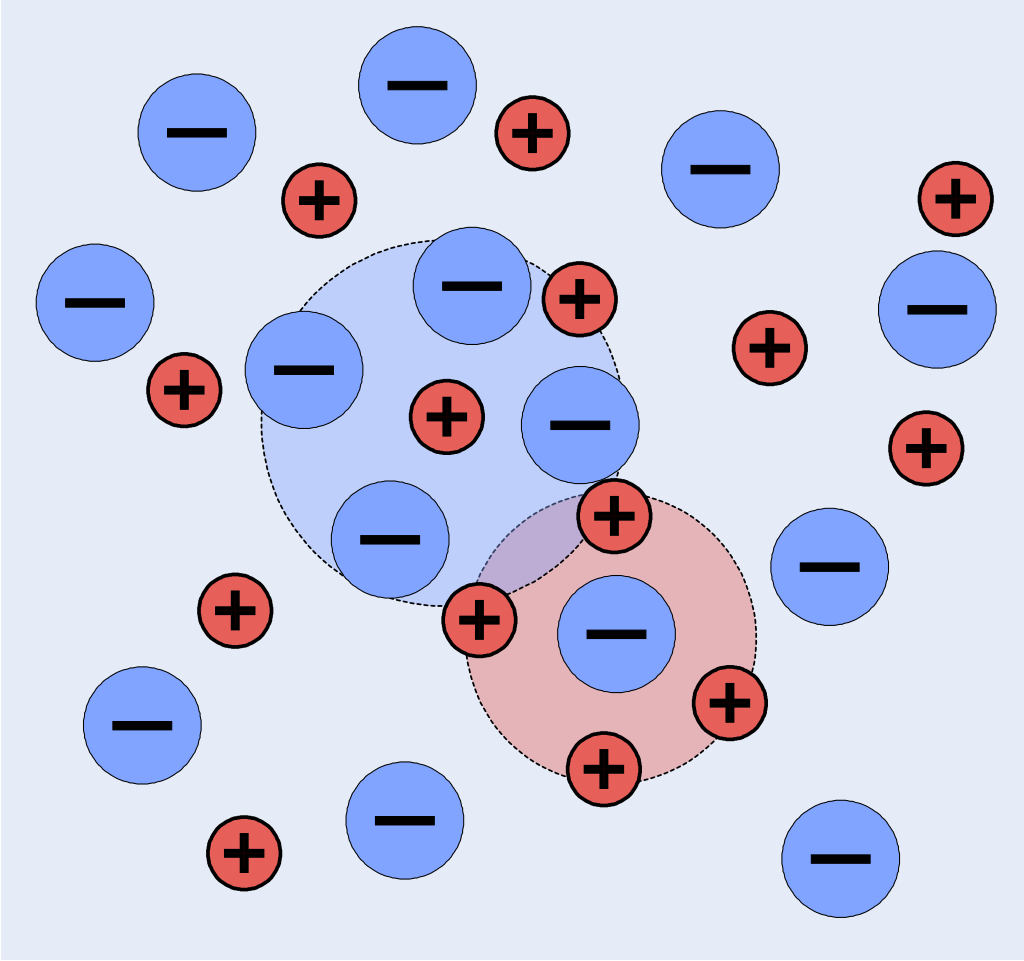
\includegraphics[width=2.1875in,height=\textheight]{./images/paste-D4D1A82B.png}

}

\caption{\label{fig-ionenverteilung}Ionenverteilung in einer Lösung (aus
Wikipedia: Debye-Länge)}

\end{figure}

Wird eine Störung (z.B. eine Überschussladung) in ein Plasma
eingebracht, so reicht die Wirkung dieser Störung nur bis zu einer
Entfernung der Größenordnung \(\lambda_D\). Nur innerhalb dieses
Abstandes weicht die lokale Ladungsträgerdichte signifikant von der
makroskopischen elektrischen Neutralität ab
(Abbildung~\ref{fig-ionenverteilung}).

\hypertarget{beispiel}{%
\subsubsection{Beispiel}\label{beispiel}}

Im Allgemeinen ist \(\lambda_D\) sehr klein. In der Ionosphäre ist
\(n_e = 10^{12}\) m\(^{-3}\) und \(T=10^3\) K. Damit ist
\(\lambda_D = 10^{-3}\) m.

\begin{figure}

{\centering 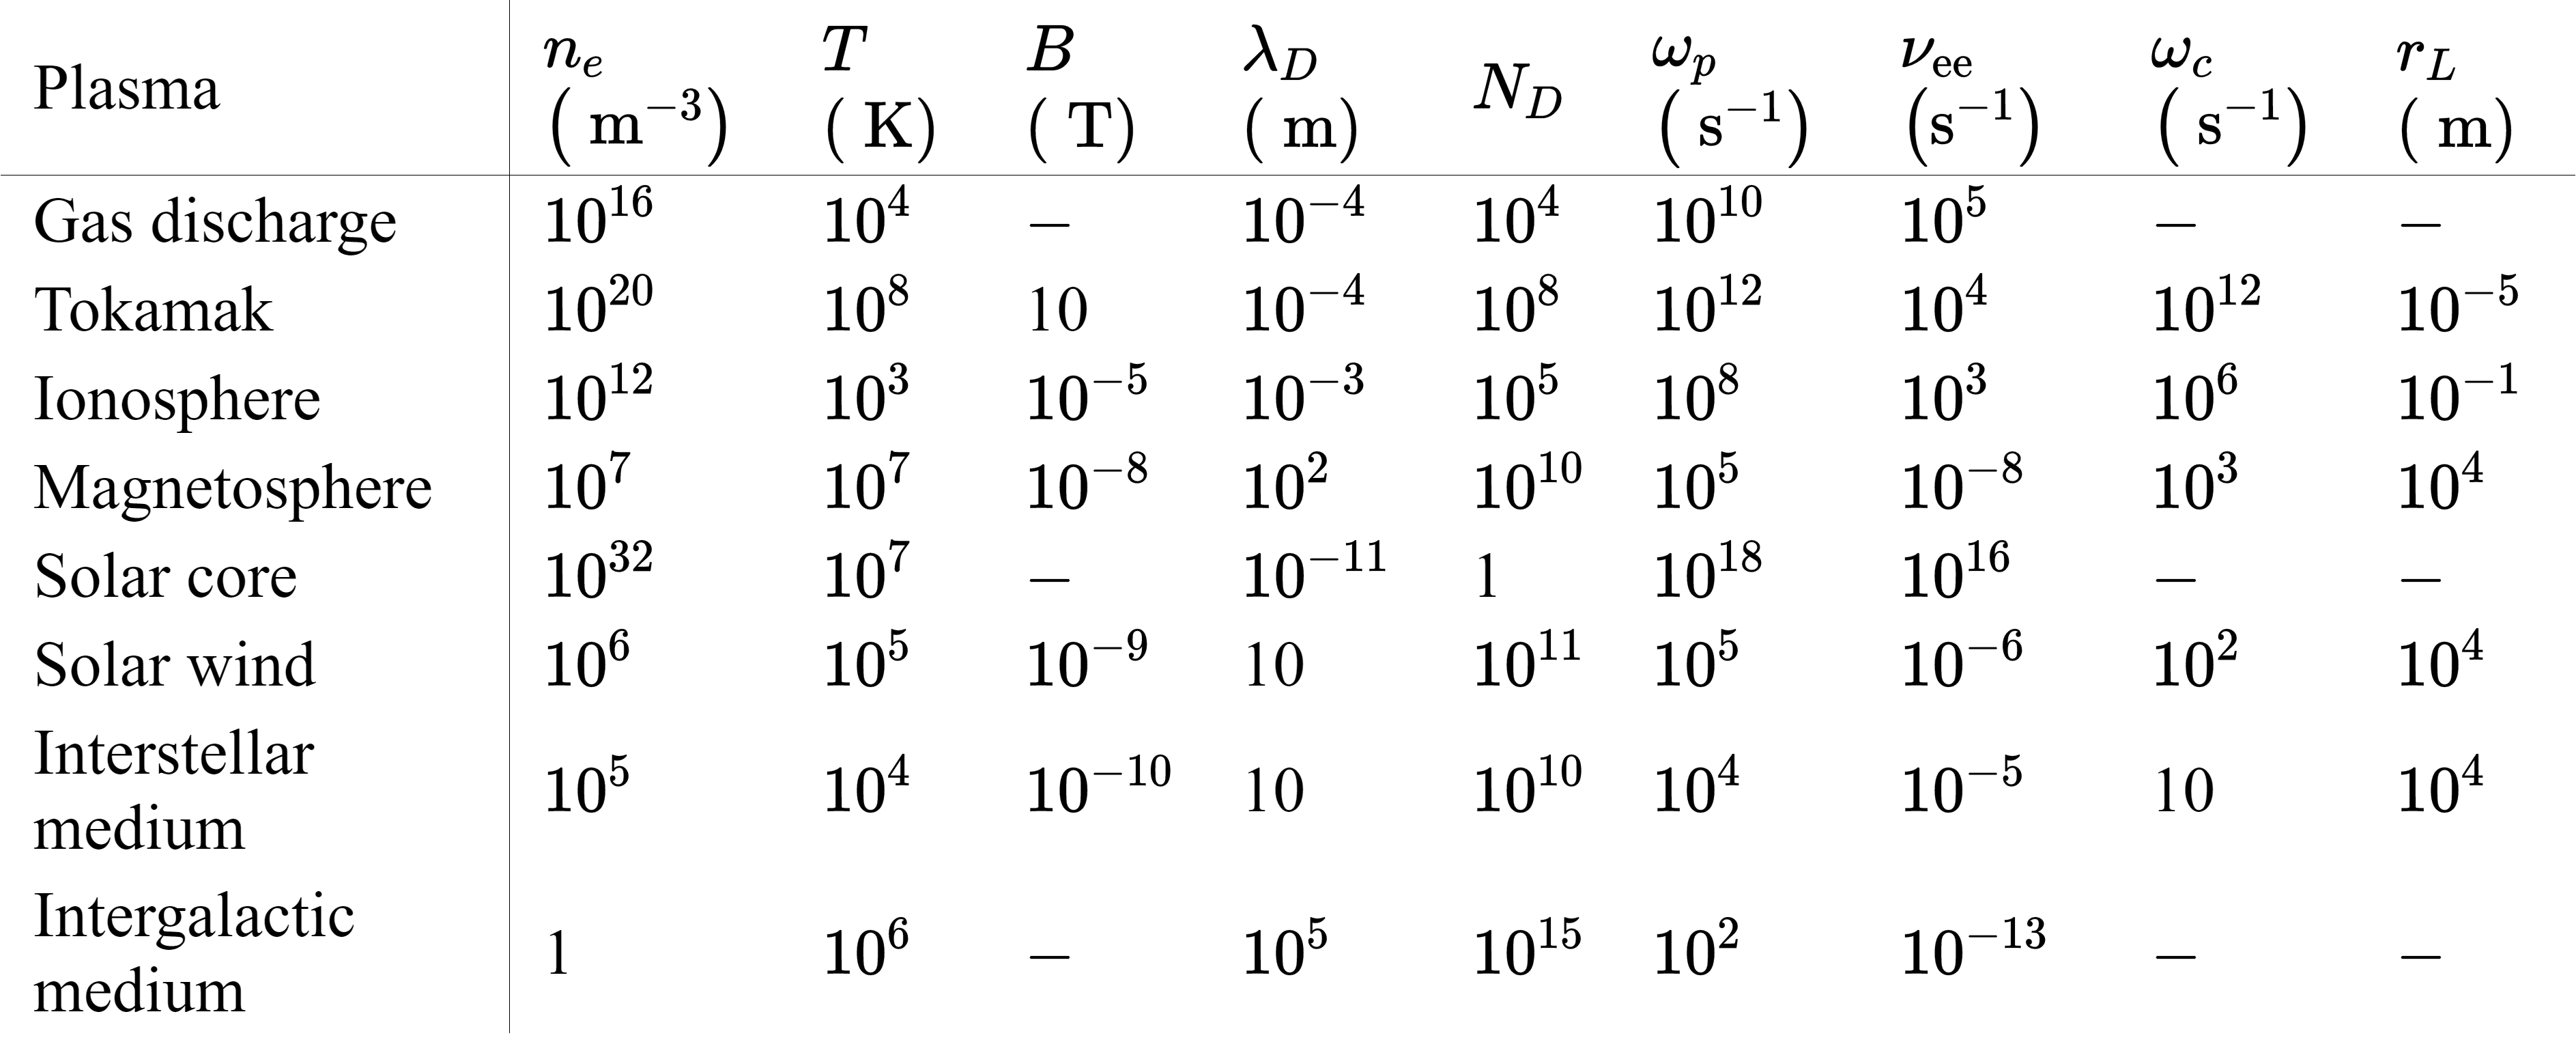
\includegraphics{./images/paste-2A0EC69D.png}

}

\caption{\label{fig-tabelle201}Typische Plasmaparameter (aus Thorne \&
Blandford (2017))}

\end{figure}

Die Tabelle in Abbildung~\ref{fig-tabelle201} gibt für typische Plasmen
die folgenden charakteristischen Größen an:

\begin{itemize}
\tightlist
\item
  Teilchendichte der Elektronen \(n_e\)
\item
  Temperatur T
\item
  Magnetfeld \(B\)
\item
  Debye-Länge \(\lambda_D\)
\item
  Debye-Zahl \(N_D\)
\item
  Plasmafrequenz \(\omega_p\)
\item
  \(\nu_{ee}\)
\item
  Larmor-Kreisfrequenz \(\omega_c\)
\item
  Larmor-Radius \(r_L\).
\end{itemize}

\hypertarget{plasmaschwingungen-und-plasmafrequenz}{%
\section{Plasmaschwingungen und
Plasmafrequenz}\label{plasmaschwingungen-und-plasmafrequenz}}

Das wichtigste dynamische Phänomen in Plasmen ist die
Schwingungsbewegung von Protonen und Elektronen relativ zueinander.

Wird ein Plasma plötzlich aus seinem Gleichgewichtszustand gebracht,
verursachen die internen Raumladungsfelder kollektive
Partikelbewegungen, welche anstreben, die ursprüngliche
Ladungsneutralität wiederherzustellen.

Diese kollektiven Schwingungsmuster laufen mit einer bestimmten
\emph{Plasma-Frequenz} ab. Wegen der hohen Frequenz tragen die
Elektroden aufgrund ihrer im Vergleich zu Protonen geringeren
Massenträgheit maßgeblich zur Plasmaschwingung bei. Elektronen schwingen
kollektiv um die schweren Ionen, wobei die Rückstellkräfte durch die
Ion-Elektron-Coulomb-Kräfte verursacht werden. Die Periodendauer dieser
Bewegung ist eine typische Zeitskala.

\begin{figure}

{\centering 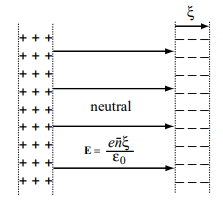
\includegraphics{./images/paste-1FB78BDE.png}

}

\caption{\label{fig-osz}Schematische Darstellung der Verschiebung von
Elektronen relativ zu Protonen während einer Plasmaschwingung (aus
Thorne \& Blandford (2017))}

\end{figure}

\hypertarget{herleitung-1}{%
\subsection{Herleitung}\label{herleitung-1}}

Wir platzieren das Plasma gemäß Abb. Abbildung~\ref{fig-osz} entlang
einer unendlich ausgedehnten Ebene in \(x=0\) und nehmen an, dass alle
Protonen ortsfest bleiben. Die Elektronen werden relativ zu den Protonen
um den Betrag \(\xi_0\) nach rechts in \(x\)-Richtung verschoben. Wir
beobachten die Flächenüberschussladungsdichten \(-e \bar n \xi_0\) am
rechten Ende des Plasmas, sowie \(+e \bar n \xi_0\) am linken Ende des
Plasmas. Das resultierende elektrische Feld im Innern des Plasmas zum
Zeitpunkt \(t=0\) ist \(\mathbf E = (E, 0, 0)^\top\), also

\[
E = \frac{e \bar n \xi_0}{\epsilon_0}.
\]

Dieses Feld übt eine Coulomb-Kraft auf die Protonen und Elektronen aus.
Die Bewegungsgleichung für die Veschiebung lautet

\[
\ddot \xi = - \frac{e}{m_e} E = - \frac{e^2 \bar n}{\epsilon_0 m_e} \xi.
\]

Dies ist eine \emph{harmonische Schwingungsdifferentialgleichung}. Wir
haben wegen des Masseverhältnisses von Elektronen zu Protonen
\(m_e/m_p = 1 / 1836\) die Kraftwirkung auf die Protonen vernachlässigt.

Mit der oben angegebene Anfangsbedingung für \(t=0\) schwingen die
Elektronen harmonisch mit den Ortskoordinaten

\[
\xi(t) = \xi_0 \cos(\omega_p t),
\]

wobei die Plasmafrequenz

\[
\omega_p = \sqrt{ \frac{\bar n e^2}{\epsilon_0 m_e} }
\]

nur von der Plasmadichte \(\bar n\) aber \emph{nicht} von der Temperatur
\(T\) oder der magnetischen Feldstärke abhängt.

Die thermische Geschwindigkeit der Elektronen ist definiert durch

\[
v_e = \sqrt{ \frac{k T}{m_e} },
\]

somit ist

\[
\omega_p = \frac{v_e}{\lambda_D}.
\]

Mit anderen Worten: Thermische Elektronen legen innerhalb einer
Plasmaschwingungsperiode etwa eine Debye-Länge zurück.

\hypertarget{newtonsche-bewegungsgleichung}{%
\chapter{Newtonsche
Bewegungsgleichung}\label{newtonsche-bewegungsgleichung}}

Die Bewegung geladener Teilchen in einem stark verdünnten Plasma lässt
sich bei Vernachlässigung von Stößen durch eine Einzelteilchentheorie
gut annähern.

Die Änderung des Bewegungszustandes eines Teilchen wird durch die
\emph{Newtonsche Bewegungsgleichung} formuliert. Die Newtonsche Mechanik
beschreibt die klassische Teilchenbewegung als eine \emph{Bahn} durch
den Euklidischen Raum und die Zeit \(t\). Zum Zeitpunkt \(t\) befindet
sich das Teilchen am Ort \(\mathbf r(t)\). Die Funktion \(\mathbf r(t)\)
beschreibt die Bahn des Teilchens im Raum. Die Teilchengeschwindigkeit
\(\mathbf v(t)\) ist die Zeitableitung der Position. Der Impuls
\(\mathbf p(t)\) ist das Produkt aus Masse \(m\) und Geschwindigkeit
\(\mathbf v(t)\). Die Zeitableitung der Geschwindigkeit ist die
Beschleunigung \(\mathbf a(t)\).

Newtons zweites Grundgesetz der Mechanik \emph{lex secunda} besagt
folgendes:

\begin{quote}
Die Änderung der Bewegung ist der Einwirkung der bewegenden Kraft
proportional und geschieht nach der Richtung derjenigen geraden Linie,
nach welcher jene Kraft wirkt.
\end{quote}

Die Änderung des Bewegungszustandes kann nur unter Wirkung von Kräften
erfolgen. Werden diese Kräfte z.B. durch ein magnetisches Feld
\(\mathbf B\), ein elektrisches Feld \(\mathbf E\) sowie ein weiteres
Kraftfeld \(\mathbf F\) erzeugt, dann nimmt die Newtonsche
Bewegungsgleichung folgende Form an:

\begin{equation}\protect\hypertarget{eq-newton}{}{
m \ddot{\mathbf r} = q (\mathbf E + \mathbf v \times \mathbf B) + \mathbf F
}\label{eq-newton}\end{equation} Diese Gleichung kann für einfache
Feldkonfigurationen trivial integriert werden. Im Falle des
geomagnetischen Feldes gibt es keine geschlossenen Lösungen, sondern nur
Näherungen. Für Teilchen mit geringer Energie, wie sie bspw. in der
Ionosphäre oder im Van-Allen-Gürtel vorliegen, steht eine Theorie zur
Approximation bereit.

Zunächst werden wir Lösungen von Gleichung~\ref{eq-newton} für
vereinfachte Bedingungen betrachten. Später werden wir sehen, dass im
Allgemeinen von den Teilchen eine schnelle Kreisbewegung ausgeführt
wird, die überlagert wird durch die Bewegung durch Magnetfelder und
elektrische Felder.

Bei Anwesenheit eines Magnetfeldes bewegen sich geladene Teilchen in
Schraubenlinien entlang der Feldlinien. Die Bewegungsgleichung für ein
mit der Geschwindigkeit \(\mathbf v\) bewegtes Teilchen der Masse \(m\)
und Ladung \(q\) im Magnetfeld \(\mathbf B\) lautet \[
m \frac{d \mathbf v}{d t} = q \mathbf v \times \mathbf B
\]

Wir betrachten zunächst den Fall eines homogenen Magnetfeldes und setzen
\[
\mathbf B = const, \quad \mathbf E = 0, \quad \mathbf F = 0
\] Die Geschwindigkeit \(\mathbf v\) zerlegen wir vektoriell in eine
Komponente parallel und eine Komponente senkrecht zum magnetischen Feld.
\[
\mathbf v = \mathbf v_\| + \mathbf v_\perp
\] Gilt \(\mathbf v_\| = const\), dann ist \(m \dot{\mathbf v}_\| = 0\)
und \[
m \dot{\mathbf v}_\perp = q \mathbf v_\perp \times \mathbf B.
\]

\hypertarget{energieerhaltung}{%
\section{Energieerhaltung}\label{energieerhaltung}}

An dieser Stelle klären wir, ob die kinetische Energie des Teilchens
eine Erhaltungsgröße ist. Da \(\mathbf v_\| = const\), betrachten wir
die Änderung der kinetischen Energie \[
\frac{d E_{kin}}{d t} = \frac{d}{dt} \left( \frac{1}{2} m |\mathbf v_\perp|^2  \right) =
\mathbf v_\perp \cdot (m \dot{\mathbf v}_\perp) = q \mathbf v_\perp \cdot \left( \mathbf v_\perp \times \mathbf B \right) \overset{!}{=} 0.
\] Damit ist gezeigt, dass die kinetische Energie eines Teilchens im
Magnetfeld eine Erhaltungsgröße ist. Ein statisches Magnetfeld ändert
also weder \(\mathbf v\) noch die kinetische Energie. Dies ist eine sehr
wichtige Erkenntnis mit weitreichenden Konsequenzen für den Fall, dass
das Magnetfeld zeitlich variabel oder inhomogen ist.

\hypertarget{flugbahn}{%
\section{Flugbahn}\label{flugbahn}}

Bewegt sich das Teilchen in einer Ebene senkrecht zu \(\mathbf B\), dann
gilt \[
\mathbf v _\| \times \mathbf B = \mathbf 0
\] und \[
\mathbf v_\perp \times \mathbf B \perp \mathbf B.
\] Es gilt wegen \(\mathbf v = \mathbf \omega \times \mathbf r\)
(Bahngeschwindigkeit gleich Kreuzprodukt aus Winkelgeschwindigkeit und
Ortsvektor) \begin{equation}\protect\hypertarget{eq-gyration}{}{
\dot{\mathbf v}_\perp = \frac{q}{m} \left( \mathbf v_\perp \times \mathbf B \right) = \boldsymbol \omega_g \times \mathbf v_\perp
}\label{eq-gyration}\end{equation} Die Größe \(\mathbf \omega_g\) ist
die vektorielle Winkelgeschwindigkeit der Kreisbewegung. Es folgt \[
\boldsymbol \omega_g = - \frac{q}{m} \mathbf B = 
\frac{|q|}{m} B \, \widehat{\boldsymbol \omega}_g =
\omega_g \widehat{\boldsymbol \omega}_g
\] Der Betrag der Winkelgeschwindigkeit wird als Zyklotronfrequenz (oder
Larmorfrequenz) bezeichnet. \(\widehat{\mathbf \omega}_g\) ist der
Einheitsvektor der Winkelgeschwindigkeit. Mit der Rechte-Hand-Regel
ergibt sich die Bewegungsrichtung. Die Richtung der Kreisbewegung hängt
vom Vorzeichen der Ladung des Teilchen ab. Es gilt \[
q < 0: \qquad \widehat{\boldsymbol \omega}_g \| \mathbf B \qquad \text{parallel}
\] \[
q > 0: \qquad -\widehat{\boldsymbol \omega}_g \| \mathbf B \qquad \text{antiparallel}
\] Integrieren wir Gleichung~\ref{eq-gyration} zeitlich, erkennen wir
den Zusammenhang zwischen Bahngeschwindigkeit und Teilchenposition. Es
gilt \[
\mathbf v_\perp = \boldsymbol \omega_g \times \mathbf r_g
\] Mit \(\mathbf r_g\) bezeichnen wir die Teilchenposition. Sie
beschreibt eine Kreisbahn mit Radius \(r_g\) um den
Gyrationsmittelpunkt, der auch als \emph{Führungszentrum} bezeichnet
wird.

\hypertarget{beispiel-1}{%
\subsection{Beispiel}\label{beispiel-1}}

Wir berechnen die Zyklotronfrequenz und den Gyratonsradius für ein
Elektron. Die Elektronenmasse ist \[
m_e = 9.109 \times 10^{-31} ~\text{kg},
\] seine Ladung entspricht der Elementarladung \[
|q| = e = 1.602 \times 10^{-19} ~ \text{C}.
\] Wird \(\mathbf B\) in Tesla angegeben, gilt für die Zyklotronfrequenz
des Elektrons die Gleichung \[
\omega_c^e = \frac{e B}{m_e} = 1.76 \times 10^{11} \, B \text{ in rad}\cdot s^{-1}
\] Da Protonen eine um den Faktor 1890 größere Masse als Elektronen
besitzen, ist ihre Zyklotronfrequenz niedriger: \[
\omega_c^p = \frac{e B}{m_p} = 9.58 \times 10^{7} \, B \text{ in rad}\cdot s^{-1}
\] Der Gyrationsradius ist \[
r_g = \frac{v_\perp}{\omega_g} = \frac{m v_\perp}{|q| B}.
\]

\hypertarget{zusammenfassung}{%
\section{Zusammenfassung}\label{zusammenfassung}}

\begin{figure}

{\centering 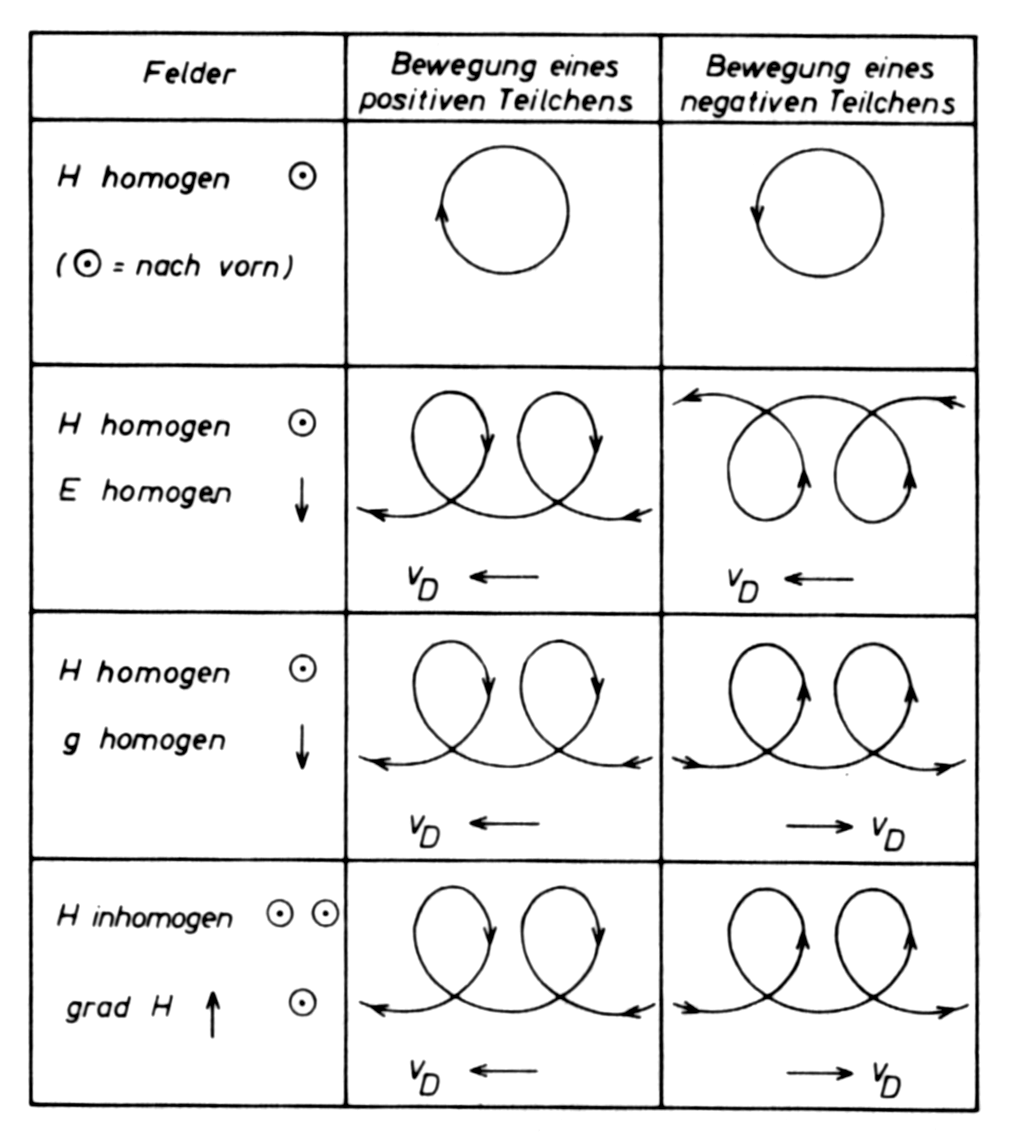
\includegraphics{./images/gyration.png}

}

\caption{Bewegung geladener Teilchen im Magnetfeld (aus (Kertz 1971)).}

\end{figure}

\hypertarget{proton-und-elektron}{%
\chapter{Proton und Elektron}\label{proton-und-elektron}}

\begin{Shaded}
\begin{Highlighting}[]
\ImportTok{using} \BuiltInTok{TestParticle}
\ImportTok{using} \BuiltInTok{Meshes}
\ImportTok{using} \BuiltInTok{OrdinaryDiffEq}
\ImportTok{using} \BuiltInTok{Plots}
\ImportTok{using} \BuiltInTok{Markdown}
\FunctionTok{theme}\NormalTok{(}\OperatorTok{:}\NormalTok{vibrant)}
\FunctionTok{default}\NormalTok{(widen}\OperatorTok{=}\ConstantTok{false}\NormalTok{)}

\KeywordTok{function} \FunctionTok{circle}\NormalTok{(radius, center, N)}
\NormalTok{    θ }\OperatorTok{=} \FunctionTok{range}\NormalTok{(}\FloatTok{0}\NormalTok{, }\FloatTok{2}\NormalTok{π, N)}
\NormalTok{    center[}\FloatTok{1}\NormalTok{] }\OperatorTok{.+}\NormalTok{ radius }\OperatorTok{*} \FunctionTok{cos}\NormalTok{.(θ), center[}\FloatTok{2}\NormalTok{] }\OperatorTok{.+}\NormalTok{ radius }\OperatorTok{*} \FunctionTok{sin}\NormalTok{.(θ)}
\KeywordTok{end}
\end{Highlighting}
\end{Shaded}

\begin{verbatim}
circle (generic function with 1 method)
\end{verbatim}

Wir betrachten den Fall, dass das Teilchen mit der Geschwindigkeit
\(\mathbf v = \mathbf v_\perp\) in ein Magnetfeld \(\mathbf B\) und
elektrisches Feld \(\mathbf E\) eingebracht wird.

Die Bewegungsgleichung lautet \[
\dot{\mathbf v}_\perp = \frac{q}{m} \left( \mathbf E +  \mathbf v_\perp \times \mathbf B \right)
\]

Vereinfachend nehmen wir zunächst an, dass \(\mathbf E = \mathbf 0\).
Weiterhin sei \(\mathbf B = (0, 0, B)^\top\) homogen.

Aus der Lösung berechnen wir die Kreisfrequenz der Gyrationsbewegung \[
\omega_g = \frac{|q| B}{m}
\] und den Gyrationsradius \[
r_g = \frac{m v_\perp}{|q| B}.
\]

\hypertarget{numerisches-beispiel}{%
\section{Numerisches Beispiel}\label{numerisches-beispiel}}

Wir berechnen die Gyrationsfrequenz und den Gyrationsradius für
nichtrelativistische Elektronen und Protonen. Die Ladung eines Protons
beträgt \(q = +e = +1.60217662 \times 10^{-19}\) C, seine Masse ist
\(1.673557546 \times 10^{-27}\) kg. Die Ladung eines Elektrons beträgt
\(q = -e = -1.60217662 \times 10^{-19}\) C, seine Masse ist
\(9.10938356 \times 10^{-31}\) kg.

Im Magnetfeld der Stärke \(B = 1\) nT erhalten wir für die
Gyrationsfrequenz \[
f_g = \frac{\omega_g}{2 \pi} = \frac{|q| B}{2 \pi m}
\]

\begin{Shaded}
\begin{Highlighting}[]
\NormalTok{m\_p }\OperatorTok{=}\NormalTok{ TestParticle.mᵢ}
\NormalTok{m\_e }\OperatorTok{=}\NormalTok{ TestParticle.mₑ}
\NormalTok{q\_p }\OperatorTok{=}\NormalTok{ TestParticle.qᵢ}
\NormalTok{q\_e }\OperatorTok{=}\NormalTok{ TestParticle.qₑ}
\NormalTok{B }\OperatorTok{=} \FloatTok{1.0e{-}9}
\NormalTok{v }\OperatorTok{=} \FloatTok{1.0}

\NormalTok{f\_p }\OperatorTok{=}\NormalTok{ q\_p }\OperatorTok{*}\NormalTok{ B }\OperatorTok{/}\NormalTok{ (}\FloatTok{2} \OperatorTok{*} \ConstantTok{pi} \OperatorTok{*}\NormalTok{ m\_p) }
\NormalTok{f\_e }\OperatorTok{=} \FunctionTok{abs}\NormalTok{(q\_e) }\OperatorTok{*}\NormalTok{ B }\OperatorTok{/}\NormalTok{ (}\FloatTok{2} \OperatorTok{*} \ConstantTok{pi} \OperatorTok{*}\NormalTok{ m\_e) }

\NormalTok{r\_p }\OperatorTok{=}\NormalTok{ m\_p }\OperatorTok{*}\NormalTok{ v }\OperatorTok{/} \FunctionTok{abs}\NormalTok{(q\_p) }\OperatorTok{/}\NormalTok{ B}
\NormalTok{r\_e }\OperatorTok{=}\NormalTok{ m\_e }\OperatorTok{*}\NormalTok{ v }\OperatorTok{/} \FunctionTok{abs}\NormalTok{(q\_e) }\OperatorTok{/}\NormalTok{ B}

\NormalTok{Markdown.}\FunctionTok{parse}\NormalTok{(}\StringTok{"""}
\StringTok{Die Gyrationsfrequenz für Protonen beträgt }\SpecialCharTok{$}\NormalTok{(}\FunctionTok{round}\NormalTok{(f\_p, digits}\OperatorTok{=}\FloatTok{3}\NormalTok{))}\StringTok{ Hz.}
\StringTok{Die Gyrationsfrequenz für Elektronen beträgt }\SpecialCharTok{$}\NormalTok{(}\FunctionTok{round}\NormalTok{(f\_e, digits}\OperatorTok{=}\FloatTok{3}\NormalTok{))}\StringTok{ Hz.}
\StringTok{Der Gyrationsradius für Protonen beträgt }\SpecialCharTok{$}\NormalTok{(}\FunctionTok{round}\NormalTok{(r\_p, sigdigits}\OperatorTok{=}\FloatTok{3}\NormalTok{))}\StringTok{ m.}
\StringTok{Der Gyrationsradius für Elektronen beträgt }\SpecialCharTok{$}\NormalTok{(}\FunctionTok{round}\NormalTok{(r\_e, sigdigits}\OperatorTok{=}\FloatTok{3}\NormalTok{))}\StringTok{ m.}
\StringTok{"""}\NormalTok{)}
\end{Highlighting}
\end{Shaded}

Die Gyrationsfrequenz für Protonen beträgt 0.015 Hz. Die
Gyrationsfrequenz für Elektronen beträgt 27.992 Hz. Der Gyrationsradius
für Protonen beträgt 10.4 m. Der Gyrationsradius für Elektronen beträgt
0.00569 m.

\begin{Shaded}
\begin{Highlighting}[]
\NormalTok{x }\OperatorTok{=} \FunctionTok{range}\NormalTok{(}\OperatorTok{{-}}\FloatTok{20}\NormalTok{, }\FloatTok{20}\NormalTok{, length}\OperatorTok{=}\FloatTok{41}\NormalTok{)}
\NormalTok{y }\OperatorTok{=} \FunctionTok{range}\NormalTok{(}\OperatorTok{{-}}\FloatTok{20}\NormalTok{, }\FloatTok{20}\NormalTok{, length}\OperatorTok{=}\FloatTok{41}\NormalTok{)}
\NormalTok{z }\OperatorTok{=} \FunctionTok{range}\NormalTok{(}\OperatorTok{{-}}\FloatTok{20}\NormalTok{, }\FloatTok{20}\NormalTok{, length}\OperatorTok{=}\FloatTok{41}\NormalTok{)}
\NormalTok{B }\OperatorTok{=} \FunctionTok{fill}\NormalTok{(}\FloatTok{0.0}\NormalTok{, }\FloatTok{3}\NormalTok{, }\FunctionTok{length}\NormalTok{(x), }\FunctionTok{length}\NormalTok{(y), }\FunctionTok{length}\NormalTok{(z)) }\CommentTok{\# [T]}
\NormalTok{E }\OperatorTok{=} \FunctionTok{fill}\NormalTok{(}\FloatTok{0.0}\NormalTok{, }\FloatTok{3}\NormalTok{, }\FunctionTok{length}\NormalTok{(x), }\FunctionTok{length}\NormalTok{(y), }\FunctionTok{length}\NormalTok{(z)) }\CommentTok{\# [V/m]}
\NormalTok{B[}\FloatTok{3}\NormalTok{,}\OperatorTok{:}\NormalTok{,}\OperatorTok{:}\NormalTok{,}\OperatorTok{:}\NormalTok{] }\OperatorTok{.=} \FloatTok{1e{-}9}
\CommentTok{\# E[2,:,:,:] .= 1e{-}10}
\ConstantTok{nothing}
\end{Highlighting}
\end{Shaded}

\begin{Shaded}
\begin{Highlighting}[]
\NormalTok{Δx }\OperatorTok{=}\NormalTok{ x[}\FloatTok{2}\NormalTok{] }\OperatorTok{{-}}\NormalTok{ x[}\FloatTok{1}\NormalTok{]}
\NormalTok{Δy }\OperatorTok{=}\NormalTok{ y[}\FloatTok{2}\NormalTok{] }\OperatorTok{{-}}\NormalTok{ y[}\FloatTok{1}\NormalTok{]}
\NormalTok{Δz }\OperatorTok{=}\NormalTok{ z[}\FloatTok{2}\NormalTok{] }\OperatorTok{{-}}\NormalTok{ z[}\FloatTok{1}\NormalTok{]}

\NormalTok{grid }\OperatorTok{=} \FunctionTok{CartesianGrid}\NormalTok{((}\FunctionTok{length}\NormalTok{(x)}\OperatorTok{{-}}\FloatTok{1}\NormalTok{, }\FunctionTok{length}\NormalTok{(y)}\OperatorTok{{-}}\FloatTok{1}\NormalTok{, }\FunctionTok{length}\NormalTok{(z)}\OperatorTok{{-}}\FloatTok{1}\NormalTok{),}
\NormalTok{   (x[}\FloatTok{1}\NormalTok{], y[}\FloatTok{1}\NormalTok{], z[}\FloatTok{1}\NormalTok{]),}
\NormalTok{   (Δx, Δy, Δz))}
\ConstantTok{nothing}
\end{Highlighting}
\end{Shaded}

\begin{Shaded}
\begin{Highlighting}[]
\NormalTok{isAnalytic }\OperatorTok{=} \ConstantTok{false}
\NormalTok{trajectories }\OperatorTok{=} \FloatTok{1}

\NormalTok{x0 }\OperatorTok{=}\NormalTok{ [}\OperatorTok{{-}}\FloatTok{1.0}\NormalTok{, }\FloatTok{0.0}\NormalTok{, }\FloatTok{0.0}\NormalTok{] }\CommentTok{\# initial position, [m]}
\NormalTok{u0 }\OperatorTok{=}\NormalTok{ [}\FloatTok{0.0}\NormalTok{, }\FloatTok{1.0}\NormalTok{, }\FloatTok{0.0}\NormalTok{] }\CommentTok{\# initial velocity, [m/s]}
\NormalTok{stateinit }\OperatorTok{=}\NormalTok{ [x0}\OperatorTok{...}\NormalTok{, u0}\OperatorTok{...}\NormalTok{]}

\NormalTok{param\_electron }\OperatorTok{=} \FunctionTok{prepare}\NormalTok{(grid, E, B, species}\OperatorTok{=}\NormalTok{Electron)}
\NormalTok{tspan\_electron }\OperatorTok{=}\NormalTok{ (}\FloatTok{0.0}\NormalTok{, }\FloatTok{0.1}\NormalTok{)}

\NormalTok{param\_proton }\OperatorTok{=} \FunctionTok{prepare}\NormalTok{(grid, E, B, species}\OperatorTok{=}\NormalTok{Proton)}
\NormalTok{tspan\_proton }\OperatorTok{=}\NormalTok{ (}\FloatTok{0.0}\NormalTok{, }\FloatTok{200.0}\NormalTok{)}

\NormalTok{prob\_e }\OperatorTok{=} \FunctionTok{ODEProblem}\NormalTok{(trace!, stateinit, tspan\_electron, param\_electron)}
\NormalTok{prob\_p }\OperatorTok{=} \FunctionTok{ODEProblem}\NormalTok{(trace!, stateinit, tspan\_proton, param\_proton)}
\NormalTok{sol\_e }\OperatorTok{=} \FunctionTok{solve}\NormalTok{(prob\_e, }\FunctionTok{Tsit5}\NormalTok{(); save\_idxs}\OperatorTok{=}\NormalTok{[}\FloatTok{1}\NormalTok{,}\FloatTok{2}\NormalTok{,}\FloatTok{3}\NormalTok{])}
\NormalTok{sol\_p }\OperatorTok{=} \FunctionTok{solve}\NormalTok{(prob\_p, }\FunctionTok{Tsit5}\NormalTok{(); save\_idxs}\OperatorTok{=}\NormalTok{[}\FloatTok{1}\NormalTok{,}\FloatTok{2}\NormalTok{,}\FloatTok{3}\NormalTok{]);}
\end{Highlighting}
\end{Shaded}

\begin{Shaded}
\begin{Highlighting}[]
\FunctionTok{plot}\NormalTok{(sol\_e, idxs}\OperatorTok{=}\NormalTok{(}\FloatTok{1}\NormalTok{,}\FloatTok{2}\NormalTok{), lw}\OperatorTok{=}\FloatTok{3}\NormalTok{, label}\OperatorTok{=}\StringTok{"Elektron"}\NormalTok{)}

\NormalTok{c }\OperatorTok{=} \FunctionTok{circle}\NormalTok{(r\_e ,[}\OperatorTok{{-}}\FloatTok{1.0} \OperatorTok{{-}}\NormalTok{ r\_e; }\FloatTok{0.0}\NormalTok{], }\FloatTok{32}\NormalTok{);}
\FunctionTok{plot!}\NormalTok{(c[}\FloatTok{1}\NormalTok{], c[}\FloatTok{2}\NormalTok{], label}\OperatorTok{=}\StringTok{"analytisch"}\NormalTok{, lw}\OperatorTok{=}\FloatTok{0.5}\NormalTok{, aspect\_ratio}\OperatorTok{=:}\NormalTok{equal)}
\end{Highlighting}
\end{Shaded}

\begin{figure}[H]

{\centering 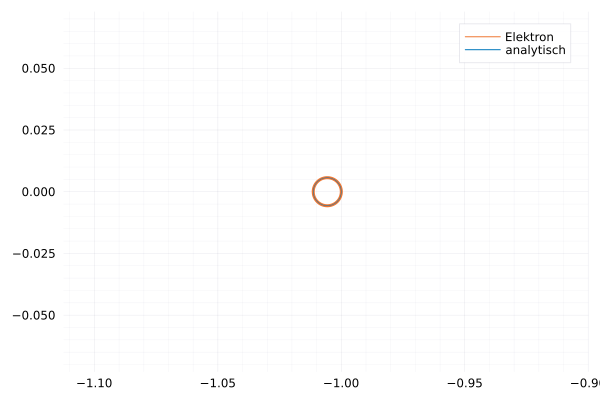
\includegraphics{./motion_homogen_files/figure-pdf/cell-7-output-1.svg}

}

\end{figure}

\begin{Shaded}
\begin{Highlighting}[]
\FunctionTok{plot}\NormalTok{(sol\_p, idxs}\OperatorTok{=}\NormalTok{(}\FloatTok{1}\NormalTok{,}\FloatTok{2}\NormalTok{), lw}\OperatorTok{=}\FloatTok{3}\NormalTok{, label}\OperatorTok{=}\StringTok{"Proton"}\NormalTok{)}

\NormalTok{c }\OperatorTok{=} \FunctionTok{circle}\NormalTok{(r\_p ,[}\OperatorTok{{-}}\FloatTok{1.0} \OperatorTok{+}\NormalTok{ r\_p; }\FloatTok{0.0}\NormalTok{], }\FloatTok{64}\NormalTok{);}
\FunctionTok{plot!}\NormalTok{(c[}\FloatTok{1}\NormalTok{], c[}\FloatTok{2}\NormalTok{], label}\OperatorTok{=}\StringTok{"analytisch"}\NormalTok{, lw}\OperatorTok{=}\FloatTok{0.5}\NormalTok{, aspect\_ratio}\OperatorTok{=:}\NormalTok{equal)}
\end{Highlighting}
\end{Shaded}

\begin{figure}[H]

{\centering 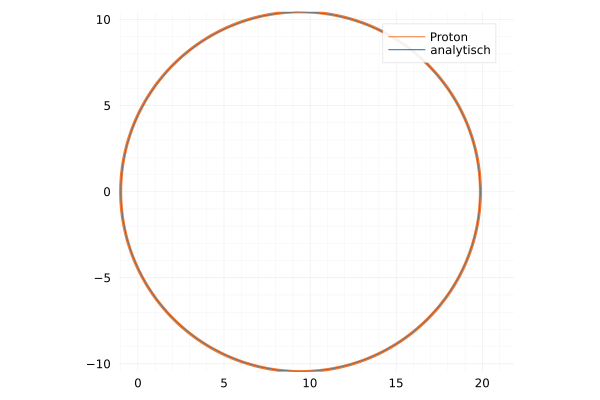
\includegraphics{./motion_homogen_files/figure-pdf/cell-8-output-1.svg}

}

\end{figure}

\hypertarget{simulation-der-teilchenbewegung-mit-julia}{%
\chapter{Simulation der Teilchenbewegung mit
Julia}\label{simulation-der-teilchenbewegung-mit-julia}}

Dieses Notebook demonstriert die numerische Simulation der
Teilchenbewegung.

Wir nutzen einen ODE-Löser des Julia-Pakets \emph{OrdinaryDiffEq}.
Außerdem nutzen wir \emph{TestParticle.jl}, ein Paket zum bequemen
Berechnen der Bewegungsbahnen geladener Teilchen in Dipolfeldern.

Die Visualisierung erfolgt mit \emph{Plots.jl}.

\begin{Shaded}
\begin{Highlighting}[]
\ImportTok{using} \BuiltInTok{TestParticle}
\ImportTok{using} \BuiltInTok{TestParticle}\NormalTok{: getB\_dipole, getE\_dipole, sph2cart, Rₑ}
\ImportTok{using} \BuiltInTok{OrdinaryDiffEq}
\ImportTok{using} \BuiltInTok{Plots}
\ImportTok{using} \BuiltInTok{Statistics}
\end{Highlighting}
\end{Shaded}

\begin{Shaded}
\begin{Highlighting}[]
\KeywordTok{function} \FunctionTok{fieldline}\NormalTok{(ϕ}\OperatorTok{::}\DataTypeTok{Float64}\NormalTok{, L}\OperatorTok{::}\DataTypeTok{Float64}\NormalTok{=}\FloatTok{2.5}\NormalTok{, nP}\OperatorTok{::}\DataTypeTok{Int}\NormalTok{=}\FloatTok{100}\NormalTok{)}

\NormalTok{   xyz }\OperatorTok{=}\NormalTok{ [ }\FunctionTok{sph2cart}\NormalTok{(}\FunctionTok{L*sin}\NormalTok{(θ)}\OperatorTok{\^{}}\FloatTok{2}\NormalTok{,ϕ,θ) for θ }\KeywordTok{in} \FunctionTok{range}\NormalTok{(}\OperatorTok{{-}}\ConstantTok{π}\NormalTok{,stop}\OperatorTok{=}\ConstantTok{π}\NormalTok{,length}\OperatorTok{=}\NormalTok{nP) ]}
\NormalTok{   x }\OperatorTok{=} \FunctionTok{Vector}\DataTypeTok{\{Float64\}}\NormalTok{(}\ConstantTok{undef}\NormalTok{,}\FunctionTok{length}\NormalTok{(xyz))}
\NormalTok{   y }\OperatorTok{=} \FunctionTok{Vector}\DataTypeTok{\{Float64\}}\NormalTok{(}\ConstantTok{undef}\NormalTok{,}\FunctionTok{length}\NormalTok{(xyz))}
\NormalTok{   z }\OperatorTok{=} \FunctionTok{Vector}\DataTypeTok{\{Float64\}}\NormalTok{(}\ConstantTok{undef}\NormalTok{,}\FunctionTok{length}\NormalTok{(xyz))}

   \ControlFlowTok{for}\NormalTok{ (i, pos) }\KeywordTok{in} \FunctionTok{enumerate}\NormalTok{(xyz)}
\NormalTok{      x[i],y[i],z[i] }\OperatorTok{=}\NormalTok{ [pos}\OperatorTok{...}\NormalTok{]}
   \ControlFlowTok{end}

\NormalTok{   (x,y,z)}
\KeywordTok{end}
\end{Highlighting}
\end{Shaded}

\begin{verbatim}
fieldline (generic function with 3 methods)
\end{verbatim}

\begin{Shaded}
\begin{Highlighting}[]
\KeywordTok{function} \FunctionTok{plot\_iso3d}\NormalTok{(xs, ys, zs; lw}\OperatorTok{=}\FloatTok{3}\NormalTok{, lc}\OperatorTok{=:}\NormalTok{red, title}\OperatorTok{=}\StringTok{"Isometric 3D plot"}\NormalTok{,label}\OperatorTok{=}\ConstantTok{false}\NormalTok{, camera}\OperatorTok{=}\NormalTok{(}\FloatTok{45}\NormalTok{,}\FloatTok{30}\NormalTok{))}
    \CommentTok{\# condition data for nearly isometric 3D plot }
\NormalTok{    x12, y12, z12 }\OperatorTok{=} \FunctionTok{extrema}\NormalTok{(xs), }\FunctionTok{extrema}\NormalTok{(ys), }\FunctionTok{extrema}\NormalTok{(zs)}
\NormalTok{    d }\OperatorTok{=} \FunctionTok{maximum}\NormalTok{([}\FunctionTok{diff}\NormalTok{([x12}\OperatorTok{...}\NormalTok{]),}\FunctionTok{diff}\NormalTok{([y12}\OperatorTok{...}\NormalTok{]),}\FunctionTok{diff}\NormalTok{([z12}\OperatorTok{...}\NormalTok{])])[}\FloatTok{1}\NormalTok{] }\OperatorTok{/} \FloatTok{2}
\NormalTok{    xm, ym, zm }\OperatorTok{=} \FunctionTok{mean}\NormalTok{(x12),  }\FunctionTok{mean}\NormalTok{(y12),  }\FunctionTok{mean}\NormalTok{(z12) }

    \CommentTok{\# plot data}
\NormalTok{    p }\OperatorTok{=}\NormalTok{ Plots.}\FunctionTok{plot}\NormalTok{(; xlabel}\OperatorTok{=}\StringTok{"x"}\NormalTok{,ylabel}\OperatorTok{=}\StringTok{"y"}\NormalTok{,zlabel}\OperatorTok{=}\StringTok{"z"}\NormalTok{, aspect\_ratio}\OperatorTok{=:}\NormalTok{equal, grid}\OperatorTok{=:}\ConstantTok{true}\NormalTok{)}
\NormalTok{    Plots.}\FunctionTok{plot!}\NormalTok{(xlims}\OperatorTok{=}\NormalTok{(xm}\OperatorTok{{-}}\NormalTok{d,xm}\OperatorTok{+}\NormalTok{d), ylims}\OperatorTok{=}\NormalTok{(ym}\OperatorTok{{-}}\NormalTok{d,ym}\OperatorTok{+}\NormalTok{d), zlims}\OperatorTok{=}\NormalTok{(zm}\OperatorTok{{-}}\NormalTok{d,zm}\OperatorTok{+}\NormalTok{d))}
\NormalTok{    Plots.}\FunctionTok{plot!}\NormalTok{(;camera}\OperatorTok{=}\NormalTok{camera)    }\CommentTok{\#(azimuth,elevation) ???}
\NormalTok{    Plots.}\FunctionTok{plot!}\NormalTok{(xs, ys, zs, title}\OperatorTok{=}\NormalTok{title,lw}\OperatorTok{=}\NormalTok{lw,lc}\OperatorTok{=}\NormalTok{lc,label}\OperatorTok{=}\NormalTok{label)}
\NormalTok{    Plots.}\FunctionTok{plot!}\NormalTok{(xs, ys, }\FunctionTok{zlims}\NormalTok{(p)[}\FloatTok{1}\NormalTok{] }\OperatorTok{.+} \FloatTok{0}\OperatorTok{*}\NormalTok{zs, lw}\OperatorTok{=}\FloatTok{1}\NormalTok{, lc}\OperatorTok{=:}\NormalTok{lightgray, label}\OperatorTok{=}\ConstantTok{false}\NormalTok{)}
\NormalTok{    Plots.}\FunctionTok{plot!}\NormalTok{(xs, }\FunctionTok{ylims}\NormalTok{(p)[}\FloatTok{2}\NormalTok{]  }\OperatorTok{.+} \FloatTok{0}\OperatorTok{*}\NormalTok{ys, zs, lw}\OperatorTok{=}\FloatTok{1}\NormalTok{, lc}\OperatorTok{=:}\NormalTok{lightgray, label}\OperatorTok{=}\ConstantTok{false}\NormalTok{)}
\NormalTok{    Plots.}\FunctionTok{plot!}\NormalTok{(}\FunctionTok{xlims}\NormalTok{(p)[}\FloatTok{1}\NormalTok{]  }\OperatorTok{.+} \FloatTok{0}\OperatorTok{*}\NormalTok{xs, ys, zs, lw}\OperatorTok{=}\FloatTok{1}\NormalTok{, lc}\OperatorTok{=:}\NormalTok{lightgray, label}\OperatorTok{=}\ConstantTok{false}\NormalTok{)}
\KeywordTok{end}
\end{Highlighting}
\end{Shaded}

\begin{verbatim}
plot_iso3d (generic function with 1 method)
\end{verbatim}

\begin{Shaded}
\begin{Highlighting}[]
\NormalTok{Ek }\OperatorTok{=} \FloatTok{5e7}

\NormalTok{m }\OperatorTok{=}\NormalTok{ TestParticle.mᵢ}
\NormalTok{q }\OperatorTok{=}\NormalTok{ TestParticle.qᵢ}
\NormalTok{c }\OperatorTok{=}\NormalTok{ TestParticle.c;}
\end{Highlighting}
\end{Shaded}

\begin{Shaded}
\begin{Highlighting}[]
\NormalTok{v₀ }\OperatorTok{=} \FunctionTok{sph2cart}\NormalTok{(}\FunctionTok{c*sqrt}\NormalTok{(}\FloatTok{1}\OperatorTok{{-}}\FloatTok{1}\OperatorTok{/}\NormalTok{(}\FloatTok{1}\OperatorTok{+}\NormalTok{Ek}\OperatorTok{*}\NormalTok{q}\OperatorTok{/}\NormalTok{(m}\OperatorTok{*}\NormalTok{c}\OperatorTok{\^{}}\FloatTok{2}\NormalTok{))}\OperatorTok{\^{}}\FloatTok{2}\NormalTok{), }\FloatTok{0.0}\NormalTok{, }\ConstantTok{π}\OperatorTok{/}\FloatTok{4}\NormalTok{)}
\CommentTok{\# initial position, [m]}
\NormalTok{r₀ }\OperatorTok{=} \FunctionTok{sph2cart}\NormalTok{(}\FloatTok{2.5}\OperatorTok{*}\NormalTok{Rₑ, }\FloatTok{0.0}\NormalTok{, }\ConstantTok{π}\OperatorTok{/}\FloatTok{2}\NormalTok{)}
\NormalTok{stateinit }\OperatorTok{=}\NormalTok{ [r₀}\OperatorTok{...}\NormalTok{, v₀}\OperatorTok{...}\NormalTok{]}
\CommentTok{\# obtain field}
\NormalTok{param }\OperatorTok{=} \FunctionTok{prepare}\NormalTok{(getE\_dipole, getB\_dipole)}
\NormalTok{tspan }\OperatorTok{=}\NormalTok{ (}\FloatTok{0.0}\NormalTok{, }\FloatTok{20.0}\NormalTok{);}
\end{Highlighting}
\end{Shaded}

\begin{Shaded}
\begin{Highlighting}[]
\NormalTok{prob }\OperatorTok{=} \FunctionTok{ODEProblem}\NormalTok{(trace\_analytic!, stateinit, tspan, param);}
\end{Highlighting}
\end{Shaded}

\begin{Shaded}
\begin{Highlighting}[]
\NormalTok{sol }\OperatorTok{=} \FunctionTok{solve}\NormalTok{(prob, }\FunctionTok{Tsit5}\NormalTok{(); save\_idxs}\OperatorTok{=}\NormalTok{[}\FloatTok{1}\NormalTok{,}\FloatTok{2}\NormalTok{,}\FloatTok{3}\NormalTok{])}

\NormalTok{x }\OperatorTok{=} \FunctionTok{getindex}\NormalTok{.(sol.u,}\FloatTok{1}\NormalTok{) }\OperatorTok{/}\NormalTok{ Rₑ}
\NormalTok{y }\OperatorTok{=} \FunctionTok{getindex}\NormalTok{.(sol.u,}\FloatTok{2}\NormalTok{) }\OperatorTok{/}\NormalTok{ Rₑ}
\NormalTok{z }\OperatorTok{=} \FunctionTok{getindex}\NormalTok{.(sol.u,}\FloatTok{3}\NormalTok{) }\OperatorTok{/}\NormalTok{ Rₑ;}
\end{Highlighting}
\end{Shaded}

\begin{Shaded}
\begin{Highlighting}[]
\FunctionTok{plot}\NormalTok{(x, y, z, aspect\_ratio}\OperatorTok{=:}\NormalTok{equal, legend}\OperatorTok{=}\ConstantTok{false}\NormalTok{)}
\ControlFlowTok{for}\NormalTok{ ϕ }\KeywordTok{in} \FunctionTok{range}\NormalTok{(}\FloatTok{0}\NormalTok{, stop}\OperatorTok{=}\FloatTok{2}\OperatorTok{*}\ConstantTok{π}\NormalTok{, length}\OperatorTok{=}\FloatTok{10}\NormalTok{)}
   \FunctionTok{plot!}\NormalTok{(}\FunctionTok{fieldline}\NormalTok{(ϕ)}\OperatorTok{...}\NormalTok{, color}\OperatorTok{=}\StringTok{"red"}\NormalTok{, aspect\_ratio}\OperatorTok{=:}\NormalTok{equal, alpha}\OperatorTok{=}\FloatTok{0.3}\NormalTok{, legend}\OperatorTok{=}\ConstantTok{false}\NormalTok{)}
\ControlFlowTok{end}

\FunctionTok{current}\NormalTok{()}
\end{Highlighting}
\end{Shaded}

\begin{figure}[H]

{\centering 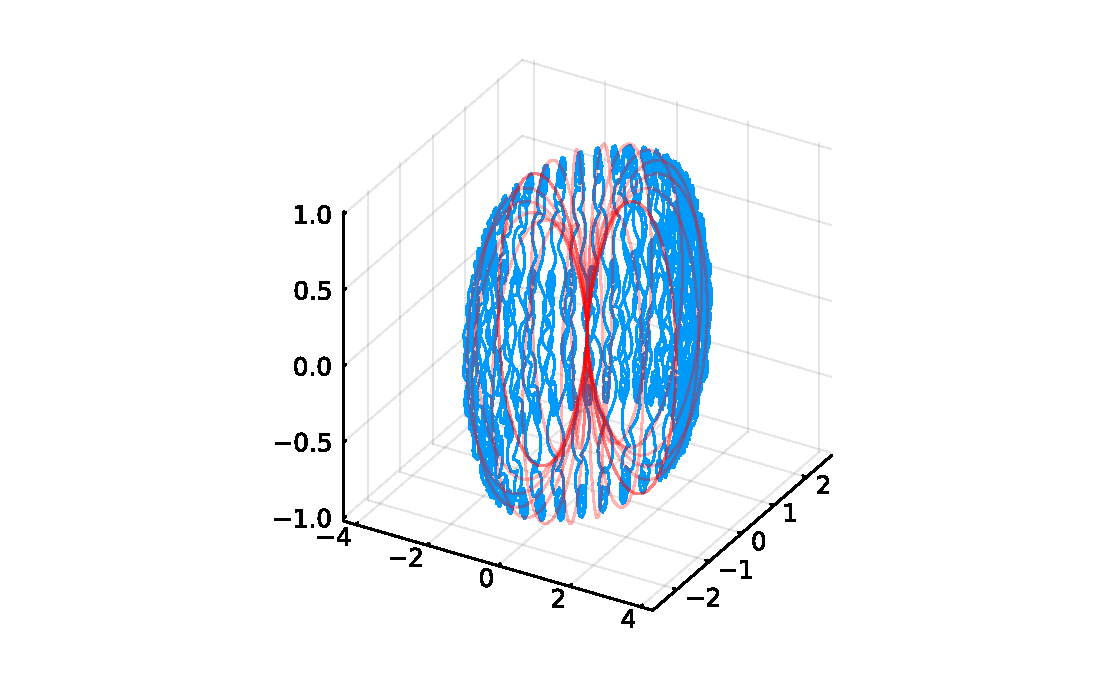
\includegraphics{./Dipolefield_Motion_files/figure-pdf/cell-9-output-1.pdf}

}

\end{figure}

\begin{Shaded}
\begin{Highlighting}[]
\NormalTok{p }\OperatorTok{=} \FunctionTok{plot\_iso3d}\NormalTok{(x, y, z, title}\OperatorTok{=}\StringTok{"Charged particle traces"}\NormalTok{)}
\NormalTok{p}
\end{Highlighting}
\end{Shaded}

\begin{figure}[H]

{\centering 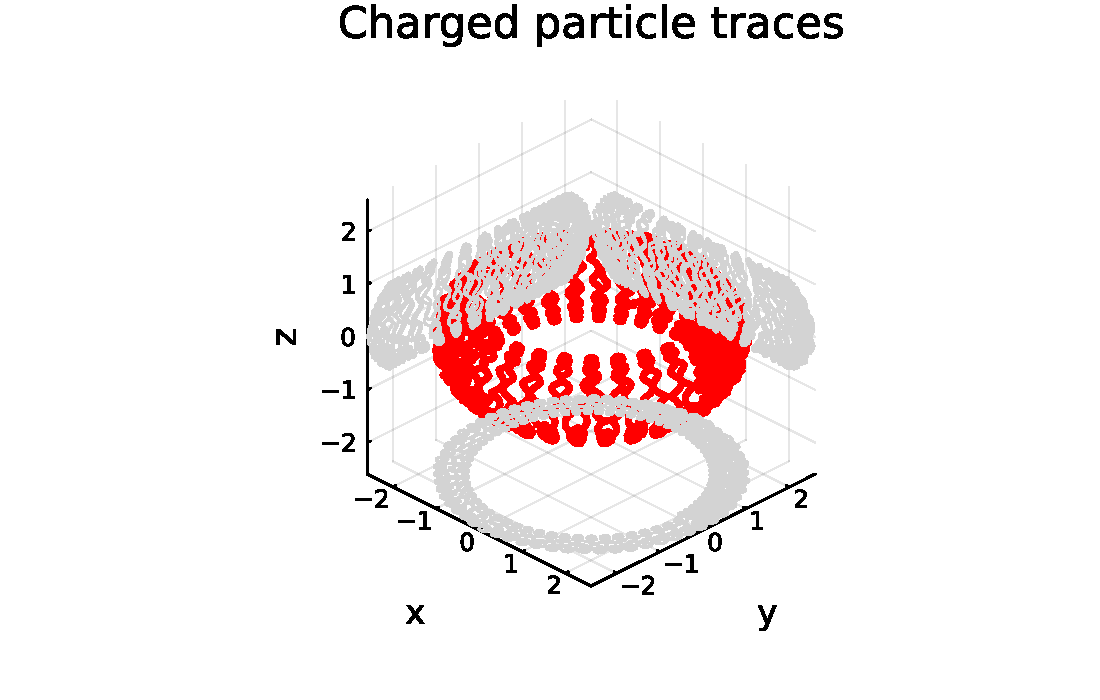
\includegraphics{./Dipolefield_Motion_files/figure-pdf/cell-10-output-1.pdf}

}

\end{figure}

\hypertarget{tutorial}{%
\chapter{Tutorial}\label{tutorial}}

Was die Analyse von Plasmen besonders schwierig macht, ist die Tatsache,
dass die Dichten in einem Zwischenbereich liegen. Flüssigkeiten wie
Wasser sind so dicht, dass die Bewegungen der einzelnen Moleküle nicht
berücksichtigt werden müssen. Es dominieren Kollisionen, und die
einfachen Gleichungen der gewöhnlichen Flüssigkeitsdynamik reichen aus.
Im anderen Extremfall, in Geräten mit sehr geringer Dichte, müssen nur
die Flugbahnen einzelner Teilchen berücksichtigt werden; kollektive
Effekte sind oft unwichtig. Ein Plasma verhält sich manchmal wie eine
Flüssigkeit und manchmal wie eine Ansammlung von Einzelteilchen. Der
erste Schritt, um zu lernen, wie man mit dieser schizophrenen
Persönlichkeit umgeht, besteht darin zu verstehen, wie sich einzelne
Teilchen in elektrischen und magnetischen Feldern verhalten.

Hier gehen wir davon aus, dass die EM-Felder vorgegeben sind und nicht
von den geladenen Teilchen beeinflusst werden. Die Materialien hier
lehnen sich eng an F.F.Chens
\href{https://link.springer.com/book/10.1007/978-3-319-22309-4}{Einführung
in die Plasmaphysik und kontrollierte Fusion} an.

In allen Beispielen gehen wir davon aus, dass die folgenden Pakete
geladen sind:

\begin{Shaded}
\begin{Highlighting}[]
\ImportTok{using} \BuiltInTok{JSServe}\NormalTok{: Page }\CommentTok{\# hide}
\FunctionTok{Page}\NormalTok{(exportable}\OperatorTok{=}\ConstantTok{true}\NormalTok{, offline}\OperatorTok{=}\ConstantTok{true}\NormalTok{) }\CommentTok{\# hide}
\end{Highlighting}
\end{Shaded}

\begin{verbatim}
Page(JSServe.Session(Base.RefValue{Union{Nothing, WebSockets.WebSocket, IOBuffer}}(nothing), Dict{String, Tuple{Bool, Observables.Observable}}(), Dict{Symbol, Any}[], Set{JSServe.Asset}(), JSServe.JSCode[], "31d0070e-baab-4e89-86ef-bfbf9cb488ea", Channel{Bool}(1), JSServe.init_session, JSServe.UrlSerializer(true, nothing, true, "http://localhost:9284", true), Base.RefValue{Union{Nothing, JSServe.JSException}}(nothing), Observable{Union{Nothing, Dict{String, Any}}}(nothing), Observable(false), Observables.ObserverFunction[], Dict{String, WeakRef}()), Dict{String, JSServe.Session}(), true, true)
\end{verbatim}

\begin{Shaded}
\begin{Highlighting}[]
\ImportTok{using} \BuiltInTok{TestParticle}
\ImportTok{using} \BuiltInTok{TestParticle}\NormalTok{: get\_gc}
\ImportTok{using} \BuiltInTok{TestParticleMakie}
\ImportTok{using} \BuiltInTok{OrdinaryDiffEq}
\ImportTok{using} \BuiltInTok{StaticArrays}
\ImportTok{using} \BuiltInTok{LinearAlgebra}
\ImportTok{import} \BuiltInTok{GLMakie }\NormalTok{as WM}
\end{Highlighting}
\end{Shaded}

\hypertarget{homogene-e--und-b-felder}{%
\section{Homogene E- und B-Felder}\label{homogene-e--und-b-felder}}

\hypertarget{e0}{%
\subsection{E=0}\label{e0}}

In diesem Fall führt ein geladenes Teilchen eine einfache
Gyrationsbewegung aus. Die Bewegungsgleichung lautet

\[
m\frac{\mathrm d\mathbf{v}}{\mathrm dt} = q\mathbf{v}\times\mathbf{B}
\]

Nimmt man \(\widehat{z}\) als die Richtung von \(\mathbf{B}\)
(\(\mathbf{B} = B\widehat{z}\)), so gilt

\[
\begin{aligned}
m\dot{v}_x = qB v_y,\, m\dot{v}_y = -qB v_x,\, m\dot{v}_z = 0, \\
\ddot{v}_x = \frac{qB}{m}\dot{v}_y = -\big( \frac{qB}{m}\big)^2 v_x \\
\ddot{v}_y = \frac{qB}{m}\dot{v}_x = -\big( \frac{qB}{m}\big)^2 v_y
\end{aligned}
\]

Dies beschreibt einen einfachen harmonischen Oszillator mit der
\emph{Gyrationsfrequenz}, die wir wie folgt definieren

\[
\omega_c \equiv \frac{| q | B}{m}
\]

Nach der von uns gewählten Konvention ist \(\omega_c\) immer
nicht-negativ. Die Lösung für die Geschwindigkeit ist dann

\[
v_{x,y} = v_\perp \exp(\pm i \omega_c t + i\delta_{x,y})
\]

Die \(\pm\) bezeichnen das Vorzeichen von q. Wir können die Phase
\(\delta\) so wählen, dass

\[
v_x = v_\perp e^{i\omega_c t} = \dot{x}
\]

wobei \(v_\perp\) eine positive Konstante ist, die die Geschwindigkeit
in der Ebene senkrecht zu \(\mathbf{B}\) angibt. Dann gilt

\[
v_y  = \frac{m}{qB} \dot{v}_x = \pm \frac{1}{\omega_c}\dot{v}_x = \pm i v_\perp e^{i\omega_c t} = \dot{y}
\]

Nochmalige Integration liefert

\[
\begin{aligned}
x - x_0 &= -i\frac{v_\perp}{\omega_c}e^{i\omega_c t} \\
y - y_0 &= \pm i\frac{v_\perp}{\omega_c}e^{i\omega_c t}
\end{aligned}
\]

Wir definieren die \emph{Gyrationsradius} zu

\[
r_L \equiv \frac{v_\perp}{\omega_c} = \frac{mv_\perp}{|q| B}
\]

Der Realteil liefert

\[
\begin{aligned}
x - x_0 &= r_L\sin\omega_c t \\
y - y_0 &= \pm r_L \cos\omega_c t  
\end{aligned} 
\]

Diese beschreibt eine Kreisbahn um ein \emph{Führungszentrum}
(\(x_0, y_0\)), das ortsfest ist. Die Richtung der Kreisbewegung ist
immer so, dass das von dem geladenen Teilchen erzeugte Magnetfeld dem
von außen angelegten Feld entgegengesetzt ist. Plasmateilchen neigen
daher dazu, das Magnetfeld zu \emph{schwächen}, und Plasmen sind
\emph{diamagnetisch}. Zusätzlich zu dieser Bewegung gibt es eine
beliebige Geschwindigkeit \(v_z\) entlang \(\mathbf{B}\), die von
\(\mathbf{B}\) nicht beeinflusst wird. Die Flugbahn eines geladenen
Teilchens im Raum ist im Allgemeinen eine Spirale.

\begin{Shaded}
\begin{Highlighting}[]
\KeywordTok{function} \FunctionTok{uniform\_B}\NormalTok{(x)}
    \ControlFlowTok{return}\NormalTok{ SA[}\FloatTok{0.0}\NormalTok{, }\FloatTok{0.0}\NormalTok{, }\FloatTok{1e{-}8}\NormalTok{]}
\KeywordTok{end}

\KeywordTok{function} \FunctionTok{uniform\_E}\NormalTok{(x)}
    \ControlFlowTok{return}\NormalTok{ SA[}\FloatTok{0.0}\NormalTok{, }\FloatTok{0.0}\NormalTok{, }\FloatTok{0.0}\NormalTok{]}
\KeywordTok{end}

\NormalTok{x0 }\OperatorTok{=}\NormalTok{ [}\FloatTok{1.0}\NormalTok{, }\FloatTok{0}\NormalTok{, }\FloatTok{0}\NormalTok{]}
\NormalTok{v0 }\OperatorTok{=}\NormalTok{ [}\FloatTok{0.0}\NormalTok{, }\FloatTok{1.0}\NormalTok{, }\FloatTok{0.1}\NormalTok{]}
\NormalTok{stateinit }\OperatorTok{=}\NormalTok{ [x0}\OperatorTok{...}\NormalTok{, v0}\OperatorTok{...}\NormalTok{]}
\NormalTok{tspan }\OperatorTok{=}\NormalTok{ (}\FloatTok{0}\NormalTok{, }\FloatTok{18}\NormalTok{)}

\NormalTok{param }\OperatorTok{=} \FunctionTok{prepare}\NormalTok{(uniform\_E, uniform\_B, species}\OperatorTok{=}\NormalTok{Proton)}
\NormalTok{prob }\OperatorTok{=} \FunctionTok{ODEProblem}\NormalTok{(trace!, stateinit, tspan, param)}
\NormalTok{sol }\OperatorTok{=} \FunctionTok{solve}\NormalTok{(prob, }\FunctionTok{Tsit5}\NormalTok{(); save\_idxs}\OperatorTok{=}\NormalTok{[}\FloatTok{1}\NormalTok{,}\FloatTok{2}\NormalTok{,}\FloatTok{3}\NormalTok{,}\FloatTok{4}\NormalTok{,}\FloatTok{5}\NormalTok{,}\FloatTok{6}\NormalTok{])}

\NormalTok{WM.}\FunctionTok{plot}\NormalTok{(sol)}
\end{Highlighting}
\end{Shaded}

\begin{figure}[H]

{\centering 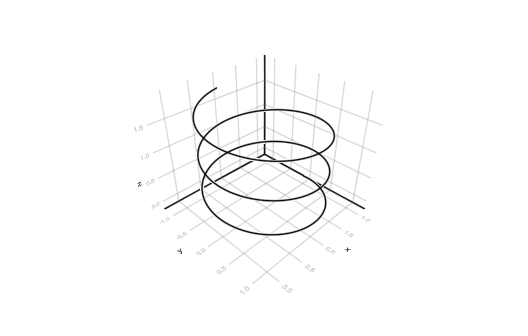
\includegraphics{./Tutorial_files/figure-pdf/cell-4-output-1.png}

}

\end{figure}

\hypertarget{e-feld}{%
\subsection{E-Feld}\label{e-feld}}

Wenn wir nun ein elektrisches Feld zulassen, ergibt sich die Bewegung
als Summe zweier Bewegungen: die kreisförmige Gyration und eine Drift
des Führungszentrums. Wir können \(\mathbf{E}\) so wählen, dass es in
der Ebene \(x\)-\(z\) liegt, so dass \(E_y = 0\) ist. Wie zuvor ist die
\(z\)-Komponente der Geschwindigkeit unabhängig von den transversalen
Komponenten und kann separat behandelt werden. Die Bewegungsgleichung
lautet nun

\[
m\frac{d\mathbf{v}}{dt} = q( \mathbf{E} + \mathbf{v}\times\mathbf{B} )
\]

dessen \(z\)-Komponente lautet

\[
\frac{dv_z}{dt} = \frac{q}{m}E_z
\]

oder

\[
v_z = \frac{qE_z}{m}t + v_{z0}
\]

Dies ist eine einfache Beschleunigung entlang \(\mathbf{B}\). Die
Komponenten senkrecht dazu sind

\[
\begin{aligned}
\frac{dv_x}{dt} &= \frac{q}{m}E_x \pm \omega_c v_y \\
\frac{dv_y}{dt} &= 0 \mp \omega_c v_x
\end{aligned}
\]

Nach Differentiation bei konstantem elektrischen Feld erhalten wir

\[
\begin{aligned}
\ddot{v}_x &= -\omega_c^2 v_x \\
\ddot{v}_y &= \mp \omega_c \Big( \frac{q}{m}E_x \pm \omega_c v_y \Big) = -\omega_c^2 \Big( v_y + \frac{E_x}{B} \Big)
\end{aligned}
\]

welches wir umschreiben

\[
\frac{d^2}{dt^2}\Big( v_y + \frac{E_x}{B} \Big) = -\omega_c^2\Big( v_y + \frac{E_x}{B} \Big)
\]

so dass es sich auf den vorherigen Fall reduziert, wenn wir \(v_y\)
durch \(v_y + (E_x/B)\) ersetzen. Die Geschwindigkeitslösung wird dann
ersetzt durch

\[
\begin{aligned}
v_x &= v_\perp e^{i\omega_c t} \\
v_y &= \pm v_\perp e^{i\omega_c t} - \frac{E_x}{B}
\end{aligned}
\]

Die Gyrationsbewegung ist dieselbe wie zuvor, aber es wird eine Drift
\(\mathbf{v}_{gc}\) des Führungszentrums in negative y-Richtung (für
\(E_x > 0\)) überlagert.

Um eine allgemeine Formel für \(\mathbf{v}_{gc}\) zu erhalten, können
wir die Impulsgleichung in Vektorform lösen. Wir können den Term
\(m d\mathbf{v}/dt\) weglassen, da dieser Term nur die Kreisbewegung bei
\(\omega_c\) ergibt, die wir bereits kennen. Die Impulsgleichung lautet
dann

\[
\mathbf{E} + \mathbf{v}\times\mathbf{B} = 0
\]

Nimmt man das Kreuzprodukt mit \(\mathbf{B}\), so erhält man

\[
\mathbf{E}\times\mathbf{B} = \mathbf{B}\times(\mathbf{v}\times\mathbf{B}) = \mathbf{v}B^2 - \mathbf{B}(\mathbf{v}\cdot\mathbf{B})
\]

Die zum Magnetfeld transversale Komponente dieser Gleichung lautet

\[
\mathbf{v}_{gc} = \mathbf{E}\times\mathbf{B}/B^2 \equiv \mathbf{v}_E
\]

Wir definieren dies als \(\mathbf{v}_E\), die durch das elektrische Feld
verursachte Drift des Führungszentrums. Der Größenordnung nach ist diese
Drift

\[
v_E = \frac{E(\text{V/m})}{B(\text{tesla})}\frac{\text{m}}{\text{sec}}
\]

Es ist wichtig zu beachten, dass \(\mathbf{v}_E\) unabhängig von q, m
und \(v_\perp\) ist. Der Grund dafür ergibt sich aus dem folgenden
physikalischen Bild. Im ersten Halbzyklus der Ionenbahn gewinnt das Ion
Energie aus dem elektrischen Feld und erhöht \(v_\perp\) und damit auch
\(r_L\). Im zweiten Halbzyklus verliert es Energie und nimmt in \(r_L\)
ab. Dieser Unterschied in \(r_L\) auf der linken und rechten Seite der
Bahn verursacht die Drift \(v_E\). Ein negatives Elektron dreht sich in
die entgegengesetzte Richtung, gewinnt aber auch Energie in die
entgegengesetzte Richtung; es driftet schließlich in dieselbe Richtung
wie ein Ion. Bei Teilchen mit gleicher Geschwindigkeit, aber
unterschiedlicher Masse, hat das leichtere Teilchen ein kleineres
\(r_L\) und driftet daher weniger pro Zyklus. Allerdings ist auch seine
Gyrationsfrequenz größer, und die beiden Effekte heben sich genau auf.
Zwei Teilchen mit gleicher Masse, aber unterschiedlicher Energie hätten
das gleiche \(\omega_c\). Das langsamere Teilchen hat ein kleineres
\(r_L\) und gewinnt daher weniger Energie aus \(\mathbf{E}\) in einem
Halbzyklus. Bei weniger energiereichen Teilchen ist jedoch der Anteil
der \(r_L\)-Änderung bei einer gegebenen Energieänderung größer, und
diese beiden Effekte heben sich auf.

Die dreidimensionale Umlaufbahn im Raum ist also eine schräge Helix mit
wechselnder Steigung.

\begin{Shaded}
\begin{Highlighting}[]
\KeywordTok{function} \FunctionTok{uniform\_B}\NormalTok{(x)}
    \ControlFlowTok{return}\NormalTok{ SA[}\FloatTok{0}\NormalTok{, }\FloatTok{0}\NormalTok{, }\FloatTok{1e{-}8}\NormalTok{]}
\KeywordTok{end}

\KeywordTok{function} \FunctionTok{uniform\_E}\NormalTok{(x)}
    \ControlFlowTok{return}\NormalTok{ SA[}\FloatTok{1e{-}9}\NormalTok{, }\FloatTok{0}\NormalTok{, }\FloatTok{0}\NormalTok{]}
\KeywordTok{end}

\CommentTok{\# trace the orbit of the guiding center}
\KeywordTok{function} \FunctionTok{trace\_gc!}\NormalTok{(dx, x, p, t)}
\NormalTok{    \_, \_, E, B, sol }\OperatorTok{=}\NormalTok{ p}
\NormalTok{    xu }\OperatorTok{=} \FunctionTok{sol}\NormalTok{(t)}
\NormalTok{    Bv }\OperatorTok{=} \FunctionTok{B}\NormalTok{(x)}
\NormalTok{    b }\OperatorTok{=} \FunctionTok{normalize}\NormalTok{(Bv)}
\NormalTok{    v\_par }\OperatorTok{=}\NormalTok{ (xu[}\FloatTok{4}\OperatorTok{:}\FloatTok{6}\NormalTok{]}\OperatorTok{⋅}\NormalTok{b)}\OperatorTok{.*}\NormalTok{b}
\NormalTok{    B2 }\OperatorTok{=} \FunctionTok{sum}\NormalTok{(Bv}\OperatorTok{.\^{}}\FloatTok{2}\NormalTok{)}
\NormalTok{    dx[}\FloatTok{1}\OperatorTok{:}\FloatTok{3}\NormalTok{] }\OperatorTok{=}\NormalTok{ (}\FunctionTok{E}\NormalTok{(x)}\OperatorTok{×}\NormalTok{Bv)}\OperatorTok{/}\NormalTok{B2 }\OperatorTok{+}\NormalTok{ v\_par}
\KeywordTok{end}

\NormalTok{x0 }\OperatorTok{=}\NormalTok{ [}\FloatTok{1.0}\NormalTok{, }\FloatTok{0}\NormalTok{, }\FloatTok{0}\NormalTok{]}
\NormalTok{v0 }\OperatorTok{=}\NormalTok{ [}\FloatTok{0.0}\NormalTok{, }\FloatTok{1.0}\NormalTok{, }\FloatTok{0.1}\NormalTok{]}
\NormalTok{stateinit }\OperatorTok{=}\NormalTok{ [x0}\OperatorTok{...}\NormalTok{, v0}\OperatorTok{...}\NormalTok{]}
\NormalTok{tspan }\OperatorTok{=}\NormalTok{ (}\FloatTok{0}\NormalTok{, }\FloatTok{20}\NormalTok{)}
\CommentTok{\# E×B drift}
\NormalTok{param }\OperatorTok{=} \FunctionTok{prepare}\NormalTok{(uniform\_E, uniform\_B, species}\OperatorTok{=}\NormalTok{Proton)}
\NormalTok{prob }\OperatorTok{=} \FunctionTok{ODEProblem}\NormalTok{(trace!, stateinit, tspan, param)}
\NormalTok{sol }\OperatorTok{=} \FunctionTok{solve}\NormalTok{(prob, }\FunctionTok{Tsit5}\NormalTok{(); save\_idxs}\OperatorTok{=}\NormalTok{[}\FloatTok{1}\NormalTok{,}\FloatTok{2}\NormalTok{,}\FloatTok{3}\NormalTok{,}\FloatTok{4}\NormalTok{,}\FloatTok{5}\NormalTok{,}\FloatTok{6}\NormalTok{])}

\NormalTok{gc }\OperatorTok{=} \FunctionTok{get\_gc}\NormalTok{(param)}
\NormalTok{gc\_x0 }\OperatorTok{=}\NormalTok{ [}\FunctionTok{gc\_i}\NormalTok{(stateinit) for gc\_i }\KeywordTok{in}\NormalTok{ gc]}
\NormalTok{prob\_gc }\OperatorTok{=} \FunctionTok{ODEProblem}\NormalTok{(trace\_gc!, gc\_x0, tspan, (param}\OperatorTok{...}\NormalTok{, sol))}
\NormalTok{sol\_gc }\OperatorTok{=} \FunctionTok{solve}\NormalTok{(prob\_gc, }\FunctionTok{Tsit5}\NormalTok{(); save\_idxs}\OperatorTok{=}\NormalTok{[}\FloatTok{1}\NormalTok{,}\FloatTok{2}\NormalTok{,}\FloatTok{3}\NormalTok{])}

\NormalTok{gc\_analytic }\OperatorTok{=} \FunctionTok{Tuple}\NormalTok{(xu }\OperatorTok{{-}\textgreater{}} \FunctionTok{getindex}\NormalTok{(}\FunctionTok{sol\_gc}\NormalTok{(xu[}\FloatTok{7}\NormalTok{]), i) }\ControlFlowTok{for}\NormalTok{ i }\OperatorTok{=} \FloatTok{1}\OperatorTok{:}\FloatTok{3}\NormalTok{)}
\CommentTok{\# numeric result and analytic result}
\FunctionTok{orbit}\NormalTok{(sol, vars}\OperatorTok{=}\NormalTok{[(}\FloatTok{1}\NormalTok{, }\FloatTok{2}\NormalTok{, }\FloatTok{3}\NormalTok{), gc, gc\_analytic])}
\end{Highlighting}
\end{Shaded}

\begin{figure}[H]

{\centering 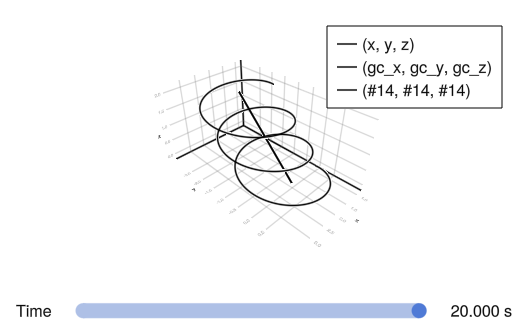
\includegraphics{./Tutorial_files/figure-pdf/cell-5-output-1.png}

}

\end{figure}

\hypertarget{schwerefeld}{%
\subsection{Schwerefeld}\label{schwerefeld}}

Das vorherige Ergebnis kann auf andere Kräfte übertragen werden, indem
\(q\mathbf{E}\) in der Bewegungsgleichung durch eine allgemeine Kraft
\(\mathbf{F}\) ersetzt wird. Die durch \(\mathbf{F}\) verursachte Drift
des Führungszentrums ist dann

\[
\mathbf{v}_f = \frac{1}{q}\frac{\mathbf{F}\times\mathbf{B}}{B^2}
\]

Insbesondere wenn \(\mathbf{F}\) die Schwerkraft \(m\mathbf{g}\) ist,
gibt es eine Drift

\[
\mathbf{v}_g = \frac{m}{q}\frac{\mathbf{g}\times\mathbf{B}}{B^2}
\]

Sie ähnelt der Drift \(\mathbf{v}_E\) insofern, als sie sowohl zur Kraft
als auch zu \(\mathbf{B}\) senkrecht steht, unterscheidet sich aber in
einem wichtigen Punkt. Die Drift \(\mathbf{v}_g\) ändert ihr Vorzeichen
mit der Ladung des Teilchens. Unter einer Gravitationskraft driften
Ionen und Elektronen in entgegengesetzte Richtungen, so dass sich im
Plasma eine Nettostromdichte ergibt, die durch

\[
\mathbf{j} = n(M+m)\frac{\mathbf{g}\times\mathbf{B}}{B^2}
\]

Der physikalische Grund für diese Drift ist wiederum die Änderung des
Larmor-Radius, wenn das Teilchen im Gravitationsfeld Energie gewinnt und
verliert. Jetzt drehen sich die Elektronen in die entgegengesetzte
Richtung wie die Ionen, aber die Kraft, die auf sie einwirkt, geht in
dieselbe Richtung, so dass die Drift in die entgegengesetzte Richtung
geht. Die Größe von \(\mathbf{v}_g\) ist normalerweise vernachlässigbar,
aber wenn die Kraftlinien (d.h. die Magnetfeldlinien) gekrümmt sind,
gibt es eine effektive Gravitationskraft aufgrund der Zentrifugalkraft.
Diese Kraft, die nicht vernachlässigbar ist, ist unabhängig von der
Masse; aus diesem Grund haben wir die m-Abhängigkeit der Drift hier
nicht betont. Die Zentrifugalkraft ist die Grundlage einer
Plasmainstabilität, der so genannten ``Gravitationsinstabilität'', die
nichts mit der realen Schwerkraft zu tun hat.

\begin{Shaded}
\begin{Highlighting}[]
\KeywordTok{function} \FunctionTok{B}\NormalTok{(x)}
    \ControlFlowTok{return}\NormalTok{ SA[}\FloatTok{0.0}\NormalTok{, }\FloatTok{1e{-}8}\NormalTok{, }\FloatTok{0.0}\NormalTok{]}
\KeywordTok{end}

\KeywordTok{function} \FunctionTok{E}\NormalTok{(x)}
    \ControlFlowTok{return}\NormalTok{ SA[}\FloatTok{0.0}\NormalTok{, }\FloatTok{0.0}\NormalTok{, }\FloatTok{0.0}\NormalTok{]}
\KeywordTok{end}
\CommentTok{\# gravity}
\KeywordTok{function} \FunctionTok{F}\NormalTok{(x)}
    \ControlFlowTok{return}\NormalTok{ SA[}\FloatTok{0.0}\NormalTok{, }\FloatTok{0.0}\NormalTok{, }\OperatorTok{{-}}\NormalTok{TestParticle.mᵢ}\OperatorTok{*}\FloatTok{9.8}\NormalTok{]}
\KeywordTok{end}
\CommentTok{\# initial static particle}
\NormalTok{x0 }\OperatorTok{=}\NormalTok{ [}\FloatTok{1.0}\NormalTok{, }\FloatTok{0}\NormalTok{, }\FloatTok{0}\NormalTok{]}
\NormalTok{v0 }\OperatorTok{=}\NormalTok{ [}\FloatTok{0.0}\NormalTok{, }\FloatTok{0.0}\NormalTok{, }\FloatTok{0.0}\NormalTok{]}
\NormalTok{stateinit }\OperatorTok{=}\NormalTok{ [x0}\OperatorTok{...}\NormalTok{, v0}\OperatorTok{...}\NormalTok{]}
\NormalTok{tspan }\OperatorTok{=}\NormalTok{ (}\FloatTok{0}\NormalTok{, }\FloatTok{1.0}\NormalTok{)}

\NormalTok{param }\OperatorTok{=} \FunctionTok{prepare}\NormalTok{(E, B, F, species}\OperatorTok{=}\NormalTok{Proton)}
\NormalTok{prob }\OperatorTok{=} \FunctionTok{ODEProblem}\NormalTok{(trace!, stateinit, tspan, param)}
\NormalTok{sol }\OperatorTok{=} \FunctionTok{solve}\NormalTok{(prob, }\FunctionTok{Tsit5}\NormalTok{(); save\_idxs}\OperatorTok{=}\NormalTok{[}\FloatTok{1}\NormalTok{,}\FloatTok{2}\NormalTok{,}\FloatTok{3}\NormalTok{])}
\CommentTok{\# drift in x{-}direction + free fall in z{-}direction}
\NormalTok{WM.}\FunctionTok{plot}\NormalTok{(sol)}
\end{Highlighting}
\end{Shaded}

\begin{figure}[H]

{\centering 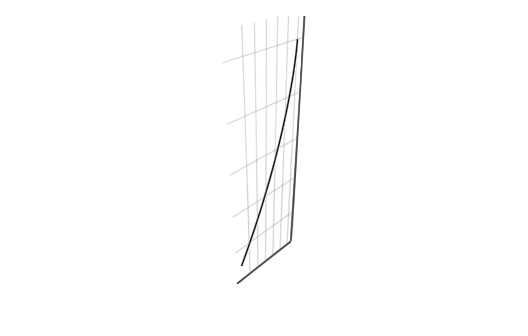
\includegraphics{./Tutorial_files/figure-pdf/cell-6-output-1.png}

}

\end{figure}

\hypertarget{inhomogenes-b-feld}{%
\section{Inhomogenes B-Feld}\label{inhomogenes-b-feld}}

Da das Konzept der Drift des Führungszentrums nun fest etabliert ist,
können wir die Bewegung von Teilchen in inhomogenen Feldern ---
\(\mathbf{E}\) und \(\mathbf{B}\) Feldern, die in Raum oder Zeit
variieren, diskutieren. Für gleichförmige Felder konnten wir exakte
Ausdrücke für die Drifts des Führungszentrums erhalten. Sobald wir
Inhomogenität einführen, wird das Problem zu kompliziert, um es exakt zu
lösen. Um eine ungefähre Antwort zu erhalten, ist es üblich, in dem
kleinen Verhältnis \(r_L/L\) zu expandieren, wobei L die Skalenlänge der
Inhomogenität ist. Diese Art von Theorie, die so genannte
\emph{Orbit-Theorie}, kann sehr kompliziert werden. Wir werden nur die
einfachsten Fälle untersuchen, in denen jeweils nur eine Inhomogenität
auftritt.

\hypertarget{b-b-grad-b-drift}{%
\subsection{∇B ⊥ B: Grad-B-Drift}\label{b-b-grad-b-drift}}

Hier sind die magnetischen Feldlinien nicht gekrümmt, aber ihre Dichte
nimmt z. B. in y-Richtung zu. Wir können das Ergebnis vorhersagen, indem
wir ein einfaches physikalisches Bild verwenden. Der Gradient in
\textbar B\textbar{} bewirkt, dass der Larmor-Radius am unteren Ende der
Bahn größer ist als am oberen Ende, und dies sollte zu einer Drift in
entgegengesetzte Richtungen für Ionen und Elektronen führen, die sowohl
senkrecht zu B als auch zu \(\nabla B\) verläuft. Die
Driftgeschwindigkeit sollte offensichtlich proportional zu \(r_L/L\) und
zu \(v_\perp\) sein.

Betrachten wir die Lorentz-Kraft
\(\mathbf{F} = q\mathbf{v}\times\mathbf{B}\), gemittelt über eine
Gyration. Es ist klar, dass \(\bar{F}_x = 0\) ist, da sich das Teilchen
genauso viel Zeit nach oben wie nach unten bewegt. Wir wollen
\(\bar{F}_y\) näherungsweise berechnen, indem wir die \emph{ungestörte
Bahn} des Teilchens verwenden, um den Durchschnitt zu finden. Die
ungestörte Bahn ist durch die Lösung im ersten Abschnitt für ein
gleichförmiges \(\mathbf{B}\)-Feld gegeben. Nimmt man den Realteil der
Lösung für \(v_x\) und \(y\), so erhält man

\[
F_y = -q v_x B_z(y) = -q v_\perp(\cos \omega_c t) \Big[ B_0 \pm r_L(\cos\omega_c t )\frac{\partial B}{\partial y} \Big]
\]

wobei wir eine Taylorentwicklung des Feldes \(\mathbf{B}\) um den Punkt
\(x_0=0, y_0=0\) durchgeführt haben

\[
\begin{aligned}
\mathbf{B} &= \mathbf{B}_0 + (\mathbf{r}\cdot\nabla)\mathbf{B} + ... \\
B_z &= B_0 + y(\partial B_z/\partial y) + ...
\end{aligned}
\]

Diese Entwicklung erfordert natürlich \(r_L / L \ll 1\), wobei L die
Längenskala von \(\partial Bz/\partial y\) ist. Der erste obige Term
geht bei einer Gyration im Durchschnitt gegen Null, und der Durchschnitt
von \(\cos^2 \omega_c t\) ist \(1/2\), so dass

\[
\bar{F}_y = \mp q v_\perp r_L \frac{1}{2}\frac{\partial B}{\partial y}
\]

Die Driftgeschwindigkeit des Führungszentrums beträgt dann

\[
\mathbf{v}_{gc} = \frac{1}{q}\frac{\mathbf{F}\times\mathbf{B}}{B^2} = \frac{1}{q}\frac{\bar{F}_y}{|B|}\widehat{x} = \mp \frac{v_\perp r_L}{B}\frac{1}{2} \frac{\partial B}{\partial y} \widehat{x}
\]

wobei wir die zuvor gezeigte Formel verwendet haben. Da die Wahl der
y-Achse willkürlich war, kann dies verallgemeinert werden zu

\[
\mathbf{v}_{\nabla B} = \pm v_\perp r_L \frac{\mathbf{B}\times \nabla B}{B^2}
\]

Dies hat alle Abhängigkeiten, die wir aus dem physikalischen Bild
erwartet haben; nur der Faktor \(\frac{1}{2}\) (der sich aus der
Mittelwertbildung ergibt) wurde nicht vorhergesagt. Man beachte, dass
\(\pm\) für das Vorzeichen der Ladung steht, und \(B\) für \(|B|\). Die
Größe \(\mathbf{v}_{\nabla B}\) wird als \emph{Grad-B-Drift} bezeichnet;
sie verläuft für Ionen und Elektronen in entgegengesetzter Richtung und
verursacht einen Strom quer zu \(\mathbf{B}\). Eine exakte Berechnung
von \(\mathbf{v}_{\nabla B}\) würde die Verwendung der exakten Bahn,
einschließlich der Drift, im Mittelungsprozess erfordern.

\begin{Shaded}
\begin{Highlighting}[]
\ImportTok{using} \BuiltInTok{ForwardDiff}\NormalTok{: gradient}

\KeywordTok{function} \FunctionTok{grad\_B}\NormalTok{(x)}
    \ControlFlowTok{return}\NormalTok{ SA[}\FloatTok{0}\NormalTok{, }\FloatTok{0}\NormalTok{, }\FloatTok{1e{-}8}\OperatorTok{+}\FloatTok{1e{-}9} \OperatorTok{*}\NormalTok{x[}\FloatTok{2}\NormalTok{]]}
\KeywordTok{end}

\KeywordTok{function} \FunctionTok{uniform\_E}\NormalTok{(x)}
    \ControlFlowTok{return}\NormalTok{ SA[}\FloatTok{1e{-}9}\NormalTok{, }\FloatTok{0}\NormalTok{, }\FloatTok{0}\NormalTok{]}
\KeywordTok{end}

\FunctionTok{abs\_B}\NormalTok{(x) }\OperatorTok{=} \FunctionTok{norm}\NormalTok{(}\FunctionTok{grad\_B}\NormalTok{(x))}

\CommentTok{\# trace the orbit of the guiding center}
\KeywordTok{function} \FunctionTok{trace\_gc!}\NormalTok{(dx, x, p, t)}
\NormalTok{    q, m, E, B, sol }\OperatorTok{=}\NormalTok{ p}
\NormalTok{    xu }\OperatorTok{=} \FunctionTok{sol}\NormalTok{(t)}
\NormalTok{    gradient\_B }\OperatorTok{=} \FunctionTok{gradient}\NormalTok{(abs\_B, x)}
\NormalTok{    Bv }\OperatorTok{=} \FunctionTok{B}\NormalTok{(x)}
\NormalTok{    b }\OperatorTok{=} \FunctionTok{normalize}\NormalTok{(Bv)}
\NormalTok{    v\_par }\OperatorTok{=}\NormalTok{ (xu[}\FloatTok{4}\OperatorTok{:}\FloatTok{6}\NormalTok{]}\OperatorTok{⋅}\NormalTok{b)}\OperatorTok{.*}\NormalTok{b}
\NormalTok{    v\_perp }\OperatorTok{=}\NormalTok{ xu[}\FloatTok{4}\OperatorTok{:}\FloatTok{6}\NormalTok{] }\OperatorTok{{-}}\NormalTok{ v\_par}
\NormalTok{    dx[}\FloatTok{1}\OperatorTok{:}\FloatTok{3}\NormalTok{] }\OperatorTok{=} \FunctionTok{m*norm}\NormalTok{(v\_perp)}\OperatorTok{\^{}}\FloatTok{2}\FunctionTok{*}\NormalTok{(Bv}\OperatorTok{×}\NormalTok{gradient\_B)}\OperatorTok{/}\NormalTok{(}\FloatTok{2}\FunctionTok{*q*norm}\NormalTok{(Bv)}\OperatorTok{\^{}}\FloatTok{3}\NormalTok{) }\OperatorTok{+}\NormalTok{ (}\FunctionTok{E}\NormalTok{(x)}\OperatorTok{×}\NormalTok{Bv)}\OperatorTok{/}\FunctionTok{norm}\NormalTok{(Bv)}\OperatorTok{\^{}}\FloatTok{2}\OperatorTok{+}\NormalTok{v\_par}
\KeywordTok{end}

\NormalTok{x0 }\OperatorTok{=}\NormalTok{ [}\FloatTok{1.0}\NormalTok{, }\FloatTok{0}\NormalTok{, }\FloatTok{0}\NormalTok{]}
\NormalTok{v0 }\OperatorTok{=}\NormalTok{ [}\FloatTok{0.0}\NormalTok{, }\FloatTok{1.0}\NormalTok{, }\FloatTok{0.1}\NormalTok{]}
\NormalTok{stateinit }\OperatorTok{=}\NormalTok{ [x0}\OperatorTok{...}\NormalTok{, v0}\OperatorTok{...}\NormalTok{]}
\NormalTok{tspan }\OperatorTok{=}\NormalTok{ (}\FloatTok{0}\NormalTok{, }\FloatTok{20}\NormalTok{)}
\NormalTok{param }\OperatorTok{=} \FunctionTok{prepare}\NormalTok{(uniform\_E, grad\_B, species}\OperatorTok{=}\NormalTok{Proton)}
\NormalTok{prob }\OperatorTok{=} \FunctionTok{ODEProblem}\NormalTok{(trace!, stateinit, tspan, param)}
\NormalTok{sol }\OperatorTok{=} \FunctionTok{solve}\NormalTok{(prob, }\FunctionTok{Tsit5}\NormalTok{(); save\_idxs}\OperatorTok{=}\NormalTok{[}\FloatTok{1}\NormalTok{,}\FloatTok{2}\NormalTok{,}\FloatTok{3}\NormalTok{,}\FloatTok{4}\NormalTok{,}\FloatTok{5}\NormalTok{,}\FloatTok{6}\NormalTok{])}

\NormalTok{gc }\OperatorTok{=} \FunctionTok{get\_gc}\NormalTok{(param)}
\NormalTok{gc\_x0 }\OperatorTok{=}\NormalTok{ [}\FunctionTok{gc\_i}\NormalTok{(stateinit) for gc\_i }\KeywordTok{in}\NormalTok{ gc]}
\NormalTok{prob\_gc }\OperatorTok{=} \FunctionTok{ODEProblem}\NormalTok{(trace\_gc!, gc\_x0, tspan, (param}\OperatorTok{...}\NormalTok{, sol))}
\NormalTok{sol\_gc }\OperatorTok{=} \FunctionTok{solve}\NormalTok{(prob\_gc, }\FunctionTok{Tsit5}\NormalTok{(); save\_idxs}\OperatorTok{=}\NormalTok{[}\FloatTok{1}\NormalTok{,}\FloatTok{2}\NormalTok{,}\FloatTok{3}\NormalTok{])}

\NormalTok{gc\_analytic }\OperatorTok{=} \FunctionTok{Tuple}\NormalTok{(xu }\OperatorTok{{-}\textgreater{}} \FunctionTok{getindex}\NormalTok{(}\FunctionTok{sol\_gc}\NormalTok{(xu[}\FloatTok{7}\NormalTok{]), i) }\ControlFlowTok{for}\NormalTok{ i }\OperatorTok{=} \FloatTok{1}\OperatorTok{:}\FloatTok{3}\NormalTok{)}
\CommentTok{\# numeric result and analytic result}
\CommentTok{\# The orbit of guiding center includes some high order terms, which is different from the}
\CommentTok{\# formula of magnetic field gradient drift of some textbooks that just preserves the first}
\CommentTok{\# order term.}
\FunctionTok{orbit}\NormalTok{(sol, vars}\OperatorTok{=}\NormalTok{[(}\FloatTok{1}\NormalTok{, }\FloatTok{2}\NormalTok{, }\FloatTok{3}\NormalTok{), gc, gc\_analytic])}
\end{Highlighting}
\end{Shaded}

\begin{figure}[H]

{\centering 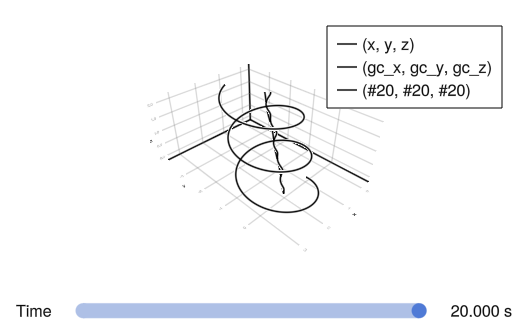
\includegraphics{./Tutorial_files/figure-pdf/cell-7-output-1.png}

}

\end{figure}

\hypertarget{gekruxfcmmte-feldlinien-kruxfcmmungsdrift}{%
\subsection{Gekrümmte Feldlinien:
Krümmungsdrift}\label{gekruxfcmmte-feldlinien-kruxfcmmungsdrift}}

Hier nehmen wir an, dass die magnetischen Feldlinien mit einem
konstanten Krümmungsradius \(R_c\) gekrümmt sind, und wir nehmen an,
dass \(|B|\) konstant ist. Ein solches Feld gehorcht im Vakuum nicht den
Maxwellschen Gleichungen, so dass in der Praxis die Grad-B-Drift immer
zu dem hier abgeleiteten Effekt hinzukommt. Eine Drift des
Führungszentrums entsteht durch die Zentrifugalkraft, die die Teilchen
spüren, wenn sie sich bei ihrer thermischen Bewegung entlang der
Feldlinien bewegen. Wenn \(v_\parallel^2\) das durchschnittliche Quadrat
der Komponente der Zufallsgeschwindigkeit entlang \(\mathbf{B}\)
bezeichnet, beträgt die durchschnittliche Zentrifugalkraft

\[
\mathbf{F}_{cf} = \frac{mv_\parallel^2}{R_c}\widehat{r} = mv_\parallel^2\frac{\mathbf{R}_c}{R_c^2}
\]

Nach der Formel für die Drift des Führungszentrums ergibt sich daraus
eine Drift

\[
\mathbf{v}_{R} = \frac{1}{q}\frac{\mathbf{F}_{cf}\times\mathbf{B}}{B^2} = \frac{mv_\parallel^2}{qB^2}\frac{\mathbf{R}_c \times\mathbf{B}}{R_c^2}
\]

Die Drift \(\mathbf{v}_R\) wird als \emph{Krümmungsdrift} bezeichnet.

Wir müssen nun die Grad-B-Drift berechnen, die damit einhergeht, wenn
die Abnahme von \(|B|\) mit dem Radius berücksichtigt wird. Im Vakuum
haben wir \(\nabla\times\mathbf{B} = 0\). In Zylinderkoordinaten hat
\(\nabla\times\mathbf{B}\) nur eine \(z\)-Komponente, da \(\mathbf{B}\)
nur eine \(\theta\)-Komponente und \(\nabla B\) nur eine
\(r\)-Komponente hat. Wir haben dann

\[
(\nabla\times\mathbf{B})_z = \frac{1}{r}\frac{\partial}{\partial r}(rB_\theta) = 0,\, B\propto \frac{1}{r}
\]

Deshalb

\[
|B| \propto \frac{1}{R_c},\, \frac{\nabla B}{B} = - \frac{\mathbf{R}_c}{R_c^2}
\] Unter Verwendung des Ausdrucks für die Grad-B-Drift ergibt sich

\[
\mathbf{v}_{\nabla B} = \mp \frac{1}{2}\frac{v_\perp r_L}{B^2}\frac{B}\times |B| \frac{\mathbf{R}_c}{R_c^2} = \pm \frac{1}{2}\frac{v_\perp^2}{\omega_c}\frac{\mathbf{R}_c\times\mathbf{B}}{R_c^2 B} = \frac{1}{2}\frac{m}{q}v_\perp^2\frac{\mathbf{R}_c\times\mathbf{B}}{R_c^2 B^2}
\]

Addiert man dies zu \(\mathbf{v}_R\) , so erhält man die Gesamtdrift in
einem gekrümmten Vakuumfeld:

\[
\mathbf{v}_R + \mathbf{v}_{\nabla B} = \frac{m}{q}\frac{\mathbf{R}_c\times\mathbf{B}}{R_c^2 B^2}\Big( v_\parallel^2 + \frac{1}{2}v_\perp^2 \Big)
\]

Bedauerlicherweise addieren sich diese Drifts. Das bedeutet, dass, wenn
man ein Magnetfeld in einen Torus biegt, um ein thermonukleares Plasma
einzuschließen, die Teilchen aus dem Torus herausdriften werden, egal
wie man mit den Temperaturen und Magnetfeldern jongliert.

Für eine Maxwellsche Verteilung sind \(\bar{v_\parallel^2}\) und
\(\frac{1}{2}\bar{v_\perp^2}\) jeweils gleich \(k_B T/m\), da
\(v_\perp\) zwei Freiheitsgrade beinhaltet. Dann kann die
durchschnittliche Drift des gekrümmten Feldes wie folgt geschrieben
werden

\[
\bar{\mathbf{v}}_{R+\nabla B} = \pm \frac{v_{th}^2}{R_c\omega_c}\widehat{y} = \pm\frac{\bar{r}_L}{R_c}v_{th}\widehat{y}
\]

wobei \(\widehat{y}\) hier die Richtung von
\(\widehat{R}_c\times\mathbf{B}\) ist. Dies zeigt, dass
\(\bar{\mathbf{v}}_{R+\nabla B}\) von der Ladung der Spezies abhängt,
aber nicht von ihrer Masse.

\begin{Shaded}
\begin{Highlighting}[]
\ImportTok{using} \BuiltInTok{ForwardDiff}\NormalTok{: gradient, jacobian}

\KeywordTok{function} \FunctionTok{curved\_B}\NormalTok{(x)}
    \CommentTok{\# satisify ∇⋅B=0}
    \CommentTok{\# B\_θ = 1/r =\textgreater{} ∂B\_θ/∂θ = 0}
\NormalTok{    θ }\OperatorTok{=} \FunctionTok{atan}\NormalTok{(x[}\FloatTok{3}\NormalTok{]}\OperatorTok{/}\NormalTok{(x[}\FloatTok{1}\NormalTok{]}\OperatorTok{+}\FloatTok{3}\NormalTok{))}
\NormalTok{    r }\OperatorTok{=} \FunctionTok{hypot}\NormalTok{(x[}\FloatTok{1}\NormalTok{]}\OperatorTok{+}\FloatTok{3}\NormalTok{, x[}\FloatTok{3}\NormalTok{])}
    \ControlFlowTok{return}\NormalTok{ SA[}\FunctionTok{{-}1e{-}7*sin}\NormalTok{(θ)}\OperatorTok{/}\NormalTok{r, }\FloatTok{0}\NormalTok{, }\FloatTok{1e{-}7}\FunctionTok{*cos}\NormalTok{(θ)}\OperatorTok{/}\NormalTok{r]}
\KeywordTok{end}

\KeywordTok{function} \FunctionTok{zero\_E}\NormalTok{(x)}
    \ControlFlowTok{return}\NormalTok{ SA[}\FloatTok{0}\NormalTok{, }\FloatTok{0}\NormalTok{, }\FloatTok{0}\NormalTok{]}
\KeywordTok{end}

\FunctionTok{abs\_B}\NormalTok{(x) }\OperatorTok{=} \FunctionTok{norm}\NormalTok{(}\FunctionTok{curved\_B}\NormalTok{(x))  }\CommentTok{\# |B|}

\CommentTok{\# trace the orbit of the guiding center}
\KeywordTok{function} \FunctionTok{trace\_gc!}\NormalTok{(dx, x, p, t)}
\NormalTok{    q, m, E, B, sol }\OperatorTok{=}\NormalTok{ p}
\NormalTok{    xu }\OperatorTok{=} \FunctionTok{sol}\NormalTok{(t)}
\NormalTok{    gradient\_B }\OperatorTok{=} \FunctionTok{gradient}\NormalTok{(abs\_B, x)  }\CommentTok{\# ∇|B|}
\NormalTok{    Bv }\OperatorTok{=} \FunctionTok{B}\NormalTok{(x)}
\NormalTok{    b }\OperatorTok{=} \FunctionTok{normalize}\NormalTok{(Bv)}
\NormalTok{    v\_par }\OperatorTok{=}\NormalTok{ (xu[}\FloatTok{4}\OperatorTok{:}\FloatTok{6}\NormalTok{]}\OperatorTok{⋅}\NormalTok{b)}\OperatorTok{.*}\NormalTok{b  }\CommentTok{\# (v⋅b)b}
\NormalTok{    v\_perp }\OperatorTok{=}\NormalTok{ xu[}\FloatTok{4}\OperatorTok{:}\FloatTok{6}\NormalTok{] }\OperatorTok{{-}}\NormalTok{ v\_par}
\NormalTok{    Ω }\OperatorTok{=} \FunctionTok{q*norm}\NormalTok{(Bv)}\OperatorTok{/}\NormalTok{m}
\NormalTok{    κ }\OperatorTok{=} \FunctionTok{jacobian}\NormalTok{(B, x)}\OperatorTok{*}\NormalTok{Bv  }\CommentTok{\# B⋅∇B}
    \CommentTok{\# v⟂\^{}2*(B×∇|B|)/(2*Ω*B\^{}2) + v∥\^{}2*(B×(B⋅∇B))/(Ω*B\^{}3) + (E×B)/B\^{}2 + v∥}
\NormalTok{    dx[}\FloatTok{1}\OperatorTok{:}\FloatTok{3}\NormalTok{] }\OperatorTok{=} \FunctionTok{norm}\NormalTok{(v\_perp)}\OperatorTok{\^{}}\FloatTok{2}\FunctionTok{*}\NormalTok{(Bv}\OperatorTok{×}\NormalTok{gradient\_B)}\OperatorTok{/}\NormalTok{(}\FloatTok{2}\FunctionTok{*Ω*norm}\NormalTok{(Bv)}\OperatorTok{\^{}}\FloatTok{2}\NormalTok{) }\OperatorTok{+} 
                \FunctionTok{norm}\NormalTok{(v\_par)}\OperatorTok{\^{}}\FloatTok{2}\FunctionTok{*}\NormalTok{(Bv}\OperatorTok{×}\NormalTok{κ)}\OperatorTok{/}\NormalTok{Ω}\OperatorTok{/}\FunctionTok{norm}\NormalTok{(Bv)}\OperatorTok{\^{}}\FloatTok{3} \OperatorTok{+}\NormalTok{ (}\FunctionTok{E}\NormalTok{(x)}\OperatorTok{×}\NormalTok{Bv)}\OperatorTok{/}\FunctionTok{norm}\NormalTok{(Bv)}\OperatorTok{\^{}}\FloatTok{2} \OperatorTok{+}\NormalTok{ v\_par}
\KeywordTok{end}

\NormalTok{x0 }\OperatorTok{=}\NormalTok{ [}\FloatTok{1.0}\NormalTok{, }\FloatTok{0}\NormalTok{, }\FloatTok{0}\NormalTok{]}
\NormalTok{v0 }\OperatorTok{=}\NormalTok{ [}\FloatTok{0.0}\NormalTok{, }\FloatTok{1.0}\NormalTok{, }\FloatTok{0.1}\NormalTok{]}
\NormalTok{stateinit }\OperatorTok{=}\NormalTok{ [x0}\OperatorTok{...}\NormalTok{, v0}\OperatorTok{...}\NormalTok{]}
\NormalTok{tspan }\OperatorTok{=}\NormalTok{ (}\FloatTok{0}\NormalTok{, }\FloatTok{40}\NormalTok{)}
\CommentTok{\# E×B drift}
\NormalTok{param }\OperatorTok{=} \FunctionTok{prepare}\NormalTok{(zero\_E, curved\_B, species}\OperatorTok{=}\NormalTok{Proton)}
\NormalTok{prob }\OperatorTok{=} \FunctionTok{ODEProblem}\NormalTok{(trace!, stateinit, tspan, param)}
\NormalTok{sol }\OperatorTok{=} \FunctionTok{solve}\NormalTok{(prob, }\FunctionTok{Tsit5}\NormalTok{(); save\_idxs}\OperatorTok{=}\NormalTok{[}\FloatTok{1}\NormalTok{,}\FloatTok{2}\NormalTok{,}\FloatTok{3}\NormalTok{,}\FloatTok{4}\NormalTok{,}\FloatTok{5}\NormalTok{,}\FloatTok{6}\NormalTok{])}

\NormalTok{gc }\OperatorTok{=} \FunctionTok{get\_gc}\NormalTok{(param)}
\NormalTok{gc\_x0 }\OperatorTok{=}\NormalTok{ [}\FunctionTok{gc\_i}\NormalTok{(stateinit) for gc\_i }\KeywordTok{in}\NormalTok{ gc]}
\NormalTok{prob\_gc }\OperatorTok{=} \FunctionTok{ODEProblem}\NormalTok{(trace\_gc!, gc\_x0, tspan, (param}\OperatorTok{...}\NormalTok{, sol))}
\NormalTok{sol\_gc }\OperatorTok{=} \FunctionTok{solve}\NormalTok{(prob\_gc, }\FunctionTok{Tsit5}\NormalTok{(); save\_idxs}\OperatorTok{=}\NormalTok{[}\FloatTok{1}\NormalTok{,}\FloatTok{2}\NormalTok{,}\FloatTok{3}\NormalTok{])}

\NormalTok{gc\_analytic }\OperatorTok{=} \FunctionTok{Tuple}\NormalTok{(xu }\OperatorTok{{-}\textgreater{}} \FunctionTok{getindex}\NormalTok{(}\FunctionTok{sol\_gc}\NormalTok{(xu[}\FloatTok{7}\NormalTok{]), i) }\ControlFlowTok{for}\NormalTok{ i }\OperatorTok{=} \FloatTok{1}\OperatorTok{:}\FloatTok{3}\NormalTok{)}
\CommentTok{\# numeric result and analytic result}
\CommentTok{\# similar to the magnetic field gradient drift}
\CommentTok{\# analytic calculation should include both of the gradient drift and the curvature drift}
\FunctionTok{orbit}\NormalTok{(sol, vars}\OperatorTok{=}\NormalTok{[(}\FloatTok{1}\NormalTok{, }\FloatTok{2}\NormalTok{, }\FloatTok{3}\NormalTok{), gc, gc\_analytic])}
\end{Highlighting}
\end{Shaded}

\begin{figure}[H]

{\centering 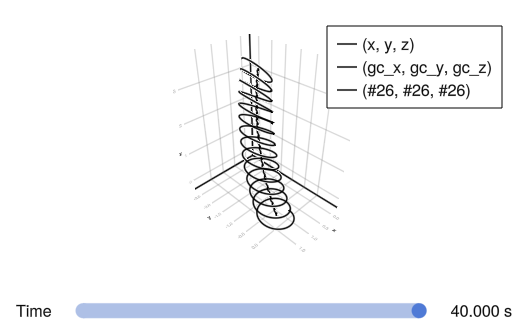
\includegraphics{./Tutorial_files/figure-pdf/cell-8-output-1.png}

}

\end{figure}

\hypertarget{b-b-magnetischer-spiegel}{%
\subsection{∇B ∥ B: Magnetischer
Spiegel}\label{b-b-magnetischer-spiegel}}

Wir betrachten nun ein Magnetfeld, das hauptsächlich in z-Richtung
gerichtet ist und dessen Größe in z-Richtung variiert. Das Feld sei
axialsymmetrisch, mit \(B_\theta = 0\) und
\(\partial/\partial\theta = 0\). Da die Magnetfeldlinien konvergieren
und divergieren, gibt es notwendigerweise eine Komponente \(B_r\). Wir
wollen zeigen, dass daraus eine Kraft resultiert, die ein Teilchen in
einem Magnetfeld einfangen kann.

Wir können \(B_r\) aus \(\nabla\cdot\mathbf{B} = 0\) erhalten:

\[
\frac{1}{r}\frac{\partial}{\partial r}(rB_r) + \frac{\partial B_z}{\partial z} = 0
\]

Wenn \(\mathbf{B}_z/\partial z\) bei \(r=0\) gegeben ist und nicht stark
mit r variiert, haben wir ungefähr

\[
\begin{aligned}
rB_r &= -\int_0^r r\frac{\partial B_z}{\partial z}dr \simeq -\frac{1}{2}r^2 \Big[ \frac{\partial \mathbf{B}_z}{\partial z} \Big]_{r=0} \\
B_r &= -\frac{1}{2}r \Big[ \frac{\partial \mathbf{B}_z}{\partial z} \Big]_{r=0}
\end{aligned}
\]

Die Variation von \(|B|\) mit r bewirkt eine grad-B-Drift der
Führungszentren um die Symmetrieachse, aber es gibt keine radiale
grad-B-Drift, weil \(\partial B/\partial \theta = 0\). Die Komponenten
der Lorentzkraft sind

\[
\newcommand{\textcircled}[1]{\enclose{circle}{\kern.1em\text{#1}\kern.1em}}
\begin{aligned}
F_r &= q(\underbrace{v_\theta B_z}_{\textcircled{\small{1}}} - v_z \cancel{B_\theta}) \\
F_\theta &= q(\underbrace{-v_r B_z}_{\textcircled{\small{2}}} + \underbrace{v_z B_r}_{\textcircled{\small{3}}}) \\
F_z &= q(v_r \cancel{B}_\theta - \underbrace{v_\theta B_r}_{\textcircled{\small{4}}})
\end{aligned}
\]

Zwei Terme verschwinden, wenn \(B_\theta = 0\) ist, und die Terme 1 und
2 bewirken die übliche Larmor-Gyration. Term 3 verschwindet auf der
Achse; wenn er nicht verschwindet, verursacht diese azimutale Kraft eine
Drift in radialer Richtung. Diese Drift führt lediglich dazu, dass die
Führungszentren den Magnetfeldlinien folgen. Term 4 ist derjenige, für
den wir uns interessieren. Unter Verwendung des Ausdrucks für \(B_r\)
ergibt sich

\[
F_z = \frac{1}{2}q v_\theta r_L \frac{\partial B_z}{\partial z}
\]

Wir müssen nun den Durchschnitt über eine Gyration bilden. Der
Einfachheit halber betrachten wir ein Teilchen, dessen Führungszentrum
auf der Achse liegt. Dann ist \(v_\theta\) eine Konstante während einer
Gyration; je nach Vorzeichen von q ist \(v_\theta\) gleich
\(\mp v_\perp\). Da \(r = r_L\) , ist die mittlere Kraft

\[
\bar{F}_z = \mp \frac{1}{2}q v_\perp r_L \frac{\partial B_z}{\partial z} = \mp \frac{1}{2}q\frac{v_\perp^2}{\omega_c} \frac{\partial B_z}{\partial z} = -\frac{1}{2}\frac{mv_\perp^2}{B} \frac{\partial B_z}{\partial z}
\]

Wir definieren das \emph{magnetische Moment} des kreisenden Teilchens
wie folgt

\[
\mu \equiv \frac{1}{2}mv_\perp^2 / B
\]

so dass

\[
\bar{F}_z = -\mu \frac{\partial B_z}{\partial z}
\]

Dies ist ein spezifisches Beispiel für die Kraft, die auf ein
diamagnetisches Teilchen einwirkt und die sich im Allgemeinen wie folgt
berechnen lässt

\[
\mathbf{F}_\parallel = -\mu\frac{\partial B}{\partial \mathbf{s}} = -\mu\nabla_\parallel B
\]

wobei \(d\mathbf{s}\) ein Linienelement entlang \(\mathbf{B}\) ist. Man
beachte, dass die Definition des magnetischen Moments hier dieselbe ist
wie die übliche Definition für das magnetische Moment einer
Stromschleife mit der Fläche A und dem Strom I: \(\mu = IA\). Im Falle
eines einfach geladenen Ions wird I durch eine Ladung e erzeugt, die
\(\omega_c / 2\pi\) mal pro Sekunde umläuft: \(I = e\omega_c/2\pi\). Die
Fläche A ist \(\pi r_L^2 = \pi r_L^2/\omega_c^2\). Also

\[
\mu = \frac{e\omega_c}{2\pi}\frac{\pi r_L^2}{\omega_c^2} = \frac{1}{2}\frac{v_\perp^2 e}{\omega_c} = \frac{1}{2}\frac{mv_\perp^2}{B}
\]

Wenn sich das Teilchen in Regionen mit stärkerem oder schwächerem B
bewegt, ändert sich sein Larmor-Radius, aber \emph{μ bleibt invariant}.
Um dies zu beweisen, betrachten wir die Komponente der
Bewegungsgleichung entlang \(\mathbf{B}\):

\[
m\frac{dv_\parallel}{dt} = -\mu \frac{\partial B}{\partial s}
\]

Durch Multiplikation mit \(v_\parallel\) auf der linken Seite und seinem
Äquivalent \(ds/dt\) auf der rechten Seite erhalten wir

\[
mv_\parallel \frac{dv_\parallel}{dt} = \frac{d}{dt}\Big( \frac{1}{2}mv_\parallel^2 \Big) = -\mu\frac{\partial B}{\partial s}\frac{ds}{dt} = -\mu\frac{dB}{dt}
\]

Dabei ist dB/dt die Veränderung von B aus der Sicht des Teilchens; B
selbst ist konstant. Die Energie des Teilchens muss erhalten bleiben,
also gilt

\[
\frac{d}{dt}\Big( \frac{1}{2}mv_\parallel^2 + \frac{1}{2}mv_\perp^2 \Big) = \frac{d}{dt}\Big( \frac{1}{2}mv_\parallel^2 + \mu B \Big) = 0
\]

Mit der vorhergehenden Gleichung ergibt sich

\[
-\mu\frac{dB}{dt} + \frac{d}{dt}(\mu B) = 0
\]

so dass

\[
\frac{d\mu}{dt} = 0
\]

Die Invarianz von \(\mu\) ist die Grundlage für eines der wichtigsten
Systeme für den Plasmaeinschluss: den \emph{magnetischen Spiegel}. Wenn
sich ein Teilchen im Laufe seiner thermischen Bewegung von einem Bereich
mit schwachem Feld zu einem Bereich mit starkem Feld bewegt, sieht es
ein zunehmendes B, und daher muss sein \(v_\perp\) zunehmen, um μ
konstant zu halten. Da seine Gesamtenergie konstant bleiben muss, muss
\(v_\parallel\) zwangsläufig abnehmen. Wenn B in der ``Kehle'' des
Spiegels hoch genug ist, wird \(v_\parallel\) schließlich zu Null; und
das Teilchen wird in den Bereich des schwachen Feldes
``zurückgeworfen''. Es ist natürlich die Kraft \(\mathbf{F}_\parallel\),
die die Reflexion verursacht. Das ungleichmäßige Feld eines einfachen
Spulenpaares bildet zwei Magnetspiegel, zwischen denen ein Plasma
gefangen werden kann. Dieser Effekt funktioniert sowohl bei Ionen als
auch bei Elektronen.

Das Einfangen ist jedoch nicht perfekt. Ein Teilchen mit \(v_\perp = 0\)
hat zum Beispiel kein magnetisches Moment und spürt keine Kraft entlang
\(\mathbf{B}\). Ein Teilchen mit kleinem \(v_\perp / v_\parallel\) in
der Mittelebene (\(B = B_0\)) wird ebenfalls entkommen, wenn das
maximale Feld \(B_m\) nicht groß genug ist. Welche Teilchen werden bei
gegebenem \(B_0\) und \(B_m\) entkommen? Ein Teilchen mit
\(v_\perp = v_{\perp 0}\) und \(v_\parallel = v_{\parallel 0}\) in der
Mittelebene hat \(v_\perp = v_\perp^\prime\) und \(v_\parallel = 0\) an
seinem Wendepunkt. Das Feld sei dort \(B^\prime\). Dann ergibt die
Invariante von \(\mu\)

\[
\frac{1}{2}\frac{mv_{\perp 0}^2}{B_0} = \frac{1}{2}\frac{m{v_{\perp 0}^{\prime}}^2}{B^\prime}
\]

Die Energieerhaltung erfordert

\[
{v_{\perp 0}^{\prime}}^2 = v_{\perp 0}^2 + v_{\parallel 0}^2 \equiv v_0^2
\]

Kombiniert man die beiden obigen Gleichungen, erhält man

\[
\frac{B_0}{B^\prime} = \frac{v_{\perp 0}^2}{{v_{\perp}^{\prime}}^2} \equiv \sin^2 \theta
\]

wobei \(\theta\) der Neigungswinkel der Bahn im Bereich des schwachen
Feldes ist. Teilchen mit kleinerem θ spiegeln sich in Regionen mit
höherem B. Wenn θ zu klein ist, übersteigt \(B^\prime\) \(B_m\), und das
Teilchen spiegelt sich überhaupt nicht. Ersetzt man \(B^\prime\) durch
\(B_m\), so sieht man, dass die kleinste \(\theta\) eines
eingeschlossenen Teilchens gegeben ist durch

\[
\sin^2 \theta_m = \frac{B_0}{B_m} \equiv \frac{1}{R_m}
\]

wobei \(R_m\) das \emph{Spiegelverhältnis} ist. Es definiert die Grenze
eines Bereichs im Geschwindigkeitsraum in Form eines Kegels, der
\emph{Verlustkegel} genannt wird. Teilchen, die sich innerhalb des
Verlustkegels befinden, sind nicht eingegrenzt. Folglich ist ein
spiegelbegrenztes Plasma niemals isotrop. Beachten Sie, dass der
Verlustkegel unabhängig von q oder m ist. Ohne Kollisionen sind Ionen
und Elektronen gleich gut eingeschlossen. Wenn es zu Kollisionen kommt,
gehen Teilchen verloren, wenn sie bei einer Kollision ihren
Neigungswinkel ändern und in den Verlustkegel gestreut werden. Im
Allgemeinen gehen Elektronen leichter verloren, da sie eine höhere
Kollisionsfrequenz haben.

Der Magnetspiegel wurde erstmals von Enrico Fermi als Mechanismus für
die Beschleunigung der kosmischen Strahlung vorgeschlagen. Protonen, die
zwischen magnetischen Spiegeln abprallen und sich mit hoher
Geschwindigkeit aufeinander zubewegen, könnten bei jedem Aufprall
Energie gewinnen. Wie solche Spiegel entstehen können, ist eine andere
Geschichte. Ein weiteres Beispiel für den Spiegeleffekt ist der
Einschluss von Teilchen in den Van-Allen-Gürteln. Das Magnetfeld der
Erde, das an den Polen stark und am Äquator schwach ist, bildet einen
natürlichen Spiegel mit ziemlich großem \(R_m\).

\hypertarget{zusammenfassung-drift-fuxfchrungszentrum}{%
\section{Zusammenfassung Drift
Führungszentrum}\label{zusammenfassung-drift-fuxfchrungszentrum}}

Aöllgemeine Kraft:

\[
\mathbf{v}_f = \frac{1}{q}\frac{\mathbf{F}\times\mathbf{B}}{B^2}
\]

E-Feld:

\[
\mathbf{v}_E = \frac{\mathbf{E}\times\mathbf{B}}{B^2}
\]

Gravitation:

\[
\mathbf{v}_g = \frac{m}{q}\frac{\mathbf{g}\times\mathbf{B}}{B^2}
\]

Inhomogenes elektrisches Feld:

\[
\mathbf{v}_E = \Big( 1+\frac{1}{4}r_L^2 \nabla^2 \Big)\frac{\mathbf{E}\times\mathbf{B}}{B^2}
\]

Inhomogenes Magnetfeld:

Grad-B:

\[
\mathbf{v}_{\nabla B} = \pm \frac{1}{2}v_\perp r_L\frac{\mathbf{B}\times\nabla B}{B^2}
\]

Krümmungsdrift:

\[
\mathbf{v}_R = \frac{mv_\parallel^2}{q}\frac{\mathbf{R}_c \times\mathbf{B}}{R_c^2 B^2}
\]

Gekrümmte Feldlinie:

\[
\mathbf{v}_R + \mathbf{v}_{\nabla B} = \frac{m}{q}\Big( v_\parallel^2 + \frac{1}{2}v_\perp^2 \Big) \frac{\mathbf{R}_c \times\mathbf{B}}{R_c^2 B^2}
\]

Polarsationsdrift:

\[
\mathbf{v}_p = \pm \frac{1}{\omega_c B}\frac{d\mathbf{E}}{dt}
\]

\part{Die elektrische Leitfähigkeit der Ionosphäre}

\hypertarget{leitfuxe4higkeit}{%
\chapter{Leitfähigkeit}\label{leitfuxe4higkeit}}

Wir untersuchen den Mechanismus der elektrischen Leitfähigkeit in
schwach ionisierten Gasen.

Folgende Annahmen werden getroffen:

\begin{itemize}
\tightlist
\item
  der Beitrag von Ionen mit Ladung größer als 1 ist vernachlässigbar,
\item
  die Teilchenzahldichte der Ionen entspricht der der Elektronen, d.h.,
  \(n_i = n_e\),
\item
  für die betrachteten Höhen von 50 bis 1000 km ist die Neutralgasdichte
  deutlichhöher als die Plasmadichte.
\end{itemize}

Wir gehen zunächst von einem Ensemble von Einzelteilchen aus und
betrachten wie üblich die Bewegungsgleichung. Enthält das Gas Ionen der
Ladung \(q=+e\) und Elektronen der Ladung \(q=-e\), ergibt sich die
elektrische Stromdichte zu

\[
\mathbf j = (n_i \mathbf v_i - n_e \mathbf v_e) e.
\]

Die Ströme werden durch elektrische Felder hervorgerufen, und es gilt
das Ohmsche Gesetz \(\mathbf j = \sigma \mathbf E\).

Unabhängig von der Richtung der Anfangsgeschwindigkeit wird sich die
Bewegungsrichtung bei Abwesenheit von Magnetfeldern an die elektrische
Feldrichtung angleichen.

Die Teilchengeschwindigkeiten sind abhängig von ihrer Richtung zum
Magnetfeld, deshalb wird die elektrische Leitfähigkeit bei Anwesenheit
eines Magnetfeldes anisotrop.

Ein elektrisches Feld parallel zum Magnetfeld ergibt sich für \emph{ein}
Teilchen die konstante Beschleunigung \(q \mathbf E / m\).

Bei Anwesenheit \emph{vieler} Teilchen wird Bewegung des Einzelteilchens
durch Stöße gebremst. Es stellt sich mittlere Geschwindigkeit ein.

Das Teilchen verliert bei jedem Stoß die durch das elektrische Feld
erlangte Geschwindigkeit, kommt also zum Stillstand. Die Zeit zwischen
zwei aufeinanderfolgenden Stößen sei \(\tau\).

Unter der (unrealistischen) Annahme einer konstanten Stoßzeit \(\tau_1\)
erhalten wir für die mittlere Geschwindigkeit

\[
\overline{\mathbf v}_1 = \frac{1}{\tau_1}\int\limits_0^{\tau_1} \frac{q \mathbf E_\|}{m} t \,\mathrm d t =
\frac{1}{2} \frac{q \mathbf E_\|}{m} \tau_1
\]

Für eine weitere Stoßzeit \(\tau_2\) erhalten wir
\(\overline{\mathbf v}_2 = \frac{1}{2} \frac{q \mathbf E_\|}{m} \tau_2\)
.

Die \emph{mittlere Stoßzeit} ist
\(\overline\tau = (\tau_1 + \tau_2) / 2\).

Die \emph{mittlere Geschwindigkeit} beträgt

\[
\overline{\mathbf v}_{1,2} = \frac{\tau_1 \overline{\mathbf v}_1 + \tau_2 \overline{\mathbf v}_2}{\tau_1 + \tau_2} = \underbrace{\frac{1}{2}}_{p(\tau_1)} \frac{\tau_1}{\overline \tau}\overline{\mathbf v}_1 + 
\underbrace{\frac{1}{2}}_{p(\tau_2)} \frac{\tau_2}{\overline \tau}\overline{\mathbf v}_2
\]

Die Faktoren \(1/2\) entsprechen der Wahrscheinlichkeit, ob im
entsprechenden Zeitintervall ein Stoß erfolgt oder nicht. Die
50/50-Chance für beliebige \(\tau\) ist eher unrealistisch.

Die Stoßzeiten sind nicht konstant, sondern statistisch verteilt.

Wir können die mittlere Geschwindigkeit aus einer
Wahrscheinlichkeitsverteilung ableiten:

\[
\overline{\mathbf v} = \int\limits_0^\infty p(\tau) \frac{\tau}{\overline \tau} \frac{1}{2}\frac{q \mathbf E}{m} \tau \, \mathrm d\tau
\]

Mit der Annahme, dass die Zeit bis zur nächsten kollision nicht von in
der Vergangenheit erfolgten Stößen abhängt, kann man eine
Exponentialverteilung ansetzen.

Die Wahrscheinlichkeit \(p(\tau)\), dass die Stoßzeit im Intervall
\((\tau, \tau + \mathrm d\tau)\) liegt, betrage

\[
p(\tau) = \frac{1}{\overline\tau} e^{- \tau / \overline\tau}.
\]

Diese Wahrscheinlichkeitsverteilung hat einen Mittelwert und eine
mittlere quadratische Abweichung von \(\overline\tau\).

Damit erhält man als mittlere Geschwindigkeit eines Einzelteilchens

\[
\overline{\mathbf v} = \frac{1}{\overline\tau}\int\limits_0^\infty 
\left \{
\int\limits_0^\tau \frac{q \mathbf E_\|}{m} t \,\mathrm dt 
\right\}
p(\tau) \mathrm d \tau = \frac{q \mathbf E_\|}{m} \overline\tau.
\]

Für den Fall, dass die mittlere Geschwindigkeit repräsentativ für alle
geladenen Teilchen des betrachteten Typs ist, benötigen wir nur die
Teilchenzahldichten \(n_i\) und \(n_e\) zur Bestimmung der Stromdichte.

Für die elektrische Stromdichte ergibt sich bei Abwesenheit eines
Magnetfeldes daraus

\[
\mathbf j_\| = \left(
\frac{n_i \tau_i}{m_i} 
+
\frac{n_e \tau_e}{m_e}
\right) e^2 \mathbf E_\| = \sigma_0 \mathbf E_\|
\]

mit der \emph{Parallelleitfähigkeit} \(\sigma_0\).

Führt man mit \(\nu = 1 / \tau\) die \emph{Stoßfrequenz} ein, so gilt

\[
\sigma_0 = \left(
\frac{n_i \tau_i}{m_i} 
+
\frac{n_e \tau_e}{m_e}
\right) e^2.
\]

Bei beliebiger Lage des elektrischen Feldes erhält man als Folge der
Stöße und Driften

\[
\mathbf j = \sigma_0 \mathbf E_\| + \sigma_1 \mathbf E_\perp + \sigma_2 \frac{\mathbf B \times \mathbf E_\perp}{B}
\]

Wie lauten \(\sigma_1\) und \(\sigma_2\)?

\hypertarget{pedersen--oder-transversalleitfuxe4higkeit}{%
\subsection{Pedersen- oder
Transversalleitfähigkeit}\label{pedersen--oder-transversalleitfuxe4higkeit}}

Reine Gyrationsbewegungen liefern keinen Beitrag zur Leitfähigkeit. Aus
der Newtonschen Bewegungsgleichung Gleichung~\ref{eq-newton} erhält man
bei zeitlicher Mittelung

\[
m \nu \overline {\mathbf v} = q(\mathbf E + \overline{\mathbf v} \times \mathbf B) 
\] Für ein kartesisches Koordinatensystem mit
\(\mathbf B = (0, 0, B)^\top\) und \(\mathbf E = \mathbf E_\perp\) gilt

\[
m \nu \overline{\mathbf v}_x = q \mathbf E_\perp + q B \overline{\mathbf v}_y  \\
m \nu \overline{\mathbf v}_y = - q B \overline{\mathbf v}_x
\] Daraus gewinnt man

\[
\sigma_1 = \left(    \frac{n_i \nu_i}{m_i(\nu_i^2 + \omega_{gi}^2)} +    \frac{n_e \nu_e}{m_e(\nu_e^2 + \omega_{ge}^2)}    \right) e^2
\]

\hypertarget{hall-leitfuxe4higkeit}{%
\subsection{Hall-Leitfähigkeit}\label{hall-leitfuxe4higkeit}}

\(\mathbf E_\perp\) erzeugt eine Drift in y-Richtung. Die Leitfähigkeit

\[
\sigma_2 = \left(    -\frac{n_i \omega_{gi}}{m_i(\nu_i^2 + \omega_{gi}^2)}    +\frac{n_e \omega_{ge}}{m_e(\nu_e^2 + \omega_{ge}^2)}    \right) e^2
\] wird \emph{Hall-Leitfähigkeit} genannt.

\hypertarget{leitfuxe4higkeitstensor}{%
\section{Leitfähigkeitstensor}\label{leitfuxe4higkeitstensor}}

\[
\mathbf j = \underline\sigma \mathbf E = 
\begin{pmatrix}
\sigma_1 & -\sigma_2 & 0 \\
\sigma_2 & \sigma_1 & 0 \\
0 & 0 & \sigma_0
\end{pmatrix} \mathbf E
\]

\hypertarget{leitfuxe4higkeit-der-ionosphuxe4re}{%
\section{Leitfähigkeit der
Ionosphäre}\label{leitfuxe4higkeit-der-ionosphuxe4re}}

In der Ionosphäre hängt die Leitfähigkeit über

\begin{itemize}
\tightlist
\item
  die Ionen- und Elektronenkonzentration sowie die
\item
  Gyro- und Stoßfrequenz
\end{itemize}

von

\begin{itemize}
\tightlist
\item
  der Höhe,
\item
  den geographischen Koordinaten,
\item
  der Tages- und Jahreszeit, sowie
\item
  der Stellung im Sonnenfleckenzyklus
\end{itemize}

ab.

Am wichtigsten für die Höhenabhängigkeit sind der Verlauf von
\(n_i(h)\), \(n_e(h)\), \(\nu_i(h)\) und \(\nu_e(h)\).

\begin{figure}

{\centering 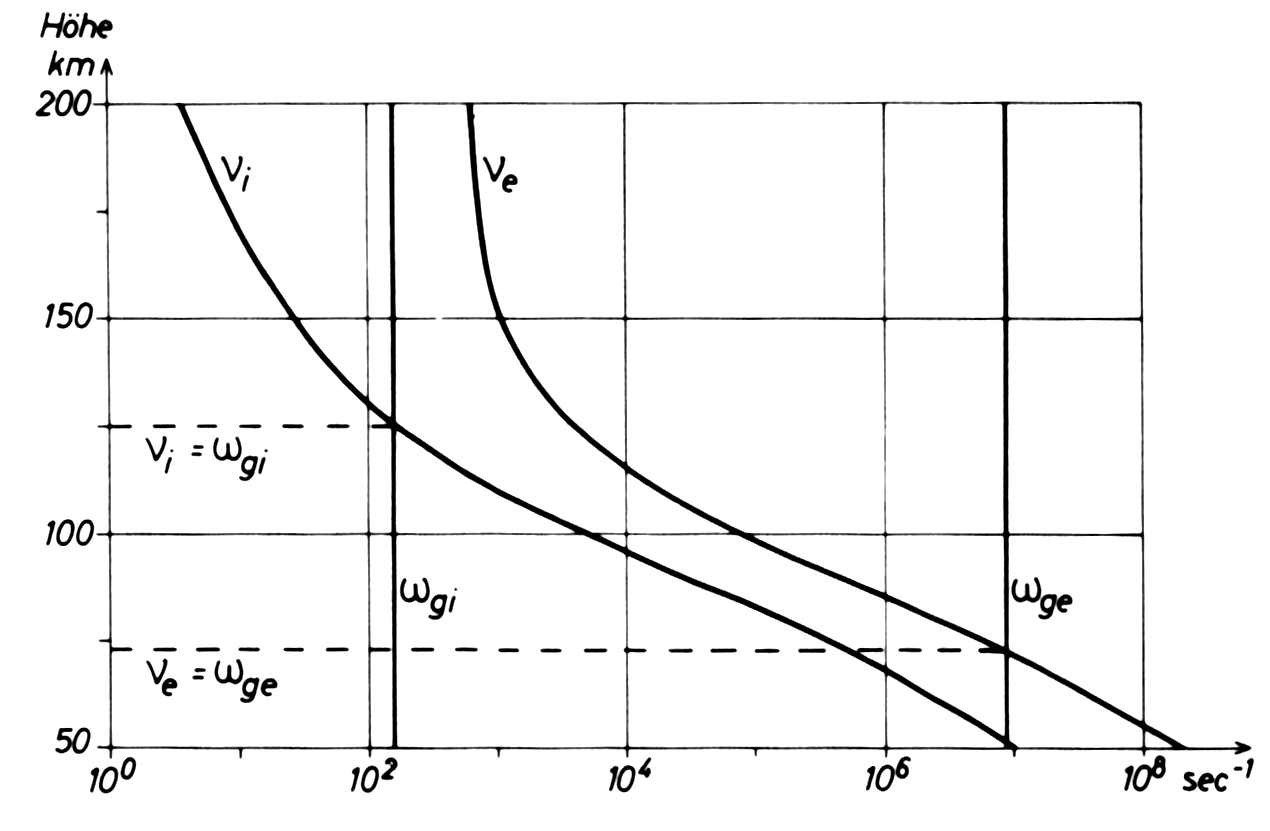
\includegraphics{./images/hoehenabh_stossfreq.png}

}

\caption{Höhenabhängigkeit der Stoßfrequenz für Ionen und Elektronen in
der unteren Ionosphäre in mittleren Breiten. Die gestrichelten Linien
begrenzen die Dynamoschicht (aus (Kertz 1971)).}

\end{figure}

\begin{figure}

{\centering 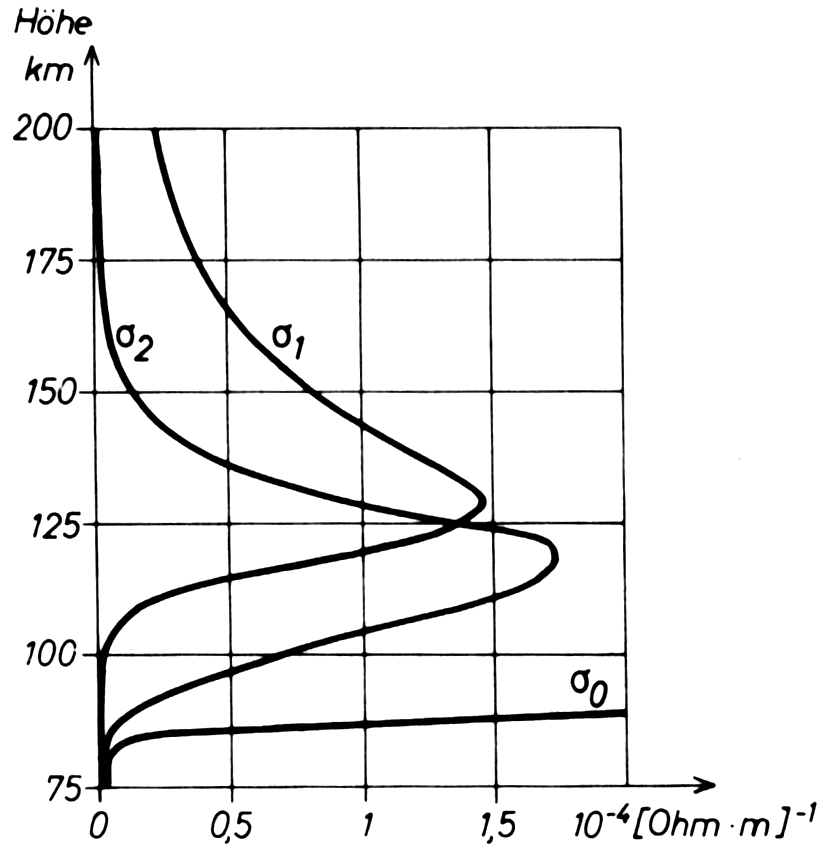
\includegraphics{./images/hoehenabh_leitf.png}

}

\caption{Höhenabhängigkeit der ionosphärischen Leitfähigkeiten (aus
(Kertz 1971))}

\end{figure}

\hypertarget{der-uxe4quatoriale-elektrojet-eej}{%
\section{Der äquatoriale Elektrojet
(EEJ)}\label{der-uxe4quatoriale-elektrojet-eej}}

\begin{figure}

{\centering 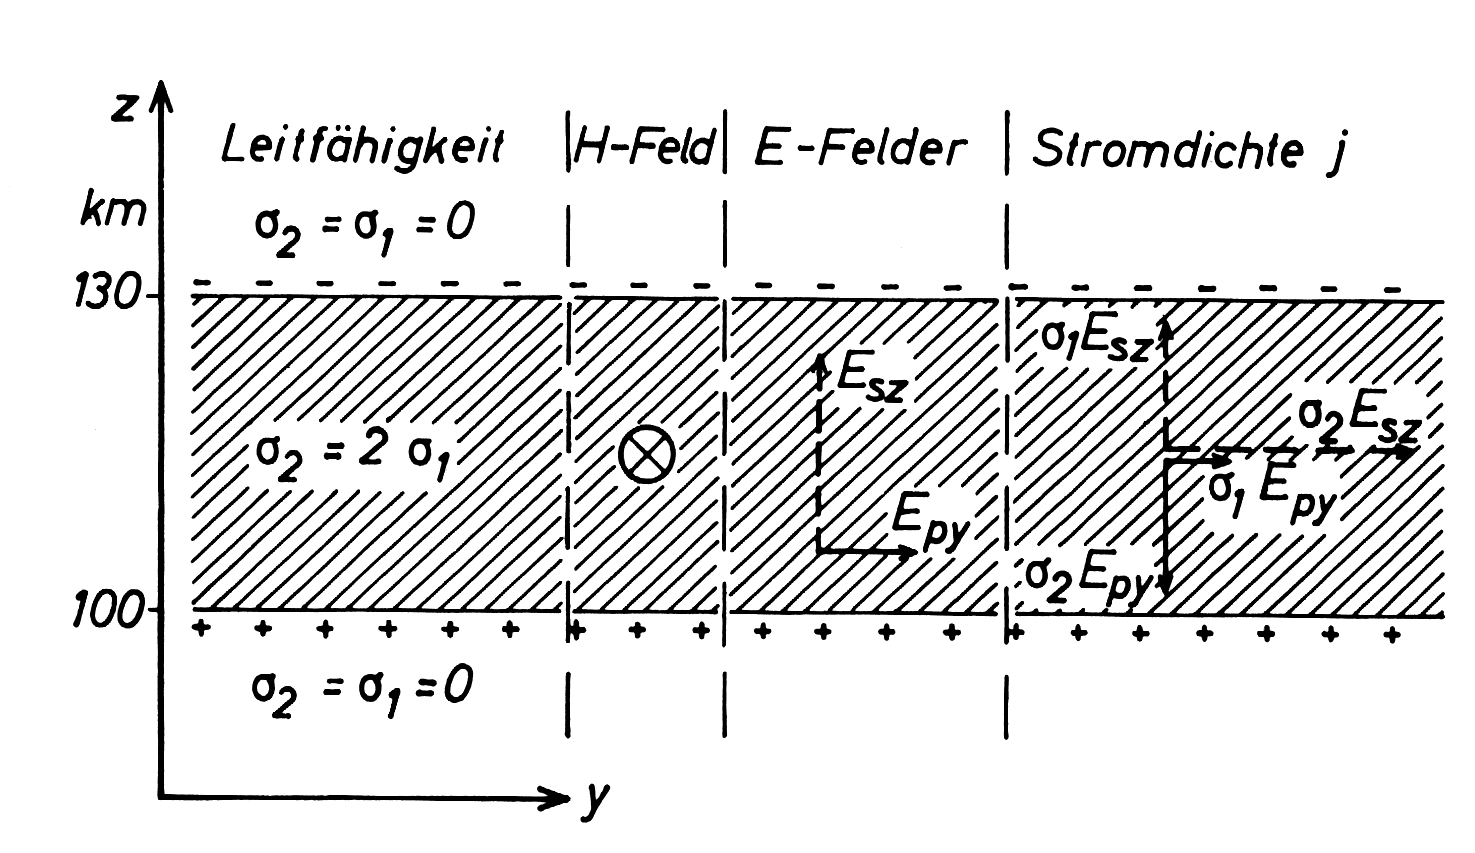
\includegraphics{./images/aequator_leitf.png}

}

\caption{Schematische Darstellung der Erhöhung der effektiven
Leitfähigkeit am magnetischen Äquator. y-Achse nach magnetisch Ost (aus
(Kertz 1971)).}

\end{figure}

\part{Das erdmagnetische Außenfeld}

\hypertarget{ionosphuxe4re}{%
\chapter{Ionosphäre}\label{ionosphuxe4re}}

\hypertarget{variationen}{%
\chapter{Variationen}\label{variationen}}

\bookmarksetup{startatroot}

\hypertarget{phuxe4nomene-im-system-der-magnetosphuxe4re-und-ionosphuxe4re}{%
\chapter{Phänomene im System der Magnetosphäre und
Ionosphäre}\label{phuxe4nomene-im-system-der-magnetosphuxe4re-und-ionosphuxe4re}}

\bookmarksetup{startatroot}

\hypertarget{zusammenfassung-1}{%
\chapter{Zusammenfassung}\label{zusammenfassung-1}}

\bookmarksetup{startatroot}

\hypertarget{literaturverzeichnis}{%
\chapter*{Literaturverzeichnis}\label{literaturverzeichnis}}
\addcontentsline{toc}{chapter}{Literaturverzeichnis}

\markboth{Literaturverzeichnis}{Literaturverzeichnis}

\hypertarget{refs}{}
\begin{CSLReferences}{1}{0}
\leavevmode\vadjust pre{\hypertarget{ref-debye1923debye}{}}%
Debye, P. \& Hückel, E. (1923) On the Debye length in strong
electrolytes. \emph{Physikalische Zeitschrift}, \textbf{24}, 185.

\leavevmode\vadjust pre{\hypertarget{ref-debye1923theorie}{}}%
Debye, P. \& Hückel, E. (1923) {Zur Theorie der Elektrolyte. II. Das
Grenzgesetz f{ü}r die elektrische Leitf{ä}higkeit}. \emph{Physikalische
Zeitschrift}, \textbf{24}, 305--325.

\leavevmode\vadjust pre{\hypertarget{ref-gibbon}{}}%
Gibbon, P. (2016) Introduction to Plasma Physics. \emph{CERN Yellow
Reports}, Vol 1 (2016): Proceedings of the 2014 CAS--CERN Accelerator
School: Plasma Wake Acceleration, CERN, Geneva.
doi:\href{https://doi.org/10.5170/CERN-2016-001.51}{10.5170/CERN-2016-001.51}

\leavevmode\vadjust pre{\hypertarget{ref-kertz}{}}%
Kertz, W. (1971) {Einf{ü}hrung in die Geophysik II}.
\emph{Bibliographisches Institut, Mannheim}.

\leavevmode\vadjust pre{\hypertarget{ref-thorne2017modern}{}}%
Thorne, K.S. \& Blandford, R.D. (2017) \emph{Modern classical physics:
optics, fluids, plasmas, elasticity, relativity, and statistical
physics}, Princeton University Press.

\end{CSLReferences}



\end{document}
